\documentclass[12pt,a4paper]{article}

% Essential packages
\usepackage[utf8]{inputenc}
\usepackage[T1]{fontenc}
\usepackage{amsmath,amssymb,amsfonts}
\usepackage{graphicx}
\usepackage{float}
\usepackage[margin=1in]{geometry}
\usepackage{hyperref}
\usepackage{fancyhdr}
\usepackage{tikz}
\usepackage{pgfplots}
\pgfplotsset{compat=1.17}
\usepackage{tcolorbox}
\usepackage{booktabs}
\usepackage{enumitem}
\usepackage{xcolor}

% Fix header height
\setlength{\headheight}{14.5pt}

% Color definitions
\definecolor{conceptblue}{RGB}{230,240,255}
\definecolor{exampleorange}{RGB}{255,245,230}
\definecolor{importantred}{RGB}{255,235,235}
\definecolor{deepgreen}{RGB}{220,245,220}
\definecolor{mathpurple}{RGB}{245,235,255}

% Custom environments
\newtcolorbox{conceptbox}[1][]{
    colback=conceptblue,
    colframe=blue!60!black,
    title=#1,
    fonttitle=\bfseries,
    boxrule=0.5pt,
    arc=3pt
}

\newtcolorbox{examplebox}[1][]{
    colback=exampleorange,
    colframe=orange!80!black,
    title=#1,
    fonttitle=\bfseries,
    boxrule=0.5pt,
    arc=3pt
}

\newtcolorbox{importantbox}{
    colback=importantred,
    colframe=red!70!black,
    boxrule=0.5pt,
    arc=3pt
}

\newtcolorbox{deepexplanation}{
    colback=deepgreen,
    colframe=green!50!black,
    boxrule=1pt,
    arc=4pt,
    left=8pt,
    right=8pt,
    top=8pt,
    bottom=8pt
}

\newtcolorbox{mathbox}{
    colback=mathpurple,
    colframe=purple!60!black,
    boxrule=0.5pt,
    arc=3pt
}

% Header/Footer
\pagestyle{fancy}
\fancyhf{}
\fancyhead[L]{Chapter 4: Filtering in the Frequency Domain}
\fancyhead[R]{Digital Image Processing}
\fancyfoot[C]{\thepage}

\title{\textbf{Chapter 4: Filtering in the Frequency Domain}\\
\Large Comprehensive Study Notes with Deep Technical Analysis\\
\normalsize Based on Gonzalez \& Woods (3rd Edition) and CPE415 Lectures}
\author{Study Notes - Version 3 (Deep Technical Explanations)}
\date{Spring 2026}

\begin{document}

\maketitle
\tableofcontents
\newpage

%==============================================================================
\section{Introduction: Why Frequency Domain?}
%==============================================================================

Before diving into the mathematics, let's understand \textbf{why} we transform images to the frequency domain.

\begin{conceptbox}[The Core Insight]
Every image can be decomposed into a sum of sinusoidal waves of different frequencies, orientations, and amplitudes. Some operations that are \textbf{computationally expensive} in the spatial domain become \textbf{simple multiplications} in the frequency domain.
\end{conceptbox}

\subsection{Spatial Domain vs. Frequency Domain}

In the \textbf{spatial domain}, we work directly with pixel values $f(x, y)$. Operations involve convolution:
\[
g(x, y) = f(x, y) * h(x, y) = \sum_{s=-a}^{a} \sum_{t=-b}^{b} f(s, t) \cdot h(x-s, y-t)
\]

In the \textbf{frequency domain}, convolution becomes multiplication:
\[
G(u, v) = F(u, v) \cdot H(u, v)
\]

\begin{figure}[H]
    \centering
    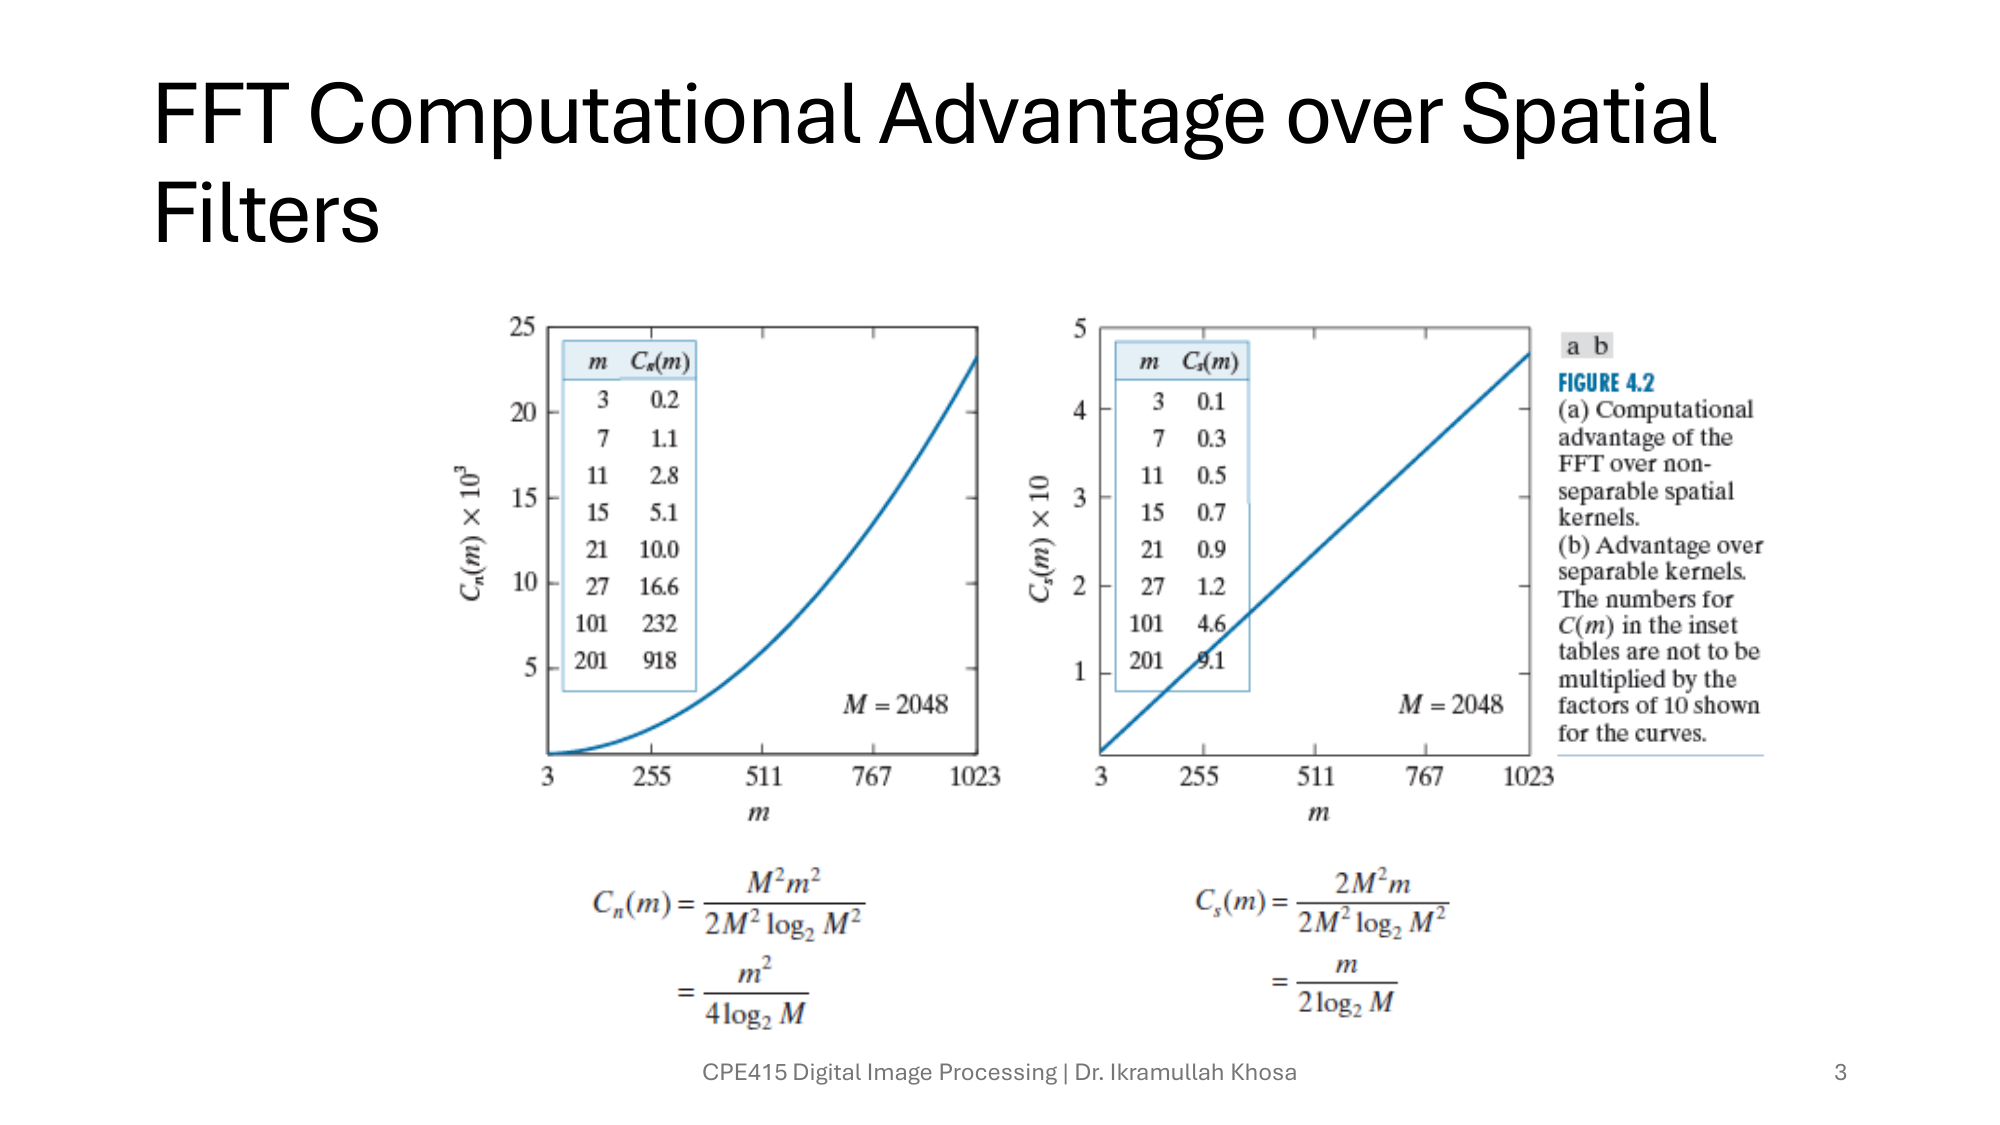
\includegraphics[width=0.85\textwidth]{images/slide8-03.png}
    \caption{FFT computational advantage over spatial filtering}
    \label{fig:fft_advantage}
\end{figure}

\begin{deepexplanation}
\textbf{DEEP ANALYSIS - Figure \ref{fig:fft_advantage}: Why FFT is Computationally Superior}

\textbf{The Computational Cost Problem:}
Consider convolving an $N \times N$ image with an $M \times M$ filter kernel in the spatial domain:
\begin{itemize}
    \item For \textbf{each} output pixel, we must perform $M^2$ multiplications and $M^2 - 1$ additions
    \item Total output pixels: $N^2$
    \item \textbf{Total operations: $O(N^2 \cdot M^2)$}
    \item For a 1024×1024 image with a 64×64 kernel: $\approx 4.3 \times 10^9$ operations
\end{itemize}

\textbf{The FFT Revolution:}
The Fast Fourier Transform (Cooley-Tukey, 1965) reduces the DFT from $O(N^2)$ to $O(N \log N)$:
\begin{itemize}
    \item FFT of image: $O(N^2 \log N)$ operations
    \item FFT of filter: $O(N^2 \log N)$ operations
    \item Pointwise multiplication: $O(N^2)$ operations
    \item Inverse FFT: $O(N^2 \log N)$ operations
    \item \textbf{Total: $O(N^2 \log N)$}
\end{itemize}

\textbf{Crossover Point:}
The frequency domain approach becomes faster when:
\[
N^2 M^2 > c \cdot N^2 \log N \implies M > \sqrt{c \cdot \log N}
\]
For typical implementations, this crossover occurs around $M \approx 32$ for a 512×512 image.

\textbf{Physical Interpretation:}
The convolution theorem ($f * h \leftrightarrow F \cdot H$) means that sliding a filter across every pixel (spatial convolution) is mathematically equivalent to scaling each frequency component by the filter's response at that frequency. The latter requires far fewer operations because frequencies are ``global'' properties.
\end{deepexplanation}

%==============================================================================
\section{Mathematical Foundations: Fourier Series}
%==============================================================================

\subsection{The Fundamental Theorem of Fourier Analysis}

Jean-Baptiste Fourier (1807) proved that \textbf{any periodic function} can be represented as a sum of sines and cosines.

\begin{mathbox}
\textbf{Fourier Series Representation:}
For a periodic function $f(t)$ with period $T$:
\[
f(t) = a_0 + \sum_{n=1}^{\infty} \left[ a_n \cos\left(\frac{2\pi n t}{T}\right) + b_n \sin\left(\frac{2\pi n t}{T}\right) \right]
\]
where the coefficients are:
\[
a_0 = \frac{1}{T} \int_{0}^{T} f(t) \, dt \quad \text{(DC component / average)}
\]
\[
a_n = \frac{2}{T} \int_{0}^{T} f(t) \cos\left(\frac{2\pi n t}{T}\right) dt, \quad
b_n = \frac{2}{T} \int_{0}^{T} f(t) \sin\left(\frac{2\pi n t}{T}\right) dt
\]
\end{mathbox}

\subsection{The Impulse Function (Dirac Delta)}

The impulse function is a mathematical idealization --- infinitely tall, infinitely narrow, but with unit area.

\begin{figure}[H]
    \centering
    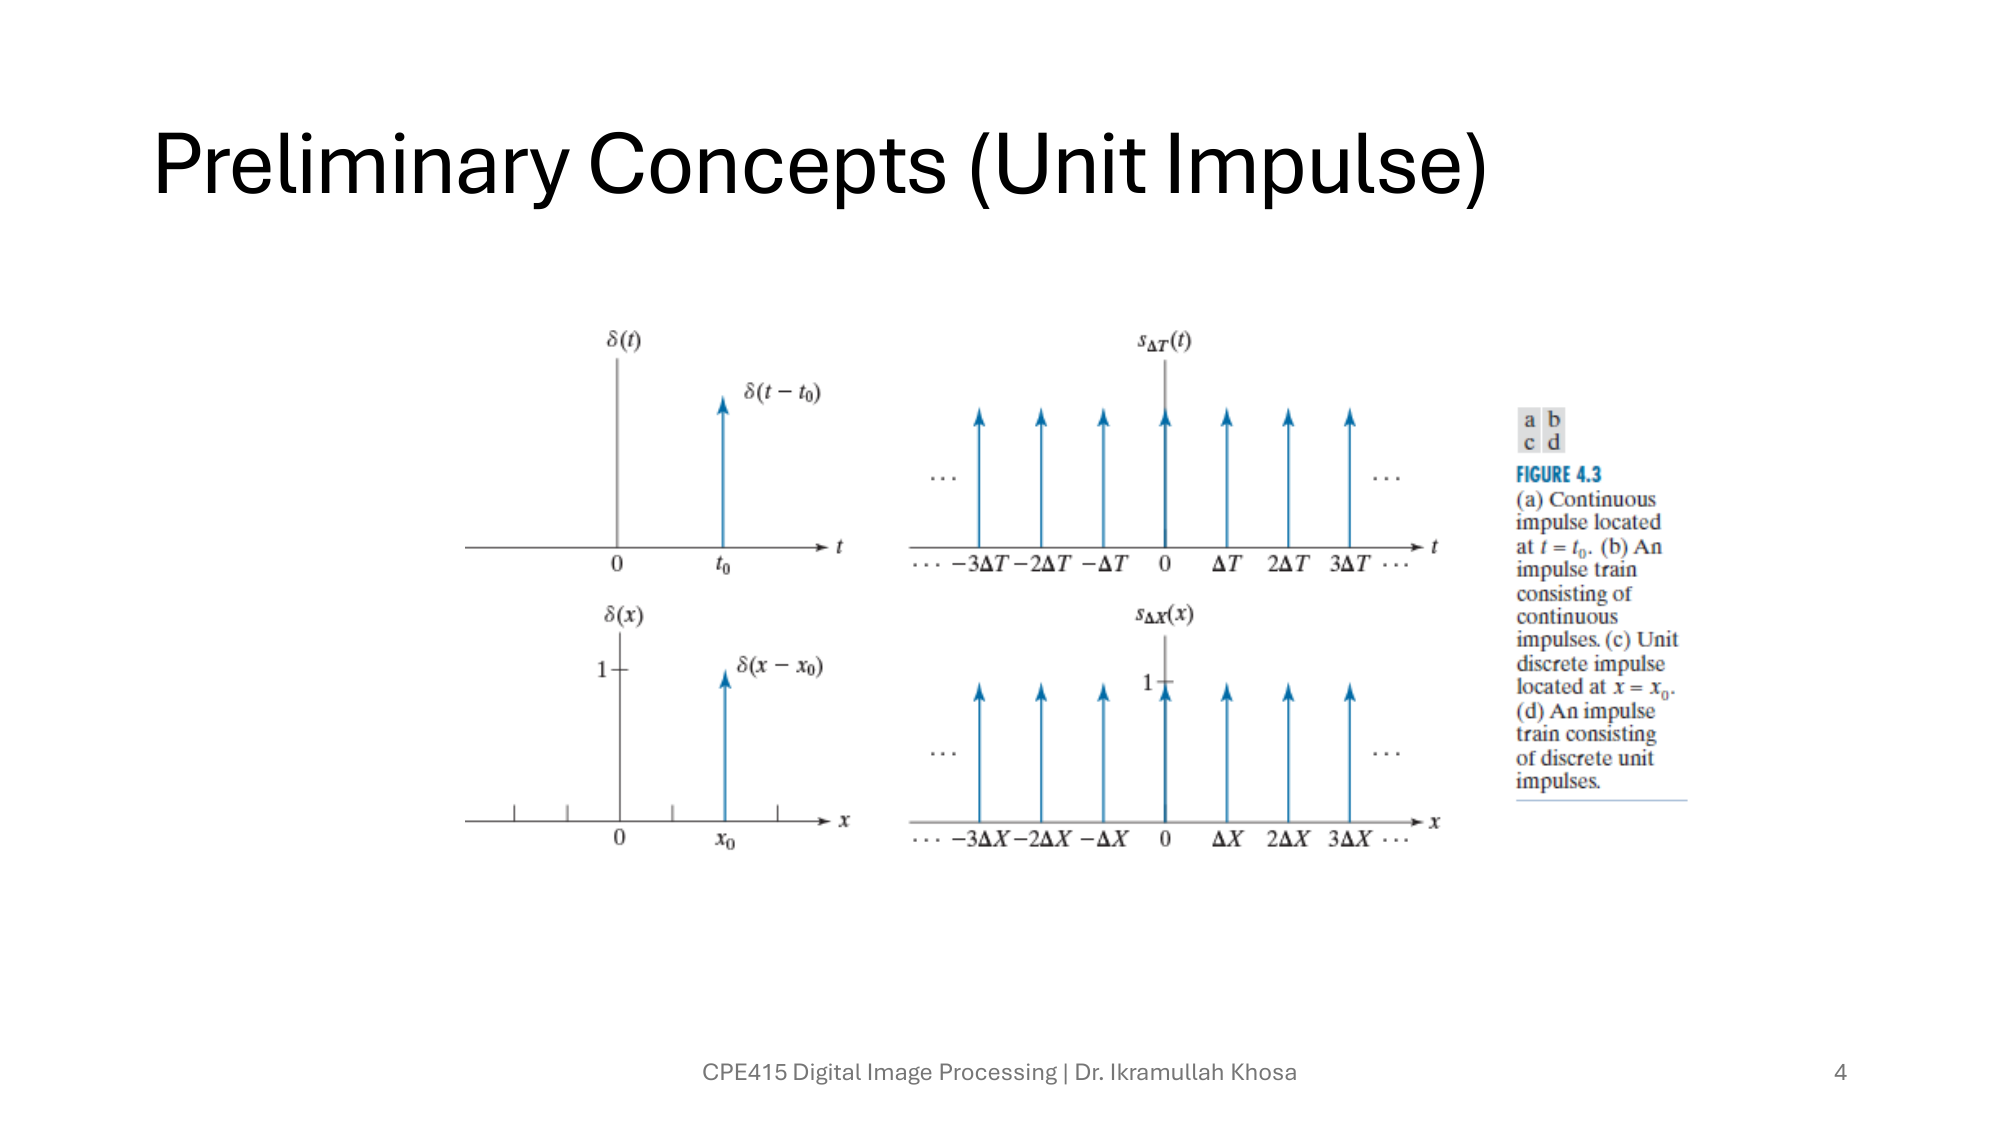
\includegraphics[width=0.7\textwidth]{images/slide8-04.png}
    \caption{Unit impulse function and impulse trains (FIGURE 4.3)}
    \label{fig:impulse}
\end{figure}

\begin{deepexplanation}
\textbf{DEEP ANALYSIS - Figure \ref{fig:impulse}: The Dirac Delta Function}

\textbf{Mathematical Definition:}
The Dirac delta function $\delta(t)$ is defined by two properties:
\[
\delta(t) = \begin{cases} \infty & t = 0 \\ 0 & t \neq 0 \end{cases}
\quad \text{with} \quad \int_{-\infty}^{\infty} \delta(t) \, dt = 1
\]

\textbf{The Sifting Property (Why It Matters for Sampling):}
\[
\int_{-\infty}^{\infty} f(t) \delta(t - t_0) \, dt = f(t_0)
\]
This ``sifts out'' the value of $f$ at exactly $t = t_0$. This is precisely what happens during sampling --- we extract the function's value at discrete points.

\textbf{Physical Interpretation:}
Imagine hitting a drum with an infinitely brief, infinitely strong tap that delivers exactly 1 unit of energy. The drum's response to this impulse reveals its complete frequency response. Similarly, the impulse function contains \textbf{all frequencies equally}:
\[
\mathcal{F}\{\delta(t)\} = 1 \quad \text{(constant for all frequencies)}
\]

\textbf{Why This Shape in the Figure:}
The figure shows a practical approximation --- a very narrow, tall rectangle or triangle approaching the ideal. In reality, no physical system can produce a true impulse, but short pulses approximate it well for band-limited systems.

\textbf{Connection to Sampling:}
When we sample a continuous signal, we multiply it by an impulse train (series of deltas). Each impulse ``picks out'' one sample value. This multiplication in time domain becomes convolution in frequency domain, which is the origin of spectral replication (and potential aliasing).
\end{deepexplanation}

\subsection{The Box (Rectangular) Function}

\begin{figure}[H]
    \centering
    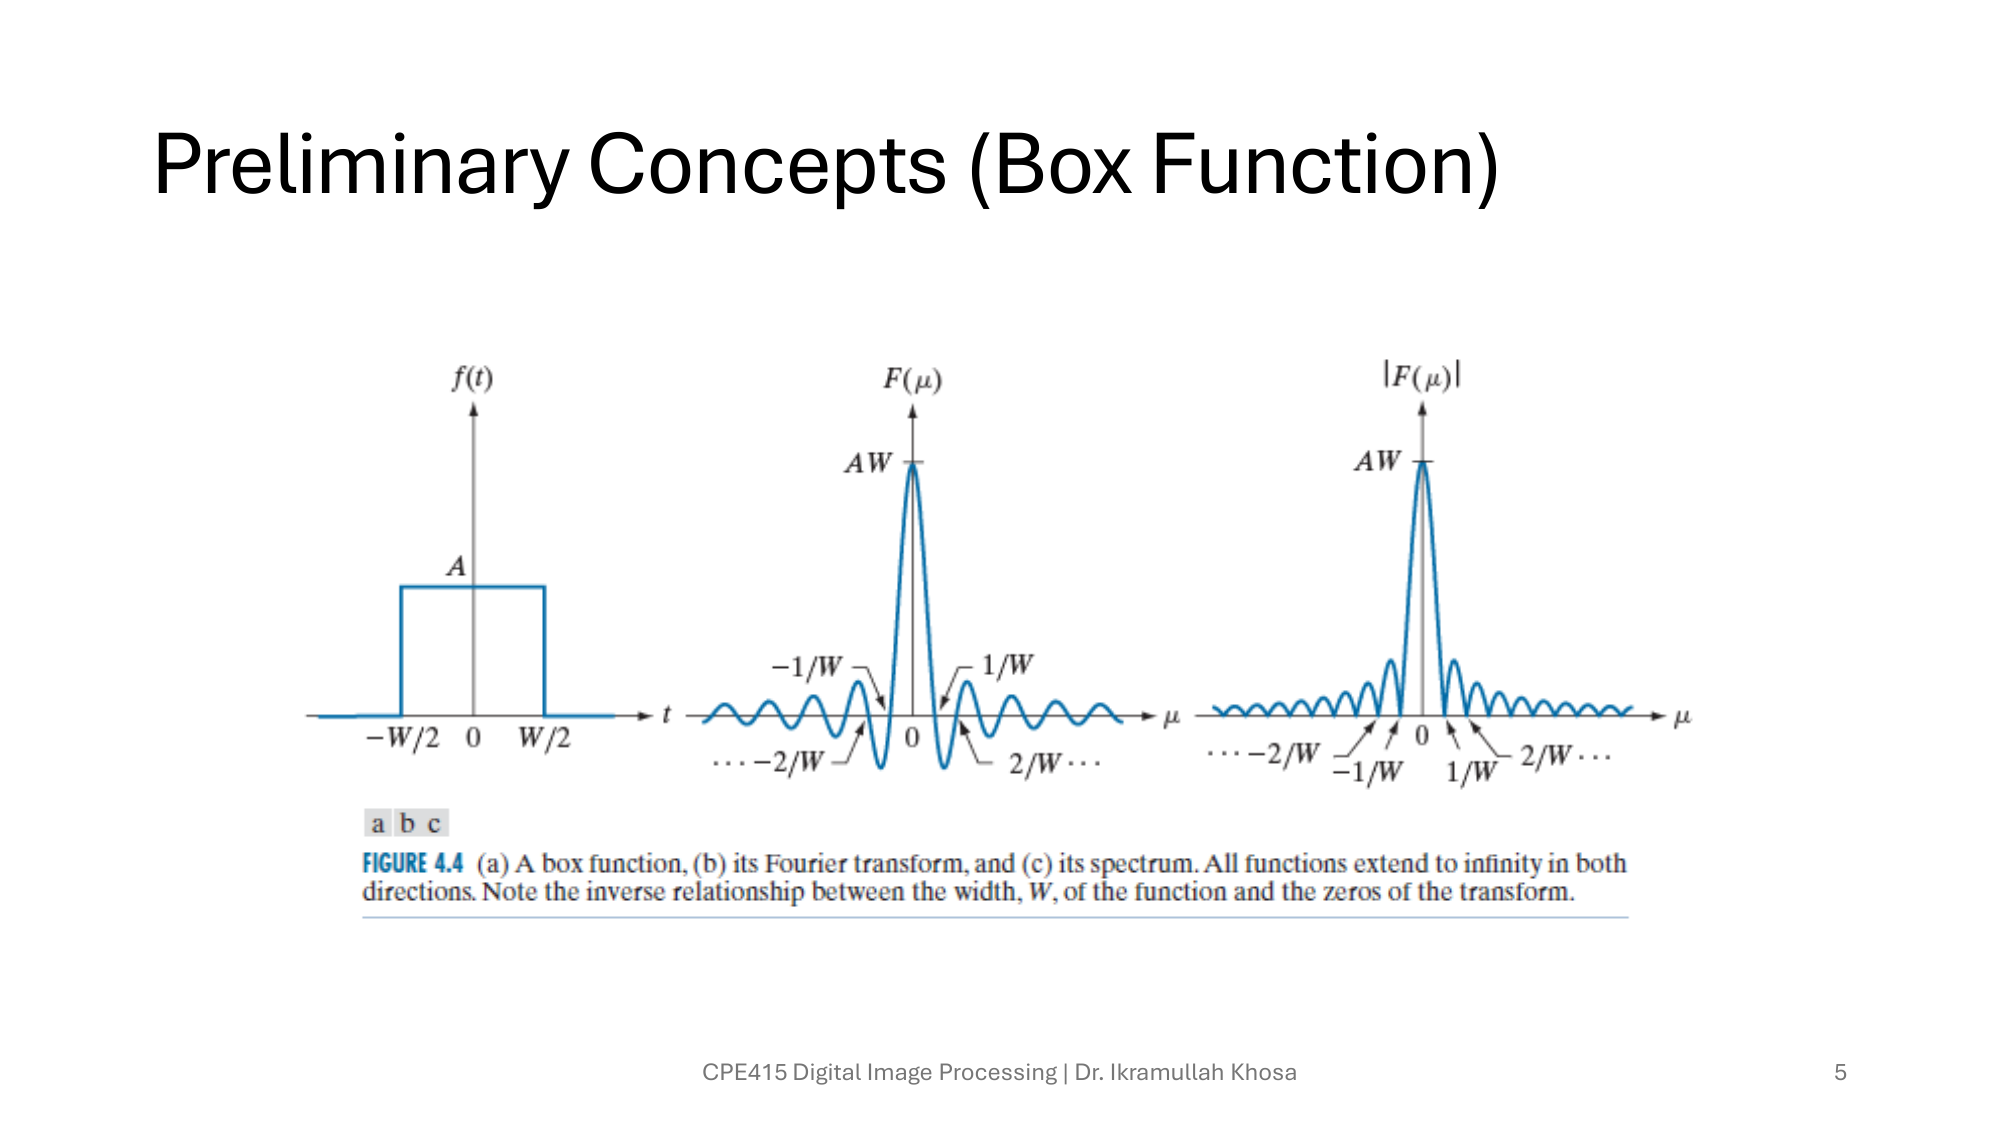
\includegraphics[width=0.7\textwidth]{images/slide8-05.png}
    \caption{Box function and its Fourier transform (sinc) (FIGURE 4.4)}
    \label{fig:box}
\end{figure}

\begin{deepexplanation}
\textbf{DEEP ANALYSIS - Figure \ref{fig:box}: The Box Function and Its Transform}

\textbf{Definition:}
\[
\text{rect}(t/W) = \begin{cases} 1 & |t| \leq W/2 \\ 0 & |t| > W/2 \end{cases}
\]

\textbf{Fourier Transform --- The Sinc Function:}
\[
\mathcal{F}\{\text{rect}(t/W)\} = W \cdot \text{sinc}(Wf) = W \cdot \frac{\sin(\pi W f)}{\pi W f}
\]

\textbf{Why the Sinc Shape Emerges (Physical Intuition):}
\begin{enumerate}
    \item A sharp rectangular cutoff in one domain creates \textbf{infinite ripples} in the other domain
    \item The abrupt edges of the box contain high-frequency components (sharp transitions require high frequencies)
    \item The sinc function oscillates forever, decaying as $1/f$ --- representing these ``edge frequencies''
\end{enumerate}

\textbf{Critical Insight --- The Uncertainty Principle:}
\[
\Delta t \cdot \Delta f \geq \frac{1}{4\pi}
\]
A narrow box (small $W$) produces a wide sinc (spread across many frequencies). A wide box produces a narrow sinc. You cannot have a signal localized in both time AND frequency simultaneously.

\textbf{Connection to Image Processing:}
\begin{itemize}
    \item \textbf{Ideal lowpass filter} = box in frequency domain = sinc in spatial domain
    \item Applying an ideal lowpass filter means convolving with a sinc, which extends infinitely (ringing artifacts)
    \item The ``ringing'' near sharp edges in filtered images is the spatial manifestation of this Fourier pair
\end{itemize}
\end{deepexplanation}

%==============================================================================
\section{The Continuous Fourier Transform}
%==============================================================================

\subsection{Definition and Properties}

\begin{mathbox}
\textbf{Forward Fourier Transform:}
\[
F(u) = \int_{-\infty}^{\infty} f(t) e^{-j2\pi ut} \, dt
\]
\textbf{Inverse Fourier Transform:}
\[
f(t) = \int_{-\infty}^{\infty} F(u) e^{j2\pi ut} \, du
\]
\end{mathbox}

The complex exponential can be expanded using Euler's formula:
\[
e^{j\theta} = \cos(\theta) + j\sin(\theta)
\]

\subsection{Key Fourier Transform Pairs}

Understanding these fundamental pairs is essential:

\begin{center}
\begin{tabular}{|c|c|l|}
\hline
\textbf{Time/Space Domain} & \textbf{Frequency Domain} & \textbf{Significance} \\
\hline
$\delta(t)$ & $1$ & Impulse has all frequencies \\
$1$ & $\delta(f)$ & Constant has only DC \\
$\cos(2\pi f_0 t)$ & $\frac{1}{2}[\delta(f-f_0) + \delta(f+f_0)]$ & Single frequency \\
$\text{rect}(t)$ & $\text{sinc}(f)$ & Sharp edges $\leftrightarrow$ ripples \\
$\text{sinc}(t)$ & $\text{rect}(f)$ & Ideal filter \\
Gaussian & Gaussian & Self-similar (optimal localization) \\
\hline
\end{tabular}
\end{center}

%==============================================================================
\section{Sampling Theory: The Heart of Digital Processing}
%==============================================================================

Sampling converts a continuous signal $f(t)$ into a discrete sequence $f[n] = f(n \cdot \Delta T)$.

\subsection{The Sampling Process}

\begin{figure}[H]
    \centering
    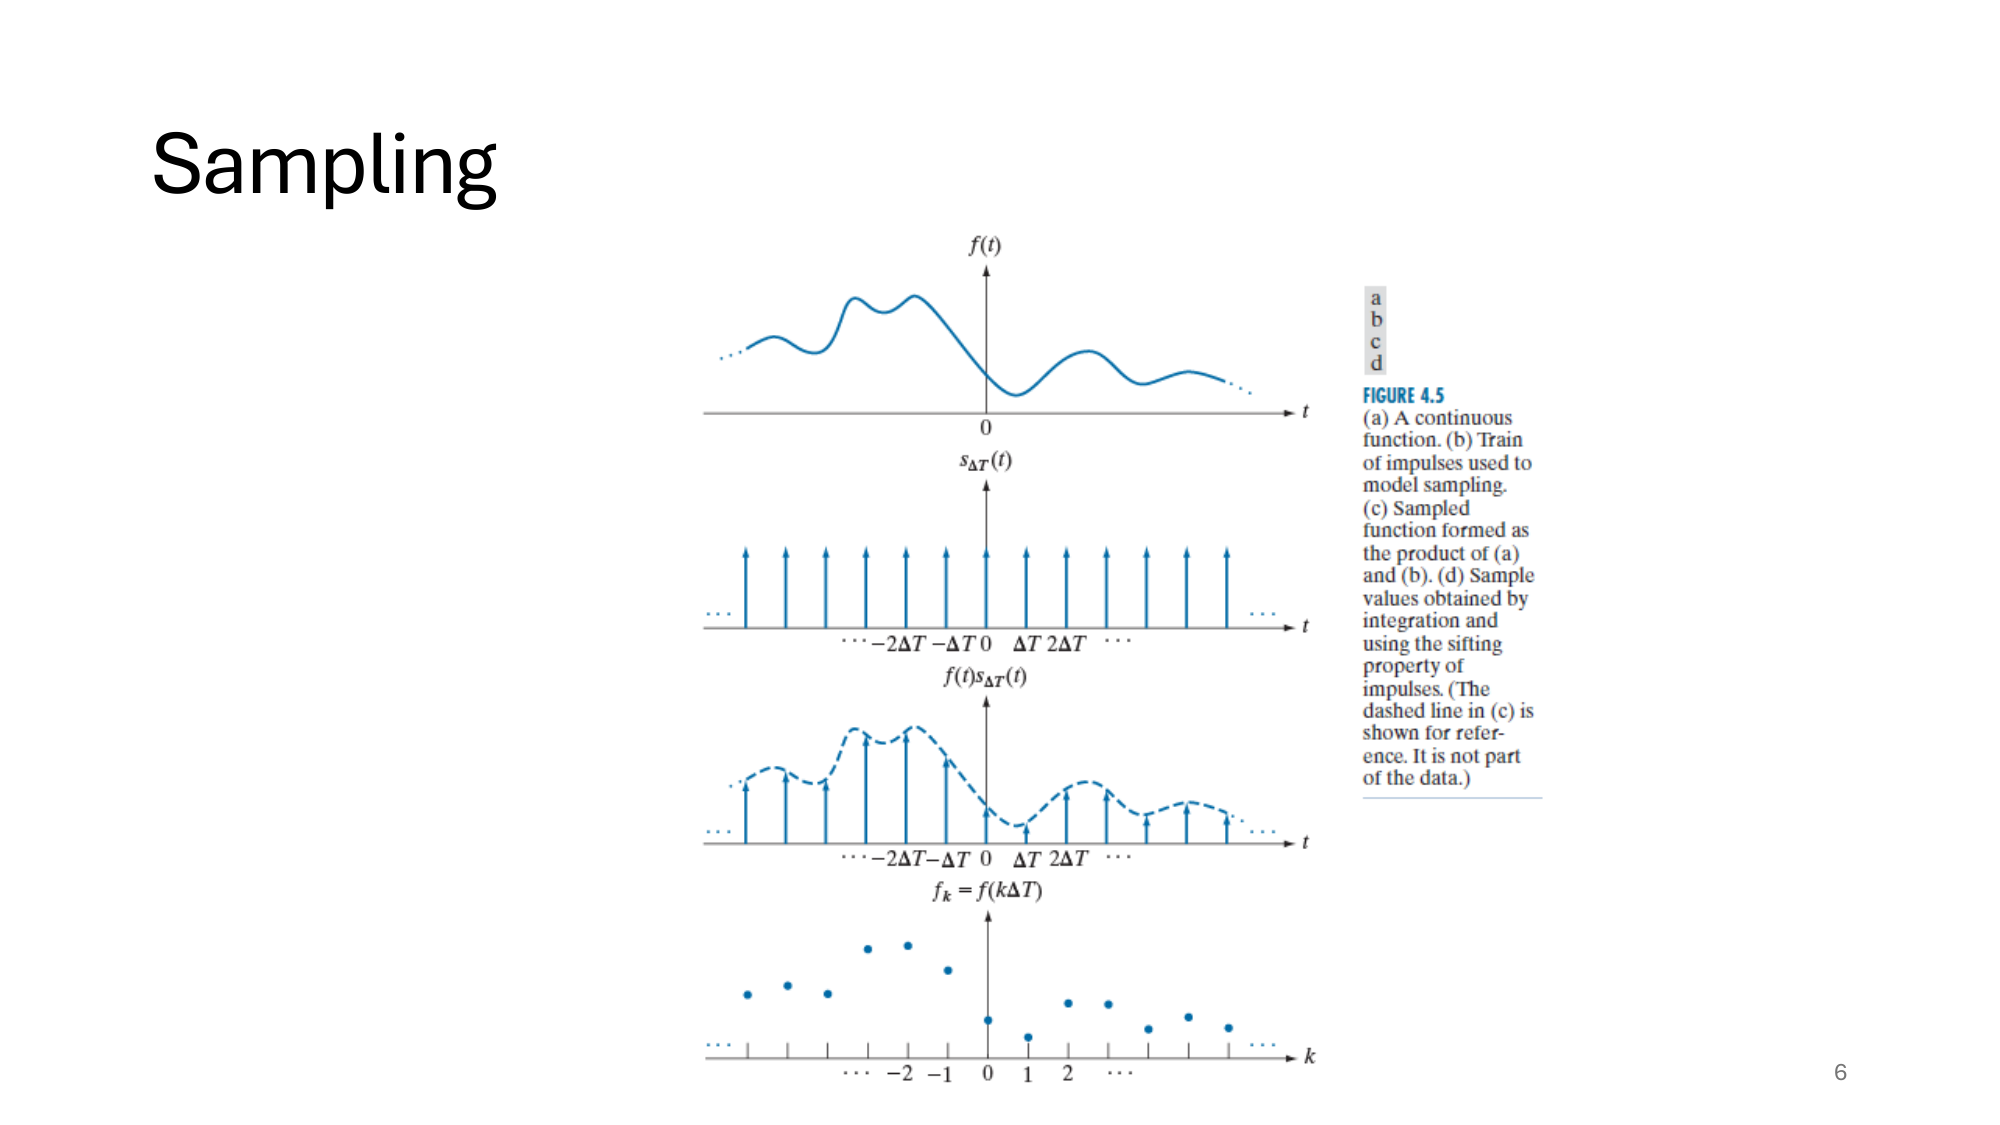
\includegraphics[width=0.85\textwidth]{images/slide8-06.png}
    \caption{Sampling a continuous function using an impulse train (FIGURE 4.5)}
    \label{fig:sampling}
\end{figure}

\begin{deepexplanation}
\textbf{DEEP ANALYSIS - Figure \ref{fig:sampling}: How Sampling Works Mathematically}

\textbf{The Sampling Operation:}
Mathematically, sampling multiplies the continuous signal by an impulse train:
\[
\tilde{f}(t) = f(t) \cdot s_{\Delta T}(t) = f(t) \cdot \sum_{n=-\infty}^{\infty} \delta(t - n\Delta T)
\]
where $\Delta T$ is the sampling interval and $1/\Delta T$ is the sampling frequency.

\textbf{Step-by-Step What Happens:}
\begin{enumerate}
    \item \textbf{Original signal $f(t)$}: Continuous, contains frequencies from 0 to some maximum $f_{max}$
    \item \textbf{Impulse train $s_{\Delta T}(t)$}: Infinite series of delta functions spaced $\Delta T$ apart
    \item \textbf{Multiplication}: Each impulse ``grabs'' the signal value at that instant
    \item \textbf{Result}: A weighted impulse train where each impulse's height equals $f(n\Delta T)$
\end{enumerate}

\textbf{What the Figure Shows:}
\begin{itemize}
    \item Top: The original continuous signal (smooth curve)
    \item Middle: The impulse train (vertical arrows at regular intervals)
    \item Bottom: The sampled signal (impulses with heights matching the original signal)
\end{itemize}

\textbf{Frequency Domain Consequence:}
Multiplication in time $\rightarrow$ convolution in frequency:
\[
\tilde{F}(u) = F(u) * S(u)
\]
Since the Fourier transform of an impulse train is another impulse train (with spacing $1/\Delta T$), the convolution creates infinite copies of the original spectrum, spaced $1/\Delta T$ apart. This is the origin of both perfect reconstruction (if copies don't overlap) and aliasing (if they do).
\end{deepexplanation}

\subsection{Spectrum of a Sampled Signal}

\begin{figure}[H]
    \centering
    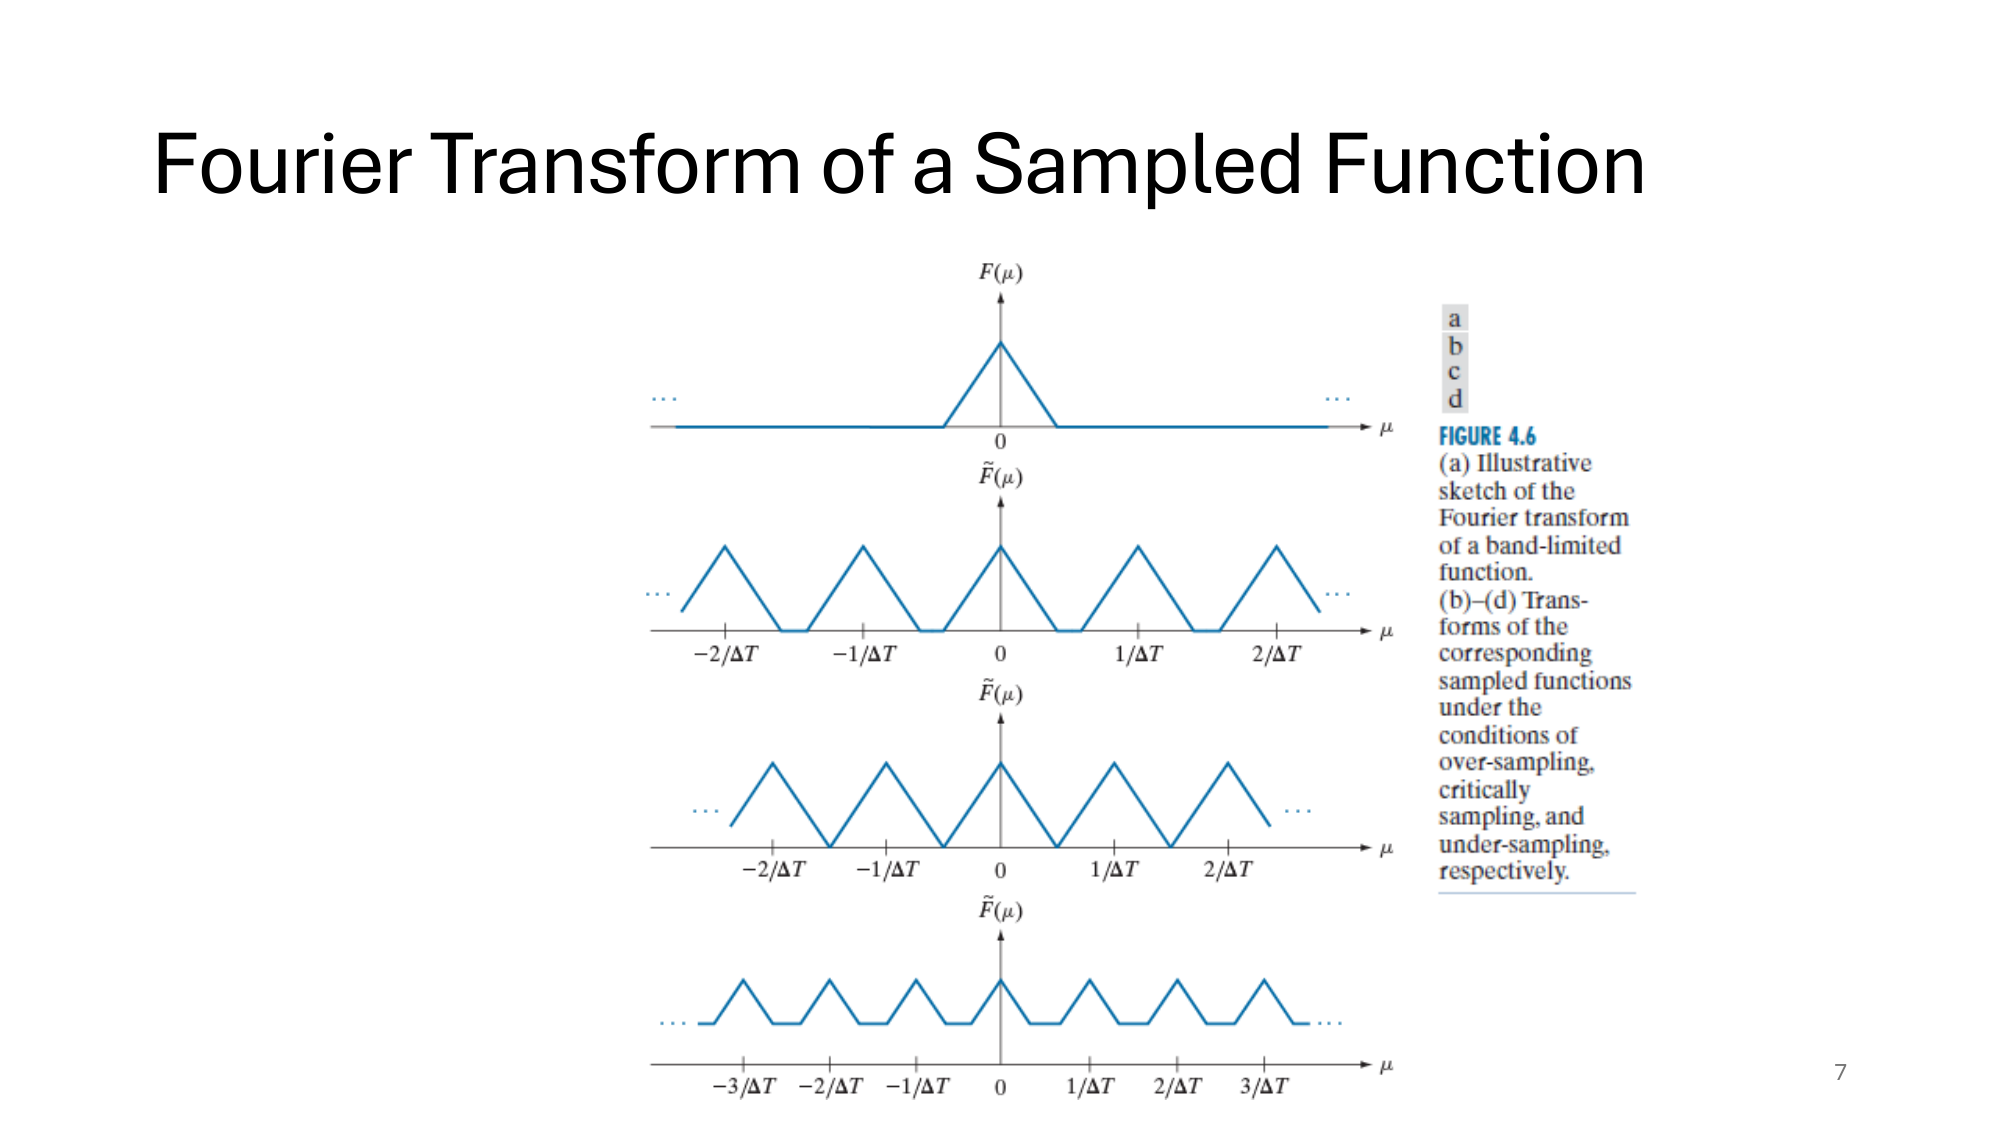
\includegraphics[width=0.85\textwidth]{images/slide8-07.png}
    \caption{Fourier transform of sampled functions: oversampling, critical sampling, and undersampling (FIGURE 4.6)}
    \label{fig:sampled_spectrum}
\end{figure}

\begin{deepexplanation}
\textbf{DEEP ANALYSIS - Figure \ref{fig:sampled_spectrum}: Why Sampling Creates Spectrum Copies}

\textbf{The Mathematical Mechanism:}
The Fourier transform of an impulse train with period $\Delta T$ is:
\[
\mathcal{F}\left\{ \sum_{n=-\infty}^{\infty} \delta(t - n\Delta T) \right\} = \frac{1}{\Delta T} \sum_{k=-\infty}^{\infty} \delta\left(f - \frac{k}{\Delta T}\right)
\]
This is another impulse train, but in frequency, with spacing $f_s = 1/\Delta T$.

\textbf{Convolution with Impulse Train:}
When we convolve $F(u)$ with this frequency-domain impulse train:
\[
\tilde{F}(u) = \frac{1}{\Delta T} \sum_{k=-\infty}^{\infty} F\left(u - \frac{k}{\Delta T}\right)
\]

Each impulse creates a complete copy of the original spectrum, shifted to that frequency location.

\textbf{What the Figure Illustrates:}
\begin{itemize}
    \item \textbf{Original spectrum} $F(u)$: Band-limited, extends from $-f_{max}$ to $+f_{max}$
    \item \textbf{Sampled spectrum} $\tilde{F}(u)$: Infinite copies centered at $0, \pm f_s, \pm 2f_s, ...$
    \item Each copy is identical to the original, just shifted
\end{itemize}

\textbf{Physical Interpretation:}
Sampling ``folds'' the frequency axis. High frequencies that exceed $f_s/2$ get ``reflected'' back into the $[-f_s/2, f_s/2]$ range, mixing with lower frequencies. This is aliasing.

\textbf{Why Copies Appear:}
The impulse train contains all harmonics of the sampling frequency. When you multiply by cosine terms (hidden in the complex exponential), you get sum and difference frequencies --- this is the same principle as AM radio modulation.
\end{deepexplanation}

\begin{figure}[H]
    \centering
    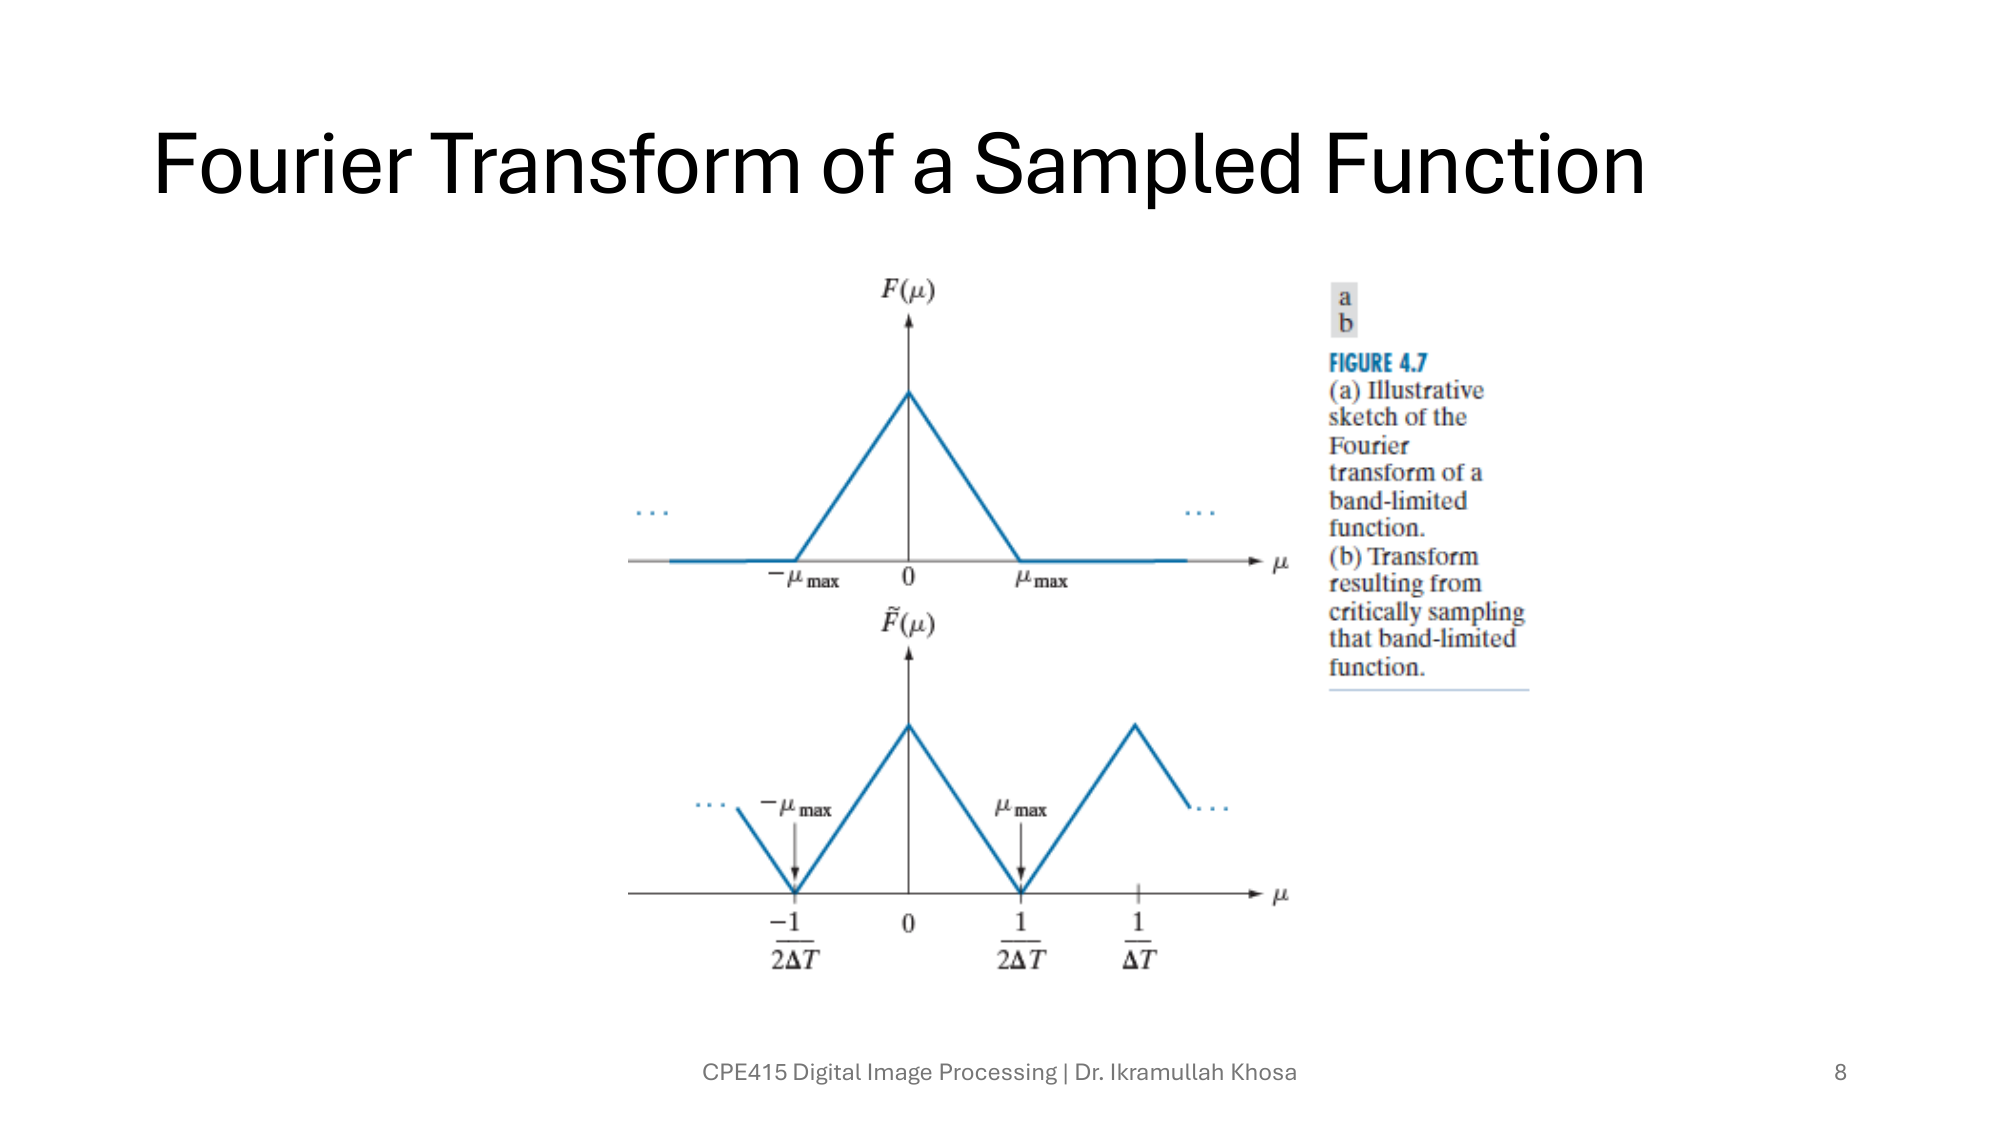
\includegraphics[width=0.85\textwidth]{images/slide8-08.png}
    \caption{Critical sampling of a band-limited function (FIGURE 4.7)}
    \label{fig:sampling_rate}
\end{figure}

\begin{deepexplanation}
\textbf{DEEP ANALYSIS - Figure \ref{fig:sampling_rate}: Sampling Rate vs. Spectrum Spacing}

\textbf{The Critical Relationship:}
The spacing between spectrum copies equals the sampling frequency $f_s = 1/\Delta T$.

\begin{itemize}
    \item \textbf{Higher sampling rate} ($\Delta T$ smaller) $\rightarrow$ copies further apart $\rightarrow$ less overlap risk
    \item \textbf{Lower sampling rate} ($\Delta T$ larger) $\rightarrow$ copies closer together $\rightarrow$ more overlap risk
\end{itemize}

\textbf{What the Figure Demonstrates:}
The figure likely shows multiple scenarios:
\begin{enumerate}
    \item \textbf{High sampling rate}: Large gaps between spectrum copies. The baseband copy (centered at 0) is well-separated from its neighbors.
    
    \item \textbf{Moderate sampling rate}: Spectrum copies are closer but still don't overlap. This is the ``just enough'' case.
    
    \item \textbf{Low sampling rate}: Copies overlap, causing aliasing.
\end{enumerate}

\textbf{The Critical Threshold:}
For no overlap, the distance between copy centers ($f_s$) must exceed twice the signal bandwidth ($2f_{max}$):
\[
f_s > 2f_{max} \quad \Leftrightarrow \quad \text{copies separated by more than signal width}
\]

\textbf{Practical Implication:}
In image sensors:
\begin{itemize}
    \item Pixel pitch determines $\Delta T$ (spatial sampling interval)
    \item Lens MTF (modulation transfer function) determines $f_{max}$
    \item Optical lowpass filter (OLPF) can reduce $f_{max}$ to prevent aliasing
\end{itemize}
\end{deepexplanation}

%==============================================================================
\section{The Nyquist-Shannon Sampling Theorem}
%==============================================================================

\begin{importantbox}
\textbf{Nyquist-Shannon Sampling Theorem:}
A band-limited signal with maximum frequency $f_{max}$ can be \textbf{perfectly reconstructed} from its samples if the sampling rate satisfies:
\[
f_s > 2 f_{max}
\]
The frequency $f_N = f_s/2$ is called the \textbf{Nyquist frequency} --- it's the highest frequency that can be represented without aliasing.
\end{importantbox}

\subsection{Proper Sampling (No Aliasing)}

\begin{figure}[H]
    \centering
    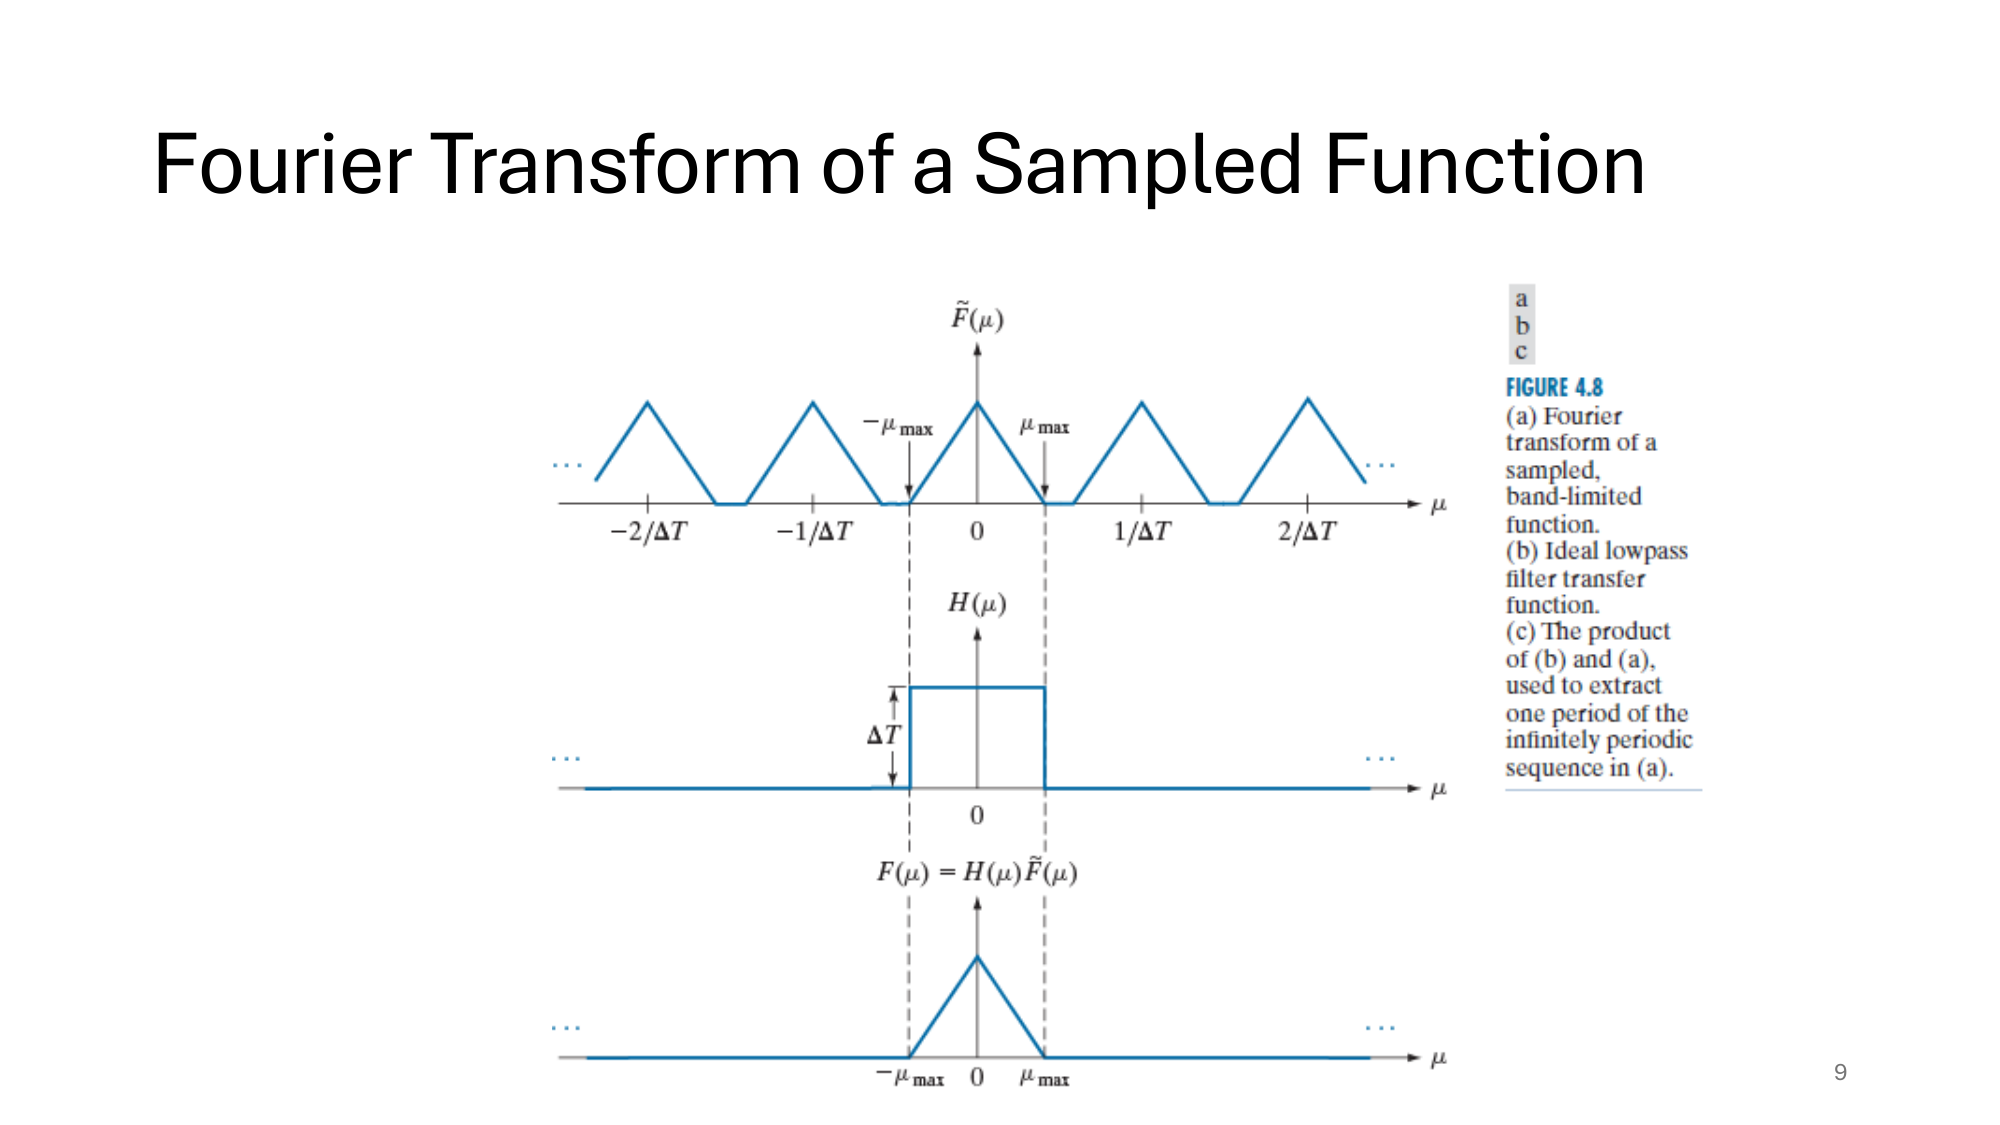
\includegraphics[width=0.85\textwidth]{images/slide8-09.png}
    \caption{Reconstruction using ideal lowpass filter to extract baseband (FIGURE 4.8)}
    \label{fig:proper_sampling}
\end{figure}

\begin{deepexplanation}
\textbf{DEEP ANALYSIS - Figure \ref{fig:proper_sampling}: Successful Sampling Without Information Loss}

\textbf{The Ideal Scenario:}
When $f_s > 2f_{max}$:
\begin{itemize}
    \item The baseband spectrum ($-f_{max}$ to $+f_{max}$) sits entirely within $[-f_s/2, +f_s/2]$
    \item The first copies are centered at $\pm f_s$, starting at $\pm(f_s - f_{max})$
    \item Since $f_s > 2f_{max}$, we have $f_s - f_{max} > f_{max}$, meaning no overlap
\end{itemize}

\textbf{What the Figure Shows:}
\begin{enumerate}
    \item The original spectrum (triangular or band-limited shape)
    \item Clear gaps between the baseband and the first spectral copies
    \item An ideal lowpass filter (shown as a rectangle) can isolate the baseband
\end{enumerate}

\textbf{Perfect Reconstruction Process:}
\begin{enumerate}
    \item Multiply sampled spectrum by ideal lowpass filter $H(f) = \text{rect}(f/f_s)$
    \item This removes all copies except the baseband
    \item Inverse Fourier transform recovers original continuous signal \textbf{exactly}
\end{enumerate}

\textbf{Mathematical Proof of Perfect Recovery:}
\[
F_{recovered}(u) = \tilde{F}(u) \cdot H(u) = F(u) \quad \text{for } |u| < f_s/2
\]

\textbf{Physical Analogy:}
Think of photocopying a document and placing copies side by side with gaps. You can easily cut out the original from the row. But if copies overlap, the overlapping text becomes unreadable --- that's aliasing.
\end{deepexplanation}

\subsection{Aliasing: When Sampling Fails}

\begin{figure}[H]
    \centering
    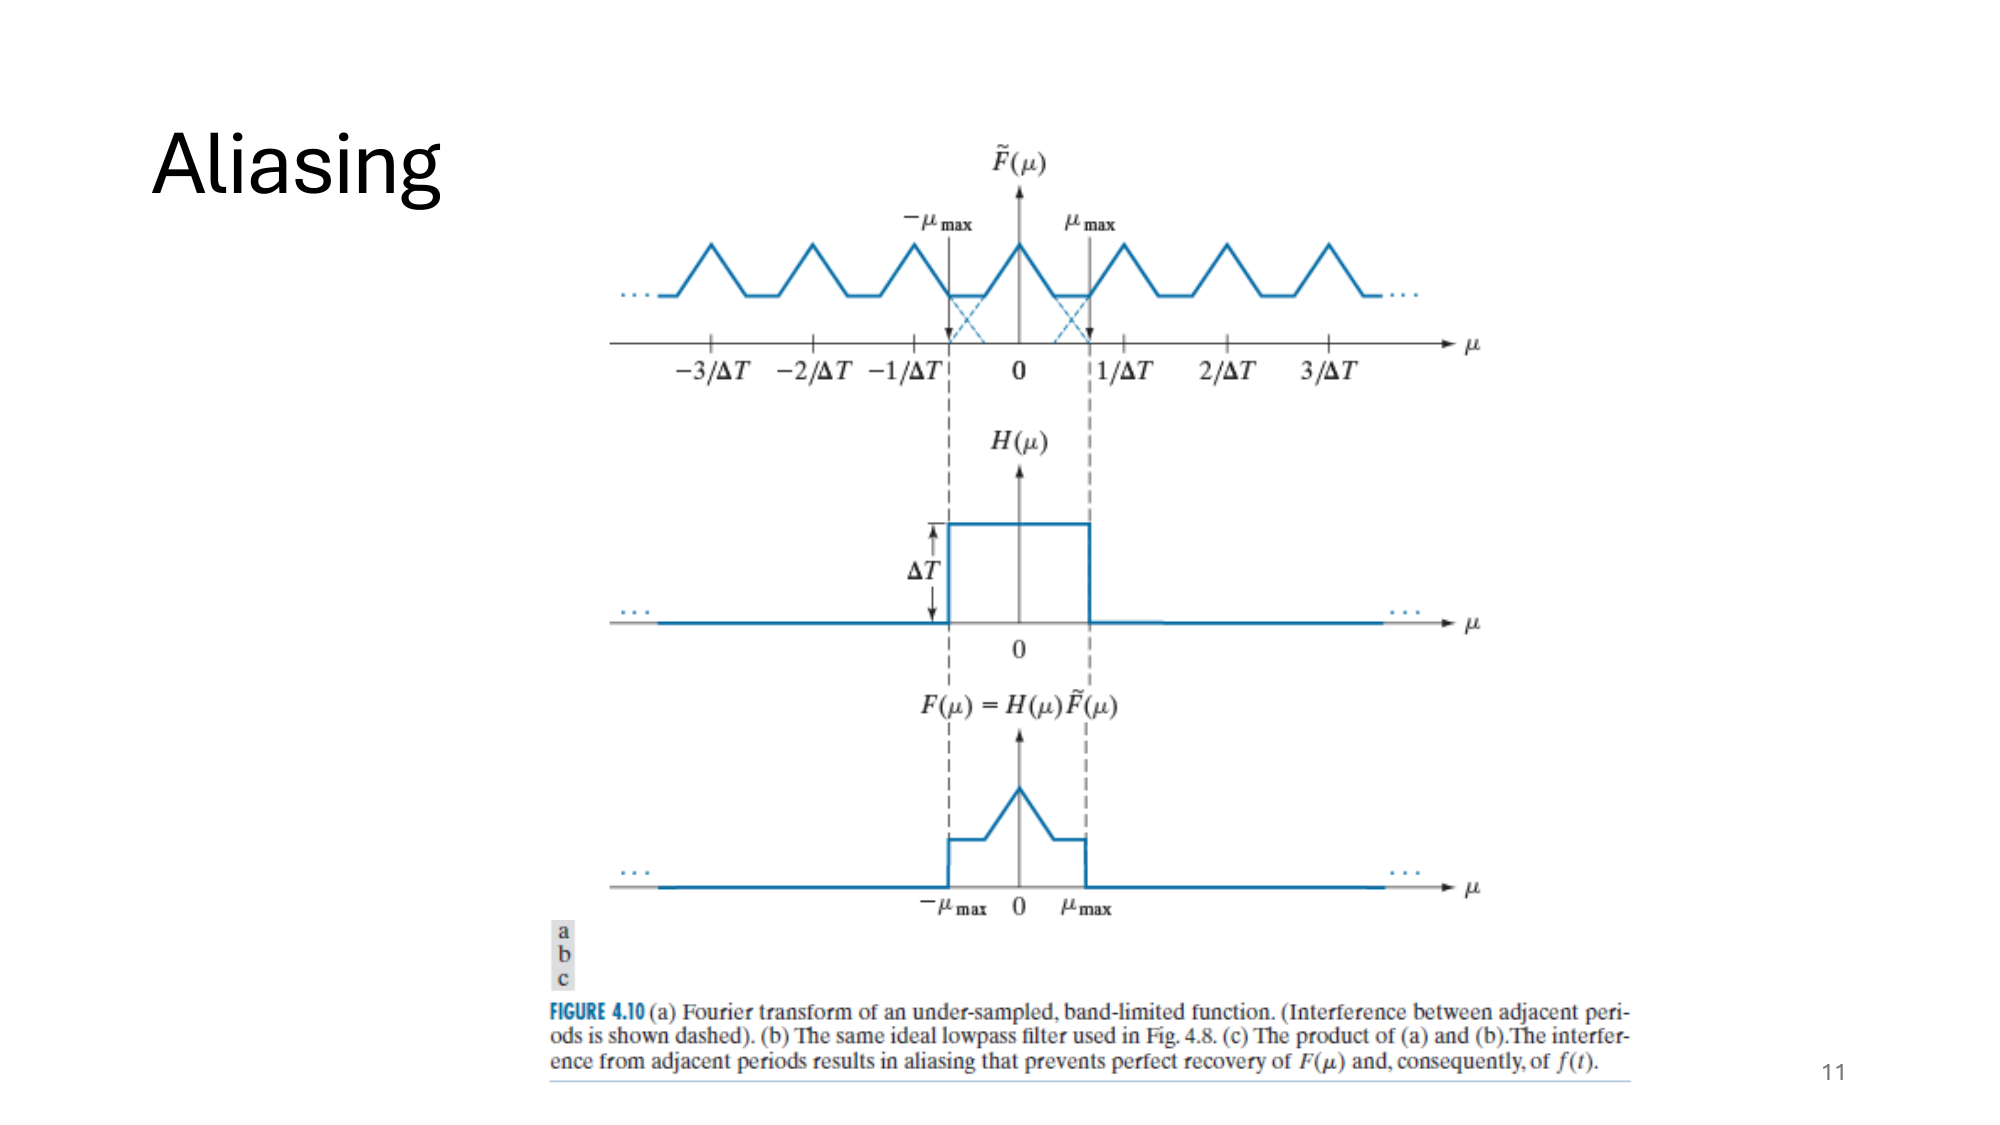
\includegraphics[width=0.85\textwidth]{images/slide8-11.png}
    \caption{Aliasing: spectrum overlap in undersampled signal prevents perfect recovery (FIGURE 4.10)}
    \label{fig:aliasing_spectrum}
\end{figure}

\begin{deepexplanation}
\textbf{DEEP ANALYSIS - Figure \ref{fig:aliasing_spectrum}: The Mechanism of Aliasing}

\textbf{When Does Aliasing Occur?}
When $f_s < 2f_{max}$, the spectrum copies are spaced closer than the signal bandwidth:
\[
\text{Copy spacing } f_s < 2f_{max} = \text{Signal bandwidth}
\]

\textbf{The Overlap Region:}
\begin{itemize}
    \item Baseband extends from $-f_{max}$ to $+f_{max}$
    \item First copy is centered at $f_s$, extending from $f_s - f_{max}$ to $f_s + f_{max}$
    \item If $f_s - f_{max} < f_{max}$ (i.e., $f_s < 2f_{max}$), the tail of the first copy invades the baseband region
\end{itemize}

\textbf{What Happens in the Overlap Region:}
The overlapping spectra \textbf{add together}. A frequency component originally at $f_{high}$ (where $f_{high} > f_s/2$) appears in the sampled signal as:
\[
f_{alias} = f_{high} - f_s \quad \text{or} \quad f_{alias} = f_s - f_{high}
\]
This ``aliased'' frequency is indistinguishable from a true low-frequency component.

\textbf{Why It's Irreversible:}
Once spectra overlap and add, you cannot separate them:
\begin{itemize}
    \item High frequency $f_1 = 800$ Hz sampled at $f_s = 1000$ Hz
    \item Creates alias at $f_{alias} = 1000 - 800 = 200$ Hz
    \item Original 200 Hz component + aliased 800 Hz component = combined, inseparable
\end{itemize}

\textbf{The Figure Illustrates:}
\begin{itemize}
    \item Spectrum copies overlapping at their tails
    \item The shaded overlap region where aliasing occurs
    \item High frequencies ``folding'' into low-frequency positions
\end{itemize}
\end{deepexplanation}

%==============================================================================
\section{Aliasing: Visual Manifestations}
%==============================================================================

\subsection{Aliasing in 1D Signals}

\begin{figure}[H]
    \centering
    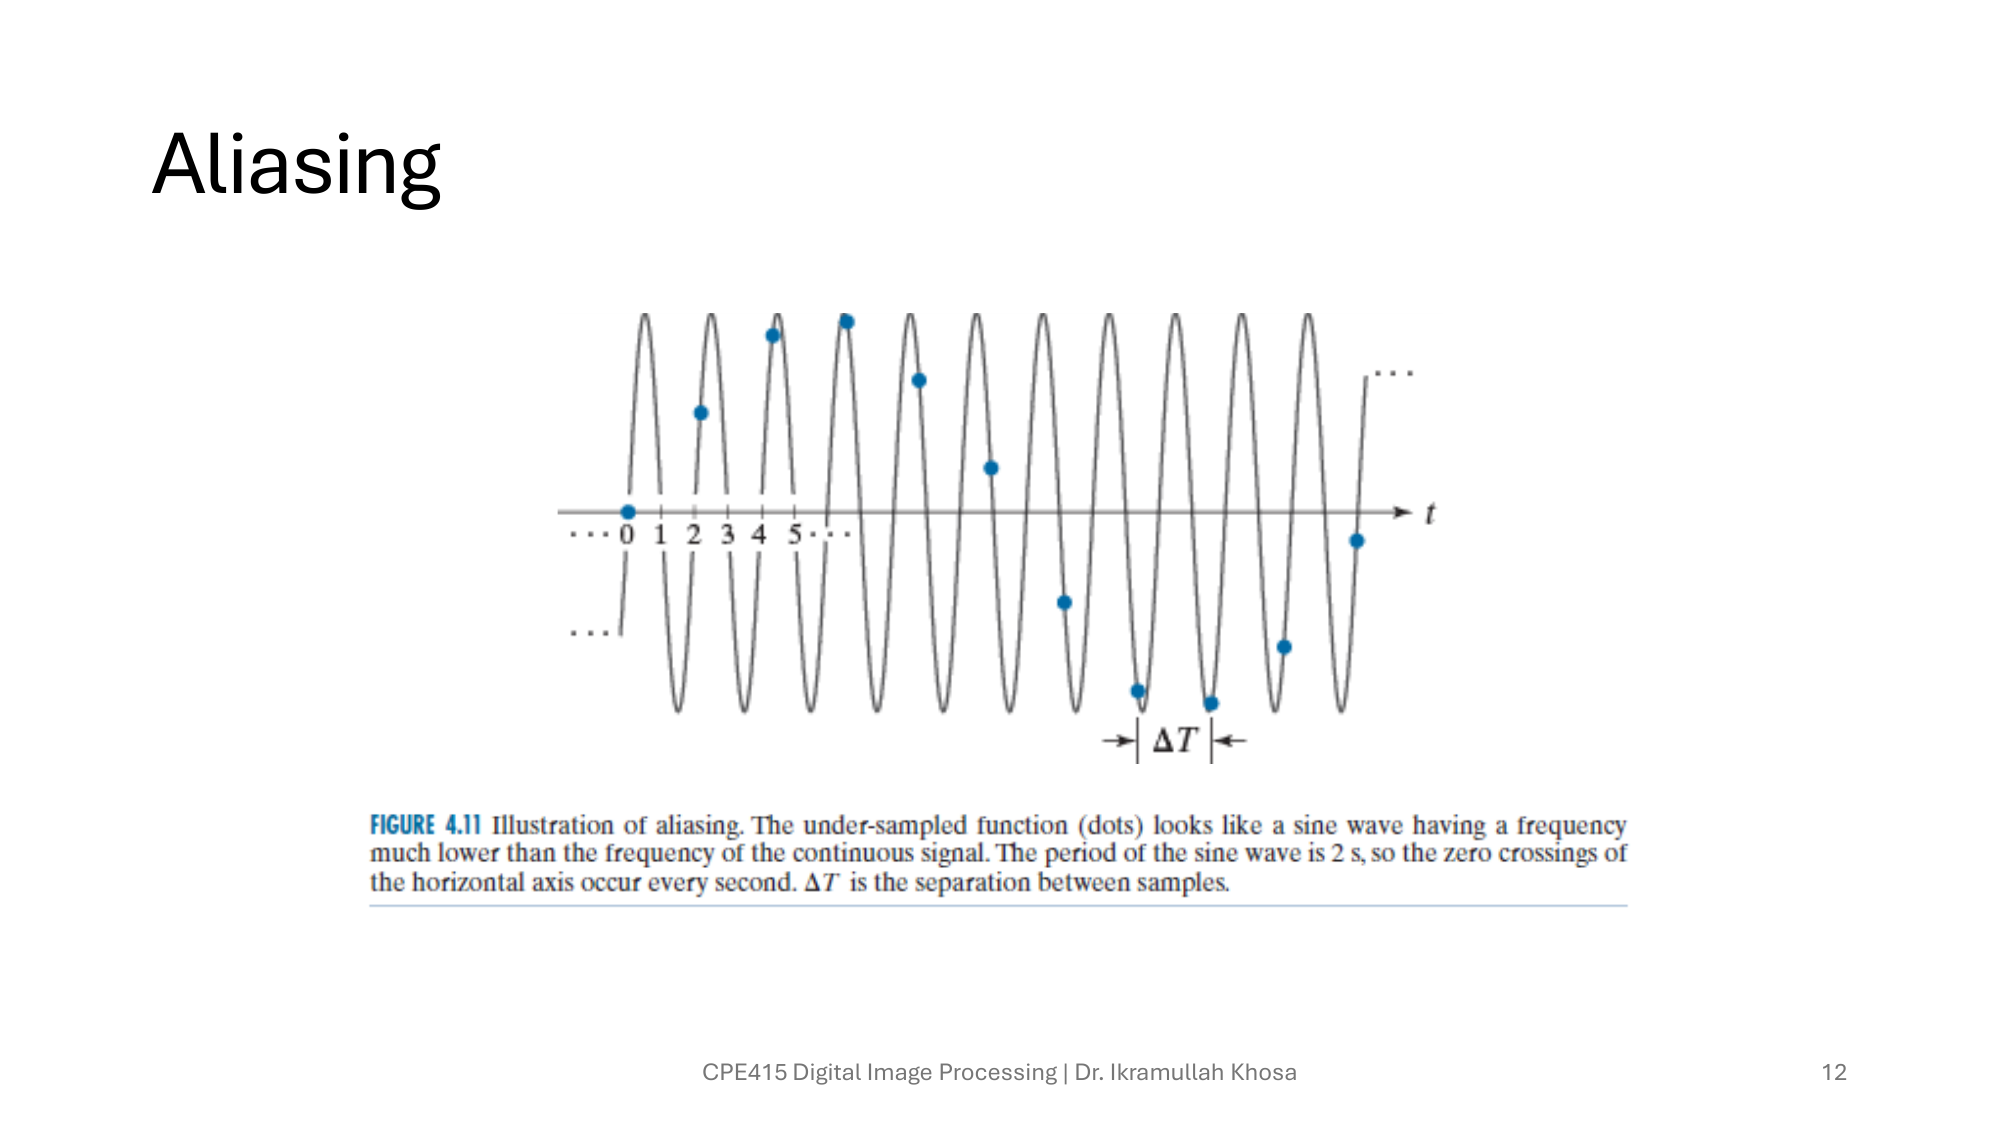
\includegraphics[width=0.85\textwidth]{images/slide8-12.png}
    \caption{Undersampled sine wave appears as lower frequency (FIGURE 4.11)}
    \label{fig:sine_aliasing}
\end{figure}

\begin{deepexplanation}
\textbf{DEEP ANALYSIS - Figure \ref{fig:sine_aliasing}: Seeing Aliasing in Action}

\textbf{The Classic Demonstration:}
Consider sampling a sine wave at frequency $f_{signal}$ with sampling rate $f_s$:

\textbf{Case 1: $f_s > 2f_{signal}$ (No aliasing)}
\begin{itemize}
    \item Samples accurately represent the sine wave
    \item Reconstruction recovers the original frequency
\end{itemize}

\textbf{Case 2: $f_s < 2f_{signal}$ (Aliasing)}
\begin{itemize}
    \item Samples appear to represent a \textbf{lower frequency} sine wave
    \item This false frequency is the ``alias''
\end{itemize}

\textbf{Mathematical Example:}
\begin{itemize}
    \item Signal: $\cos(2\pi \cdot 900 \cdot t)$ at 900 Hz
    \item Sampling: $f_s = 1000$ Hz (below Nyquist rate of 1800 Hz)
    \item Alias frequency: $|900 - 1000| = 100$ Hz
    \item The reconstructed signal appears to be a 100 Hz cosine!
\end{itemize}

\textbf{What the Figure Shows:}
\begin{enumerate}
    \item A high-frequency sine wave (many cycles)
    \item Sample points marked on this wave
    \item The same sample points connected by a lower-frequency sine
    \item The samples lie perfectly on both curves --- hence indistinguishable!
\end{enumerate}

\textbf{The Stroboscopic Effect (Real-World Analogy):}
This is why wagon wheels in movies appear to spin backward:
\begin{itemize}
    \item Wheel rotates at frequency $f_{wheel}$
    \item Camera captures at frame rate $f_{camera}$
    \item If $f_{wheel} > f_{camera}/2$, rotation appears slower or reversed
    \item At exactly $f_{wheel} = f_{camera}$, wheel appears stationary!
\end{itemize}
\end{deepexplanation}

\subsection{Aliasing in Images}

\begin{figure}[H]
    \centering
    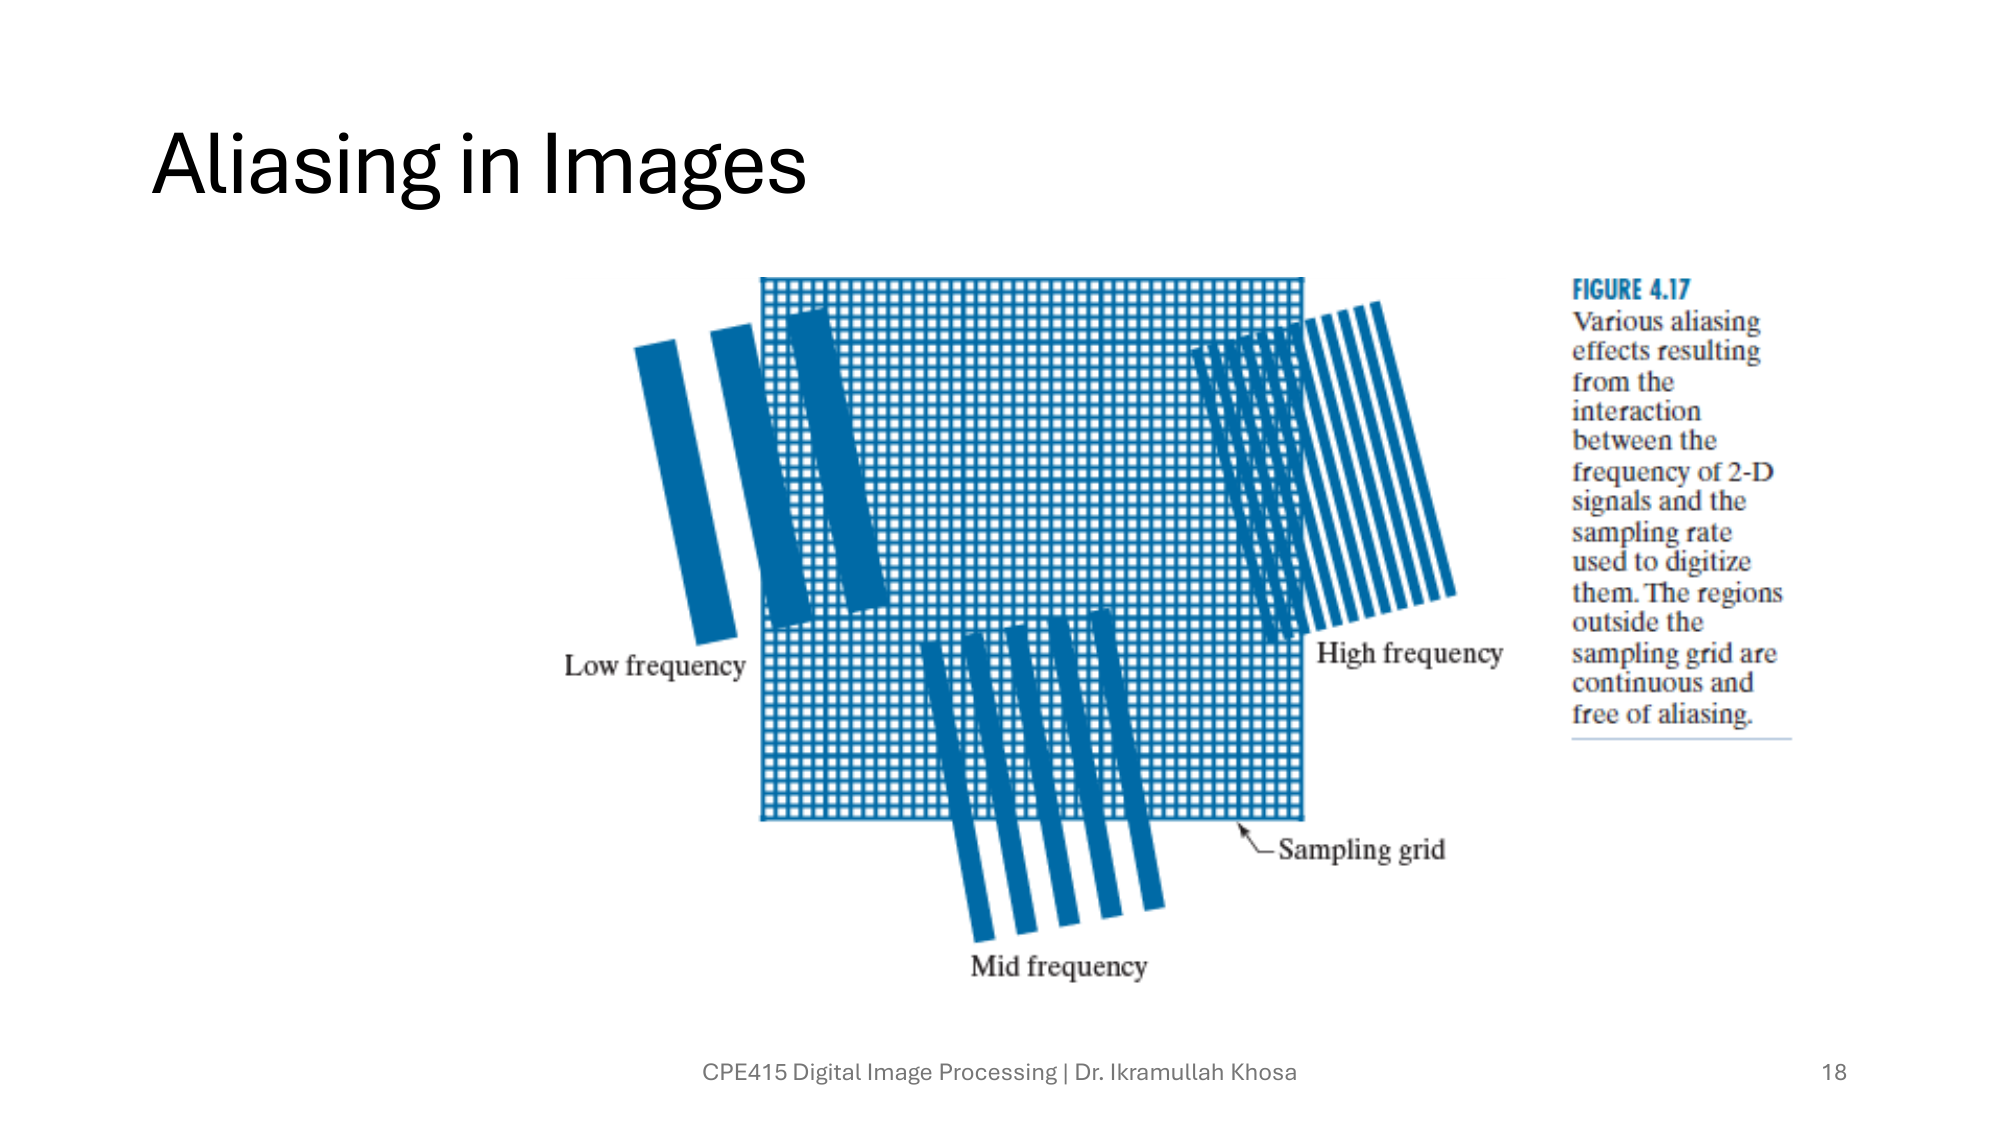
\includegraphics[width=0.9\textwidth]{images/slide8-18.png}
    \caption{Aliasing artifacts in images --- brick wall and fence examples}
    \label{fig:image_aliasing}
\end{figure}

\begin{deepexplanation}
\textbf{DEEP ANALYSIS - Figure \ref{fig:image_aliasing}: How Aliasing Creates Visible Artifacts}

\textbf{Why Images Are Susceptible:}
Images contain 2D spatial frequencies. A pattern with spacing $d$ has spatial frequency $f = 1/d$ cycles per unit length. When the pixel spacing $\Delta x$ doesn't satisfy $\Delta x < d/2$, aliasing occurs.

\textbf{Detailed Artifact Analysis:}

\textbf{1. Brick Wall Patterns:}
\begin{itemize}
    \item Bricks have regular spacing $d_{brick}$
    \item Camera pixel spacing creates sampling frequency $f_s = 1/\Delta_{pixel}$
    \item When $f_s < 2/d_{brick}$, the brick pattern aliases
    \item \textbf{Visual result}: Wavy, irregular patterns; false color fringes; patterns that ``swim'' as you zoom
    \item \textbf{Mechanism}: High-frequency brick edges fold into lower frequencies, creating beat frequencies with the pixel grid
\end{itemize}

\textbf{2. Fence/Railing Patterns:}
\begin{itemize}
    \item Vertical bars with spacing $d_{bar}$
    \item When $d_{bar}$ approaches pixel spacing, aliasing is severe
    \item \textbf{Visual result}: Bars appear to have varying thickness, merge together, or create zigzag patterns
    \item \textbf{Mechanism}: The bar frequency $f_{bar} = 1/d_{bar}$ aliases to $f_{alias} = |f_{bar} - f_s|$
\end{itemize}

\textbf{3. Fabric Textures:}
\begin{itemize}
    \item Woven patterns have characteristic frequencies
    \item \textbf{Visual result}: Shimmering rainbow colors (chromatic aliasing), moiré patterns
    \item \textbf{Mechanism}: Different color channels sample slightly differently, each aliasing to different frequencies
\end{itemize}

\textbf{The 2D Nature of Image Aliasing:}
Unlike 1D signals, images can alias in both $x$ and $y$ directions, plus diagonally. A diagonal line at angle $\theta$ has effective frequency $f_{diag} = f_x \cos\theta + f_y \sin\theta$, creating complex aliasing patterns.
\end{deepexplanation}

\begin{figure}[H]
    \centering
    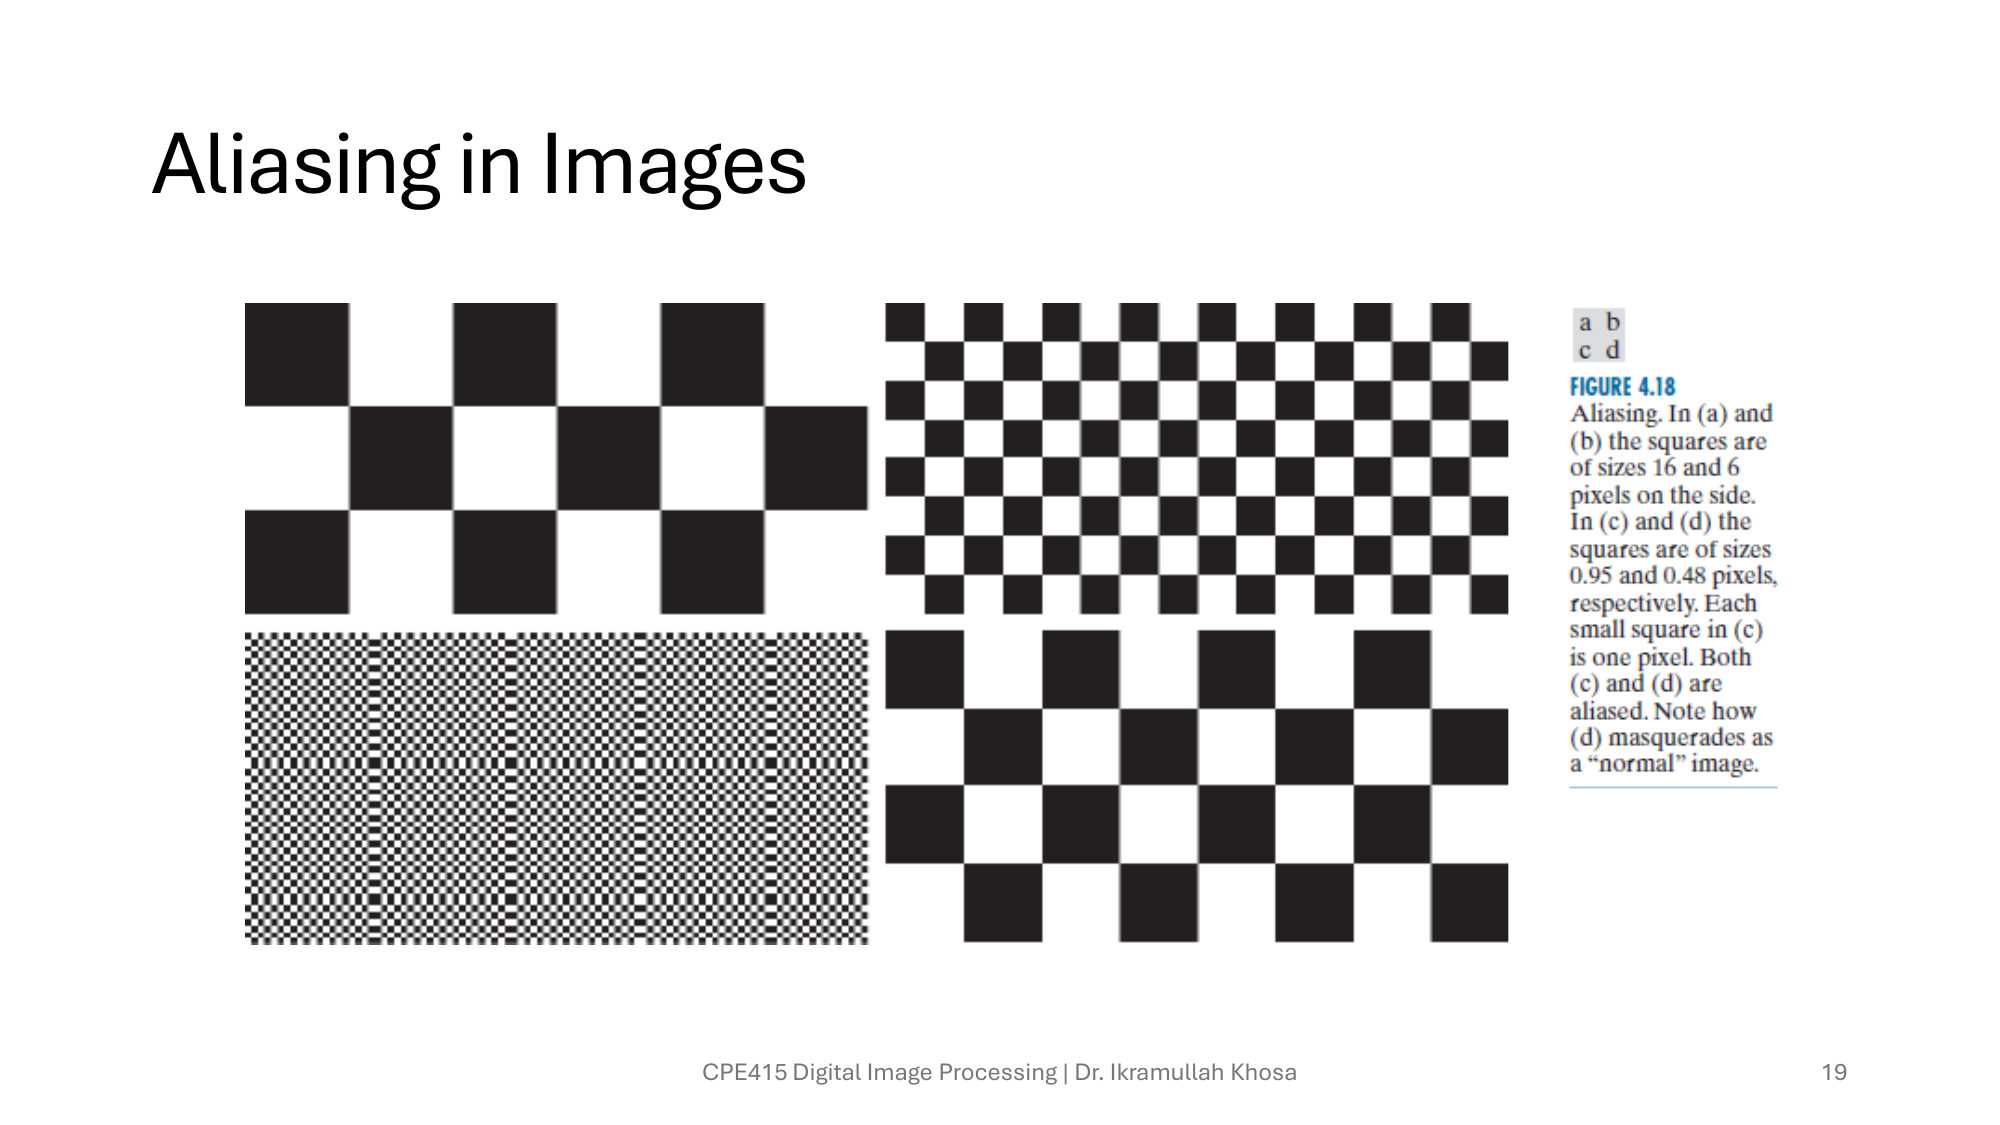
\includegraphics[width=0.9\textwidth]{images/slide8-19.png}
    \caption{More examples: Checkerboard aliasing and texture breakdown}
    \label{fig:image_aliasing2}
\end{figure}

\begin{deepexplanation}
\textbf{DEEP ANALYSIS - Figure \ref{fig:image_aliasing2}: Checkerboard and Texture Aliasing}

\textbf{Checkerboard Pattern Analysis:}
A perfect checkerboard has only one spatial frequency (plus harmonics):
\[
f_{checker} = \frac{1}{2 \times \text{square size}}
\]

\textbf{What Happens During Undersampling:}
\begin{enumerate}
    \item At sampling rate $f_s$, the checkerboard frequency $f_{checker}$ may exceed $f_s/2$
    \item The fundamental frequency aliases to $|f_{checker} - f_s|$
    \item Higher harmonics alias to other frequencies
    \item \textbf{Result}: The regular checkerboard becomes irregular blobs, waves, or noise-like patterns
\end{enumerate}

\textbf{Zone Plate Demonstration:}
A zone plate (circular pattern with increasing frequency toward the edge) is the perfect aliasing test:
\begin{itemize}
    \item Center: Low frequency, properly sampled
    \item Edge: High frequency, aliased
    \item Visible transition: The radius where frequency exceeds Nyquist
    \item Beyond transition: Apparent frequency \textbf{decreases} (frequency folds back)
\end{itemize}

\textbf{Texture Breakdown Analysis:}
Fine textures (grass, hair, fabric) contain broad spectrum:
\begin{itemize}
    \item Frequencies below Nyquist: Preserved correctly
    \item Frequencies above Nyquist: Alias into lower frequencies
    \item \textbf{Result}: False patterns emerge where texture should appear random
    \item Particularly visible in video: Aliased patterns shift frame-to-frame, creating ``crawling'' or ``buzzing'' effects
\end{itemize}

\textbf{Why Side-by-Side Comparisons Are Revealing:}
\begin{itemize}
    \item Properly sampled/anti-aliased image: Smooth, possibly blurry in high-frequency areas
    \item Aliased image: Sharp but with false patterns
    \item The aliased version may look ``sharper'' but contains incorrect information
\end{itemize}
\end{deepexplanation}

\begin{figure}[H]
    \centering
    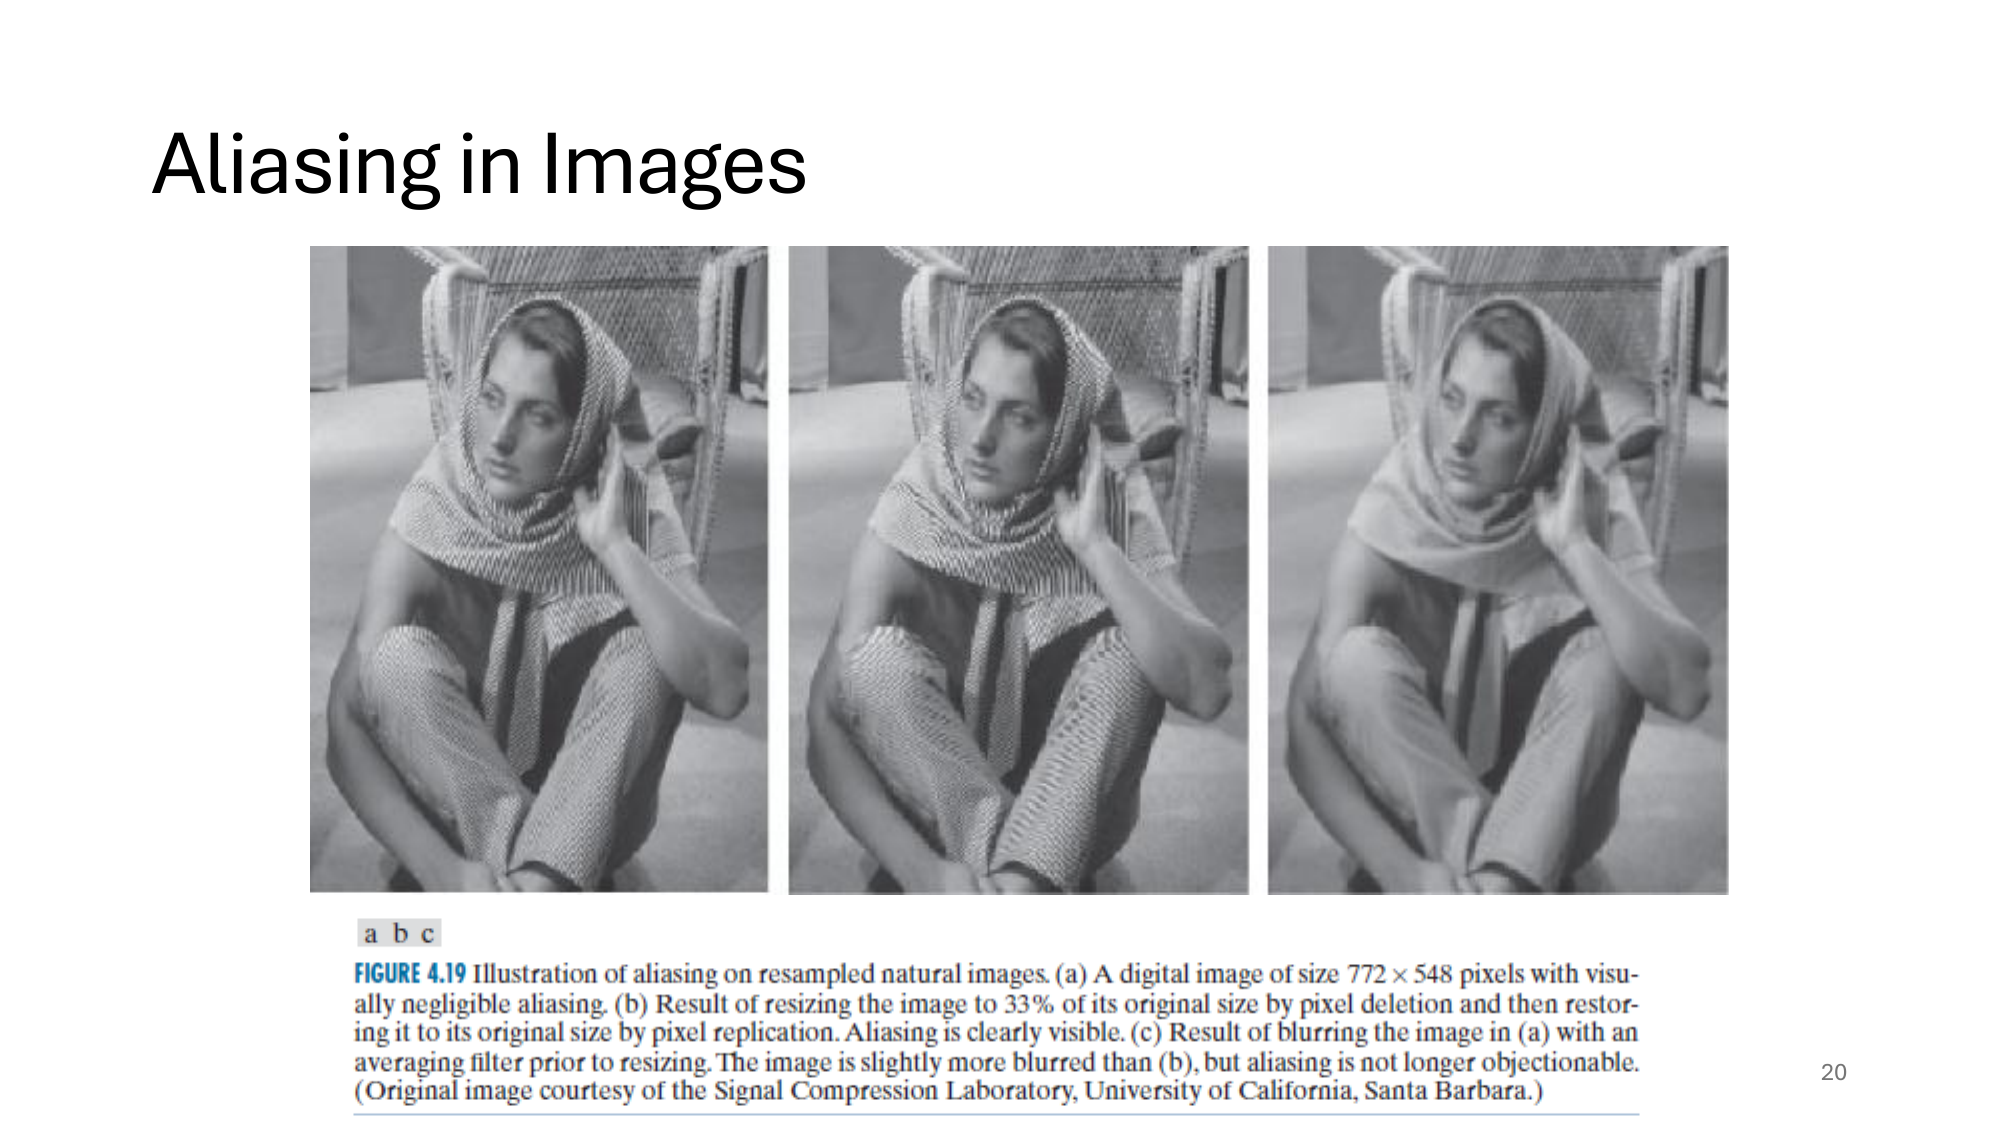
\includegraphics[width=0.95\textwidth]{images/slide8-20.png}
    \caption{Aliasing on resampled natural images --- comparing proper vs.\ improper downsampling (FIGURE 4.19)}
    \label{fig:aliasing_natural}
\end{figure}

\begin{deepexplanation}
\textbf{DEEP ANALYSIS - Figure \ref{fig:aliasing_natural}: Aliasing in Natural Image Resampling}

\textbf{What This Figure Shows:}
A classic demonstration using a 772$\times$548 pixel image resized to 33\% then back to original size using two methods:
\begin{itemize}
    \item \textbf{(a)} Original image: Full resolution with minimal aliasing
    \item \textbf{(b)} Downsampled by pixel deletion, then upsampled by pixel replication: \textbf{Strong aliasing visible}
    \item \textbf{(c)} Anti-aliased with averaging filter before downsampling: \textbf{No aliasing, slightly blurry}
\end{itemize}

\textbf{Why Pixel Deletion Causes Aliasing:}
When you reduce image size by simply deleting pixels:
\begin{itemize}
    \item High-frequency content (fine textures, edges) exceeds the new Nyquist limit
    \item These frequencies ``fold back'' into lower frequencies
    \item In the woven basket and headscarf, regular patterns create false moiré-like artifacts
    \item The stair-stepping on edges (jaggies) is a form of spatial aliasing
\end{itemize}

\textbf{The Correct Approach (Anti-Aliasing):}
Before downsampling:
\begin{enumerate}
    \item Apply a \textbf{lowpass filter} (averaging or Gaussian blur)
    \item This removes frequencies above the new Nyquist limit
    \item Then perform subsampling (pixel deletion)
    \item Result: Slightly softer but artifact-free image
\end{enumerate}

\textbf{Mathematical Justification:}
\[
\text{If } f_{\text{original}} > \frac{f_{\text{new}}}{2}, \text{ aliasing occurs}
\]
The averaging filter acts as a lowpass filter with cutoff $\approx f_{\text{new}}/2$, preventing aliasing.

\textbf{Practical Applications:}
\begin{itemize}
    \item \textbf{Image thumbnails}: Always anti-alias before shrinking
    \item \textbf{Video downscaling}: Progressive scaling with filtering
    \item \textbf{Mipmap generation}: Pre-filtered texture levels in 3D graphics
    \item \textbf{Photo editing}: Quality settings control anti-aliasing filter strength
\end{itemize}
\end{deepexplanation}

\subsection{Moiré Patterns}

Moiré patterns are a specific type of aliasing that occurs when two regular patterns interfere.

\begin{figure}[H]
    \centering
    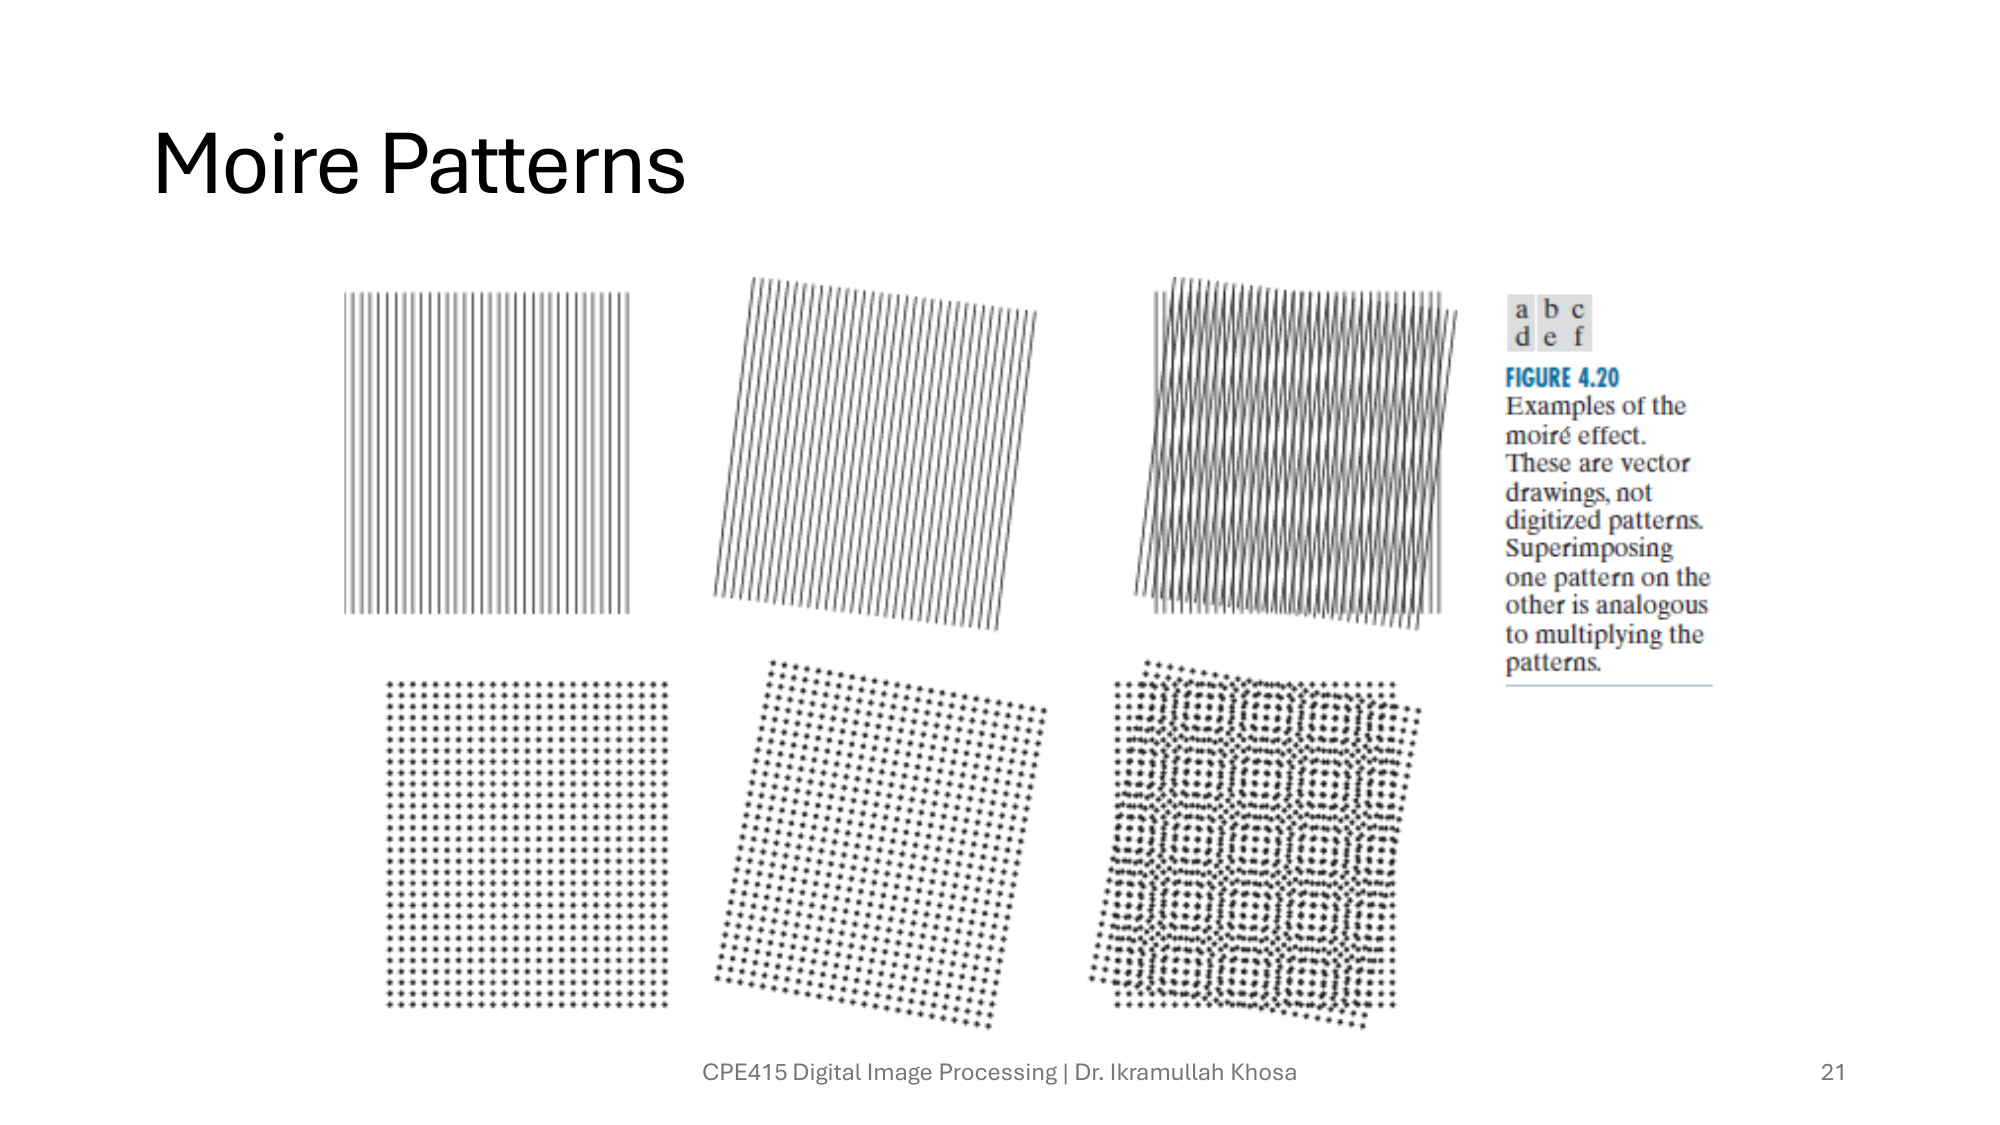
\includegraphics[width=0.85\textwidth]{images/slide8-21.png}
    \caption{Moiré pattern formation from overlapping periodic structures (FIGURE 4.20)}
    \label{fig:moire1}
\end{figure}

\begin{deepexplanation}
\textbf{DEEP ANALYSIS - Figure \ref{fig:moire1}: The Mathematics of Moiré Patterns}

\textbf{What This Figure Shows:}
This classic demonstration uses vector-drawn patterns (not digitized images) to illustrate the moiré effect in its purest form:
\begin{itemize}
    \item \textbf{Top row (a, b, c)}: Line gratings --- vertical lines at different angles, and their superposition
    \item \textbf{Bottom row (d, e, f)}: Dot patterns --- regular dot arrays at different angles, and their overlay
\end{itemize}

\textbf{How Moiré Patterns Form:}
When two periodic patterns with slightly different frequencies or orientations overlap, they create a beat frequency:
\[
f_{moire} = |f_1 - f_2|
\]

\textbf{Detailed Mechanism:}
Consider two gratings (line patterns):
\begin{itemize}
    \item Grating 1: Lines spaced $d_1$ apart, frequency $f_1 = 1/d_1$
    \item Grating 2: Lines spaced $d_2$ apart, frequency $f_2 = 1/d_2$
    \item Overlay transmission: $T(x) \propto \cos(2\pi f_1 x) \cdot \cos(2\pi f_2 x)$
\end{itemize}

Using the product-to-sum identity:
\[
\cos(A)\cos(B) = \frac{1}{2}[\cos(A-B) + \cos(A+B)]
\]

The result contains:
\begin{itemize}
    \item Difference frequency: $|f_1 - f_2|$ (low-frequency moiré pattern)
    \item Sum frequency: $f_1 + f_2$ (high frequency, often invisible)
\end{itemize}

\textbf{Angular Moiré (shown in figure):}
When two identical gratings are rotated by angle $\theta$:
\[
\text{Moiré spacing} = \frac{d}{2\sin(\theta/2)}
\]
Even a small angle creates large-scale visible patterns!

\textbf{What Each Panel Demonstrates:}
\begin{itemize}
    \item \textbf{(a, d)}: Single pattern --- no moiré
    \item \textbf{(b, e)}: Same pattern rotated --- still no moiré alone
    \item \textbf{(c, f)}: Superposition creates dramatic low-frequency moiré fringes
\end{itemize}
\end{deepexplanation}

\begin{figure}[H]
    \centering
    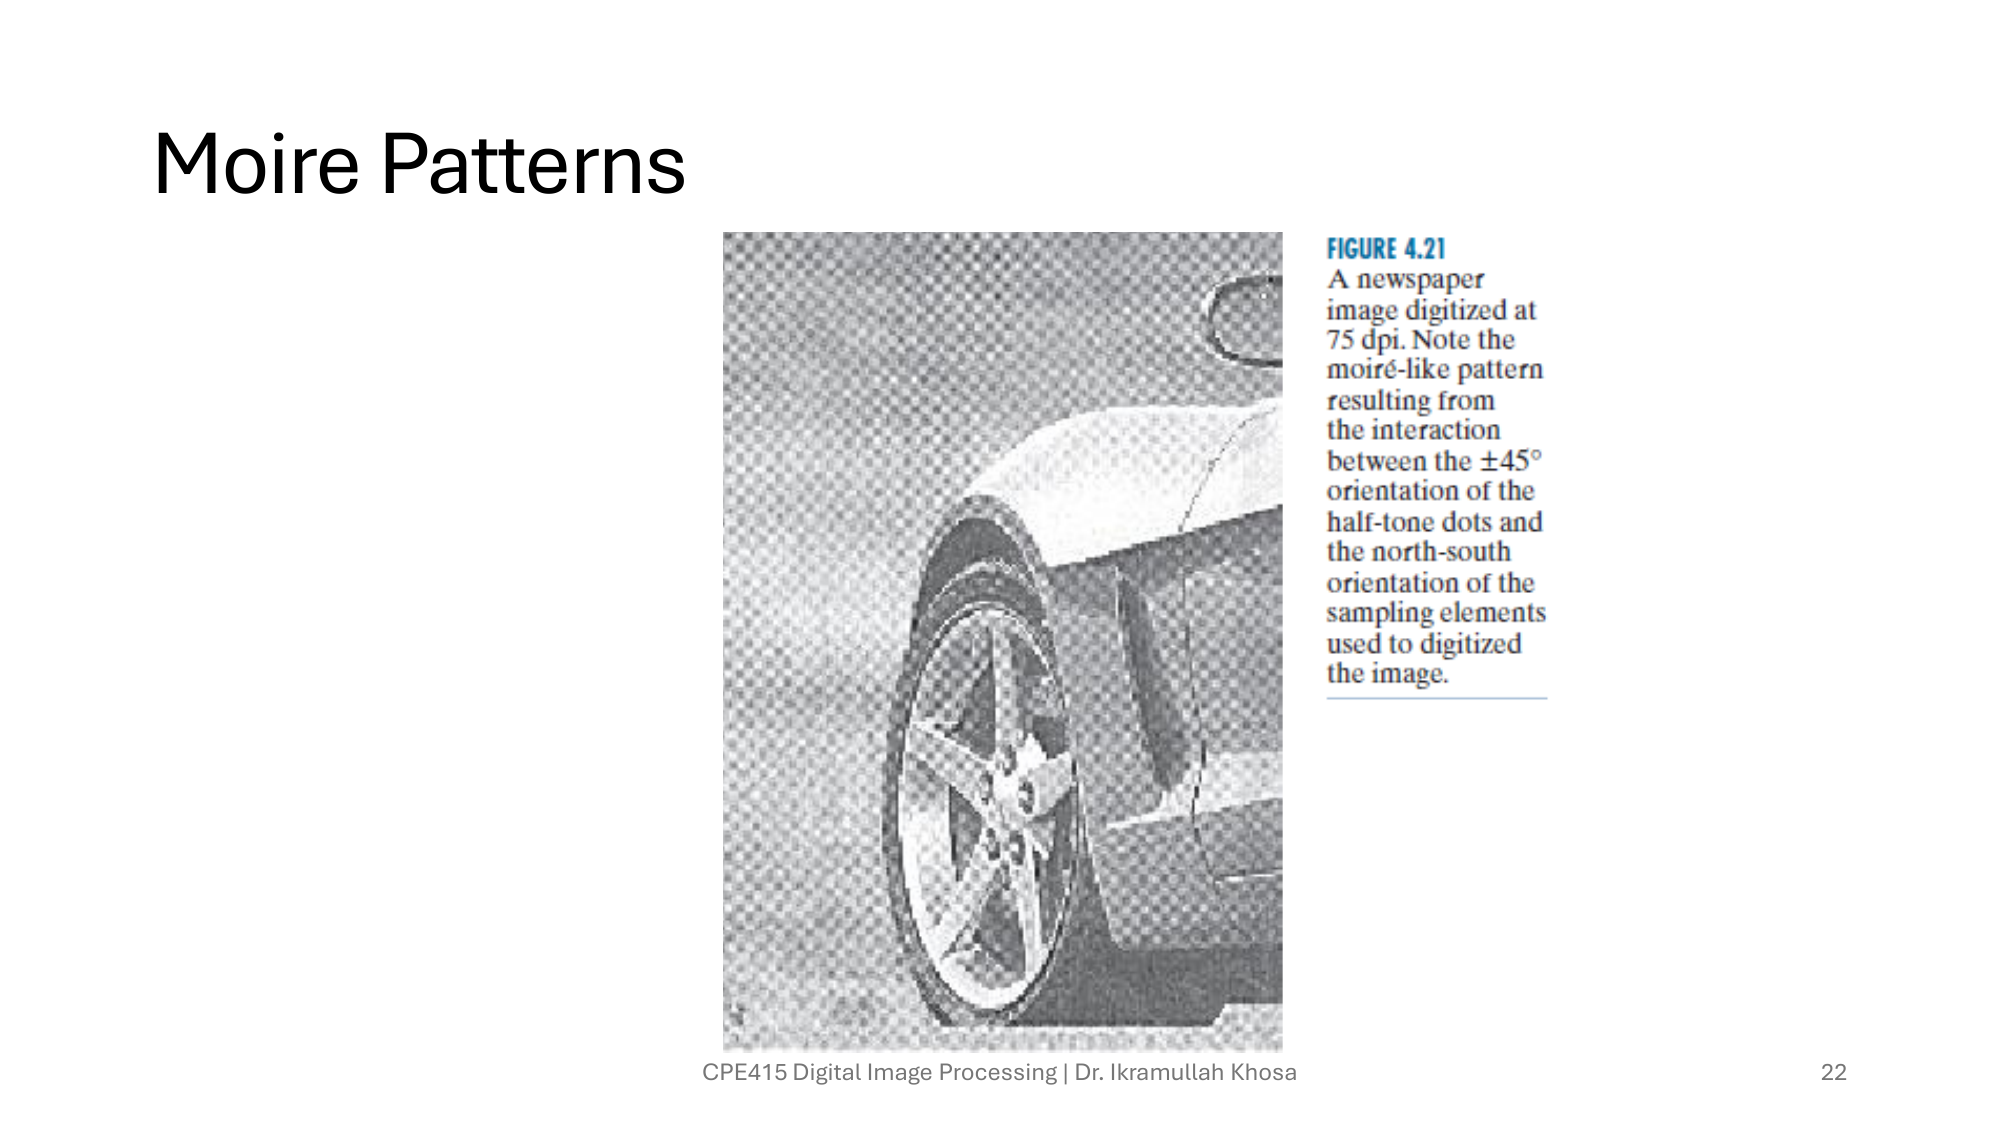
\includegraphics[width=0.85\textwidth]{images/slide8-22.png}
    \caption{Moiré patterns in newspaper halftone digitization (FIGURE 4.21)}
    \label{fig:moire2}
\end{figure}

\begin{deepexplanation}
\textbf{DEEP ANALYSIS - Figure \ref{fig:moire2}: Moiré in Newspaper Digitization (FIGURE 4.21)}

\textbf{What This Figure Shows:}
A newspaper image (car photograph) digitized at 75 dpi, exhibiting strong moiré patterns. The visible interference comes from the interaction between:
\begin{itemize}
    \item The halftone dot pattern used in newspaper printing ($\pm 45°$ orientation)
    \item The rectangular sampling grid of the scanner (north-south aligned)
\end{itemize}

\textbf{Why Halftone Printing Creates This Problem:}
Newspapers print continuous-tone images using \textbf{halftoning}:
\begin{itemize}
    \item Tiny dots of ink at regular spacing (screen ruling)
    \item Dot size varies to create the illusion of gray levels
    \item Standard newspaper: 65--85 lines per inch (lpi)
    \item Dots are typically oriented at $45°$ to make them less visible
\end{itemize}

\textbf{The Moiré Mechanism:}
When digitizing at 75 dpi with a 75 lpi halftone screen:
\begin{itemize}
    \item Scanner sampling frequency $\approx$ halftone frequency
    \item The $\pm 45°$ dot orientation vs. $0°/90°$ pixel grid creates angular moiré
    \item Result: Large-scale wavy patterns superimposed on the image
\end{itemize}

\textbf{Mathematical Analysis:}
\[
\text{Moiré period} = \frac{d}{2\sin(\theta/2)} \quad \text{where } \theta = 45° \text{ and } d \approx \text{dot spacing}
\]

\textbf{Solutions for Halftone Moiré:}
\begin{itemize}
    \item \textbf{Higher resolution scanning}: Sample at 2--4$\times$ the halftone frequency
    \item \textbf{Descreen filters}: Lowpass filtering before resampling
    \item \textbf{Slight defocus}: Optical anti-aliasing
    \item \textbf{Rotation}: Tilt the original slightly during scanning
\end{itemize}
\end{deepexplanation}


%==============================================================================
\section{2D Fourier Transform for Images}
%==============================================================================

\subsection{Extension to Two Dimensions}

For images, we extend the Fourier transform to 2D:

\begin{mathbox}
\textbf{2D Continuous Fourier Transform:}
\[
F(u, v) = \int_{-\infty}^{\infty} \int_{-\infty}^{\infty} f(x, y) e^{-j2\pi(ux + vy)} \, dx \, dy
\]
\textbf{Inverse:}
\[
f(x, y) = \int_{-\infty}^{\infty} \int_{-\infty}^{\infty} F(u, v) e^{j2\pi(ux + vy)} \, du \, dv
\]
\end{mathbox}

\subsection{2D Impulse and Sampling}

\begin{figure}[H]
    \centering
    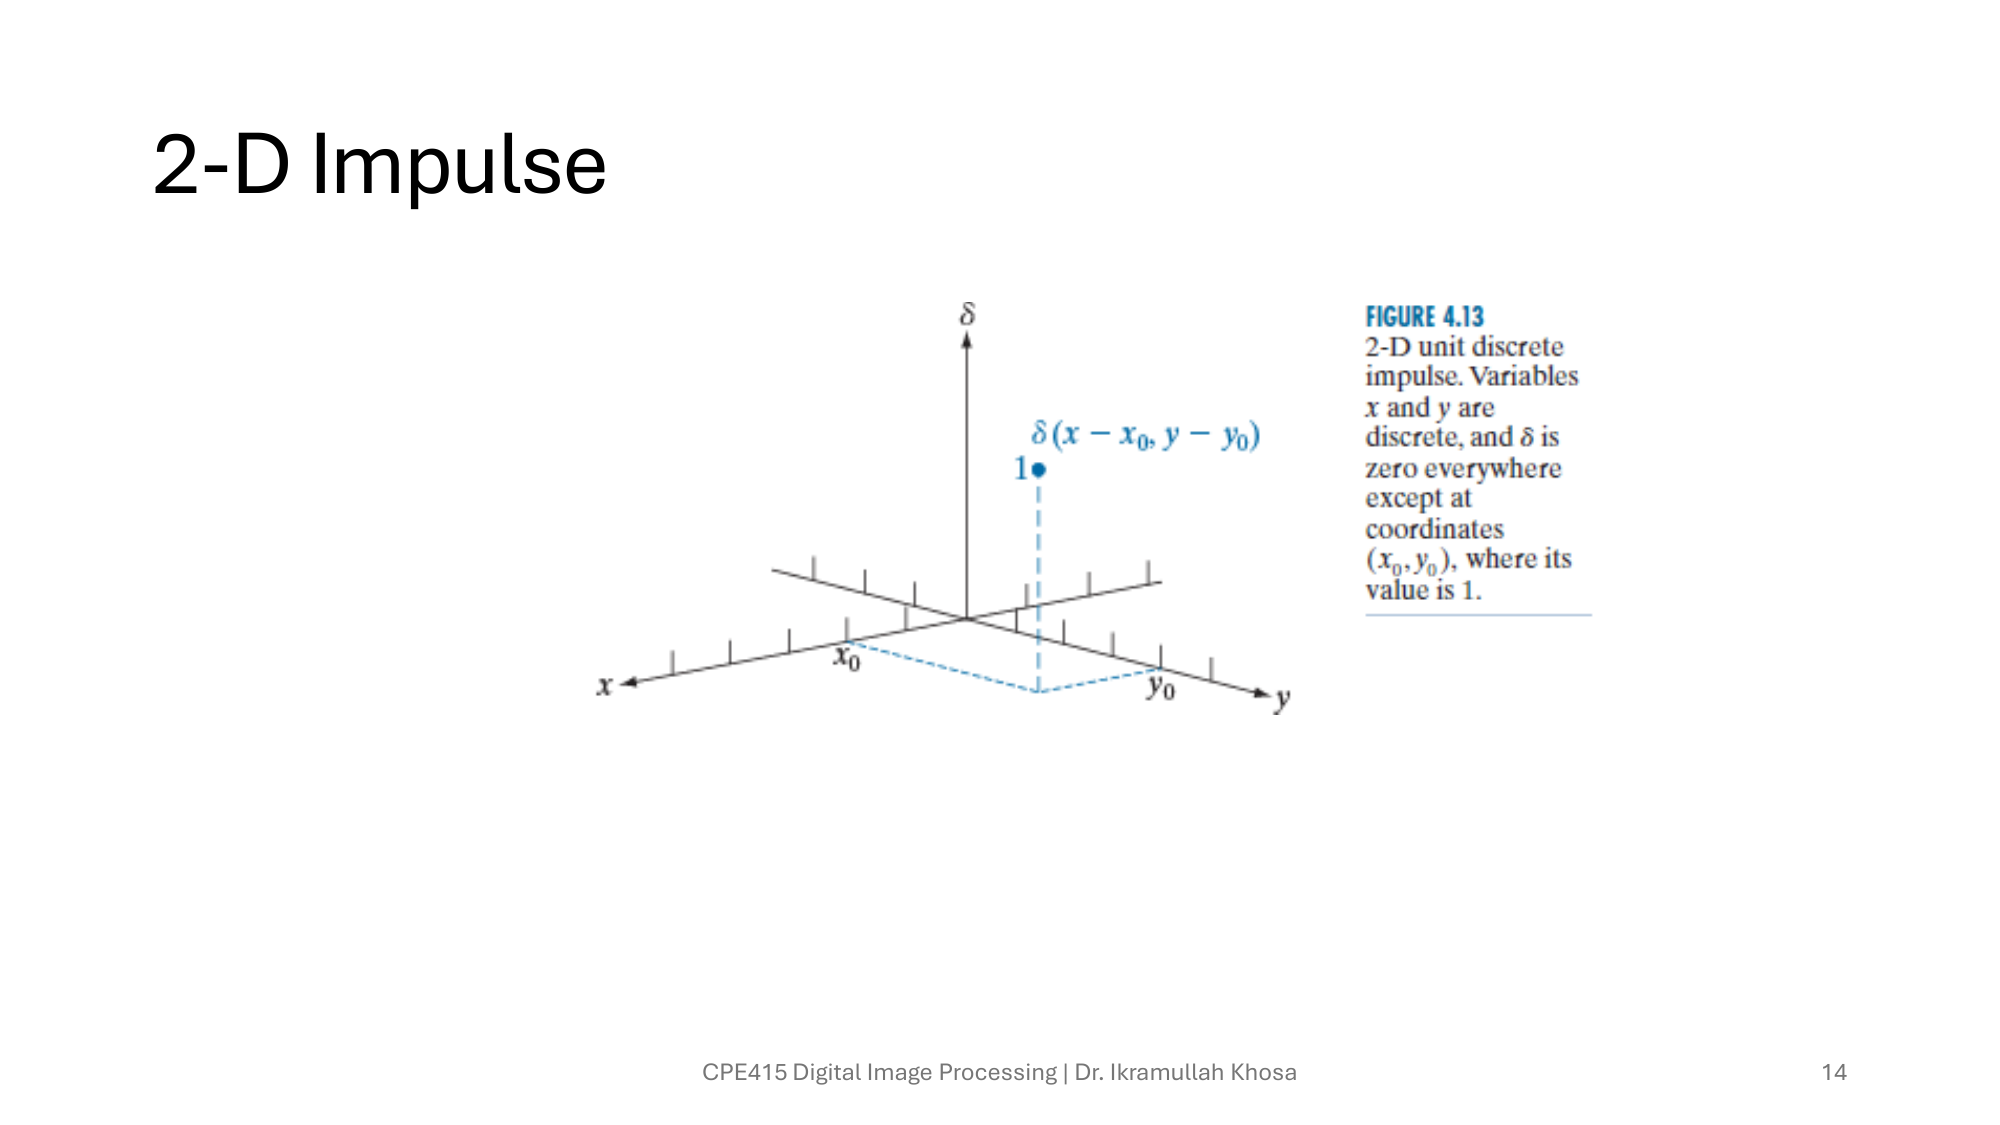
\includegraphics[width=0.7\textwidth]{images/slide8-14.png}
    \caption{2D impulse function visualization}
    \label{fig:2d_impulse}
\end{figure}

\begin{deepexplanation}
\textbf{DEEP ANALYSIS - Figure \ref{fig:2d_impulse}: The 2D Dirac Delta Function}

\textbf{Mathematical Definition:}
\[
\delta(x, y) = \begin{cases} \infty & x = 0 \text{ and } y = 0 \\ 0 & \text{otherwise} \end{cases}
\]
with
\[
\int_{-\infty}^{\infty} \int_{-\infty}^{\infty} \delta(x, y) \, dx \, dy = 1
\]

\textbf{2D Sifting Property:}
\[
\int_{-\infty}^{\infty} \int_{-\infty}^{\infty} f(x, y) \delta(x - x_0, y - y_0) \, dx \, dy = f(x_0, y_0)
\]

\textbf{What the Figure Shows:}
\begin{itemize}
    \item A 3D plot with the $x$-$y$ plane as the base
    \item A single infinitely tall spike at the origin
    \item Often visualized as an arrow or a very narrow, tall peak
\end{itemize}

\textbf{Physical Interpretation for Images:}
\begin{itemize}
    \item Represents a single ``point'' of light at location $(x_0, y_0)$
    \item In digital images: Approximated by a single white pixel on a black background
    \item The image of a perfect point source through an optical system reveals the system's Point Spread Function (PSF)
\end{itemize}

\textbf{Fourier Transform:}
\[
\mathcal{F}\{\delta(x, y)\} = 1 \quad \text{(constant across all frequencies)}
\]
A perfect point contains all spatial frequencies equally --- it's the ultimate ``sharp'' feature.
\end{deepexplanation}

\begin{figure}[H]
    \centering
    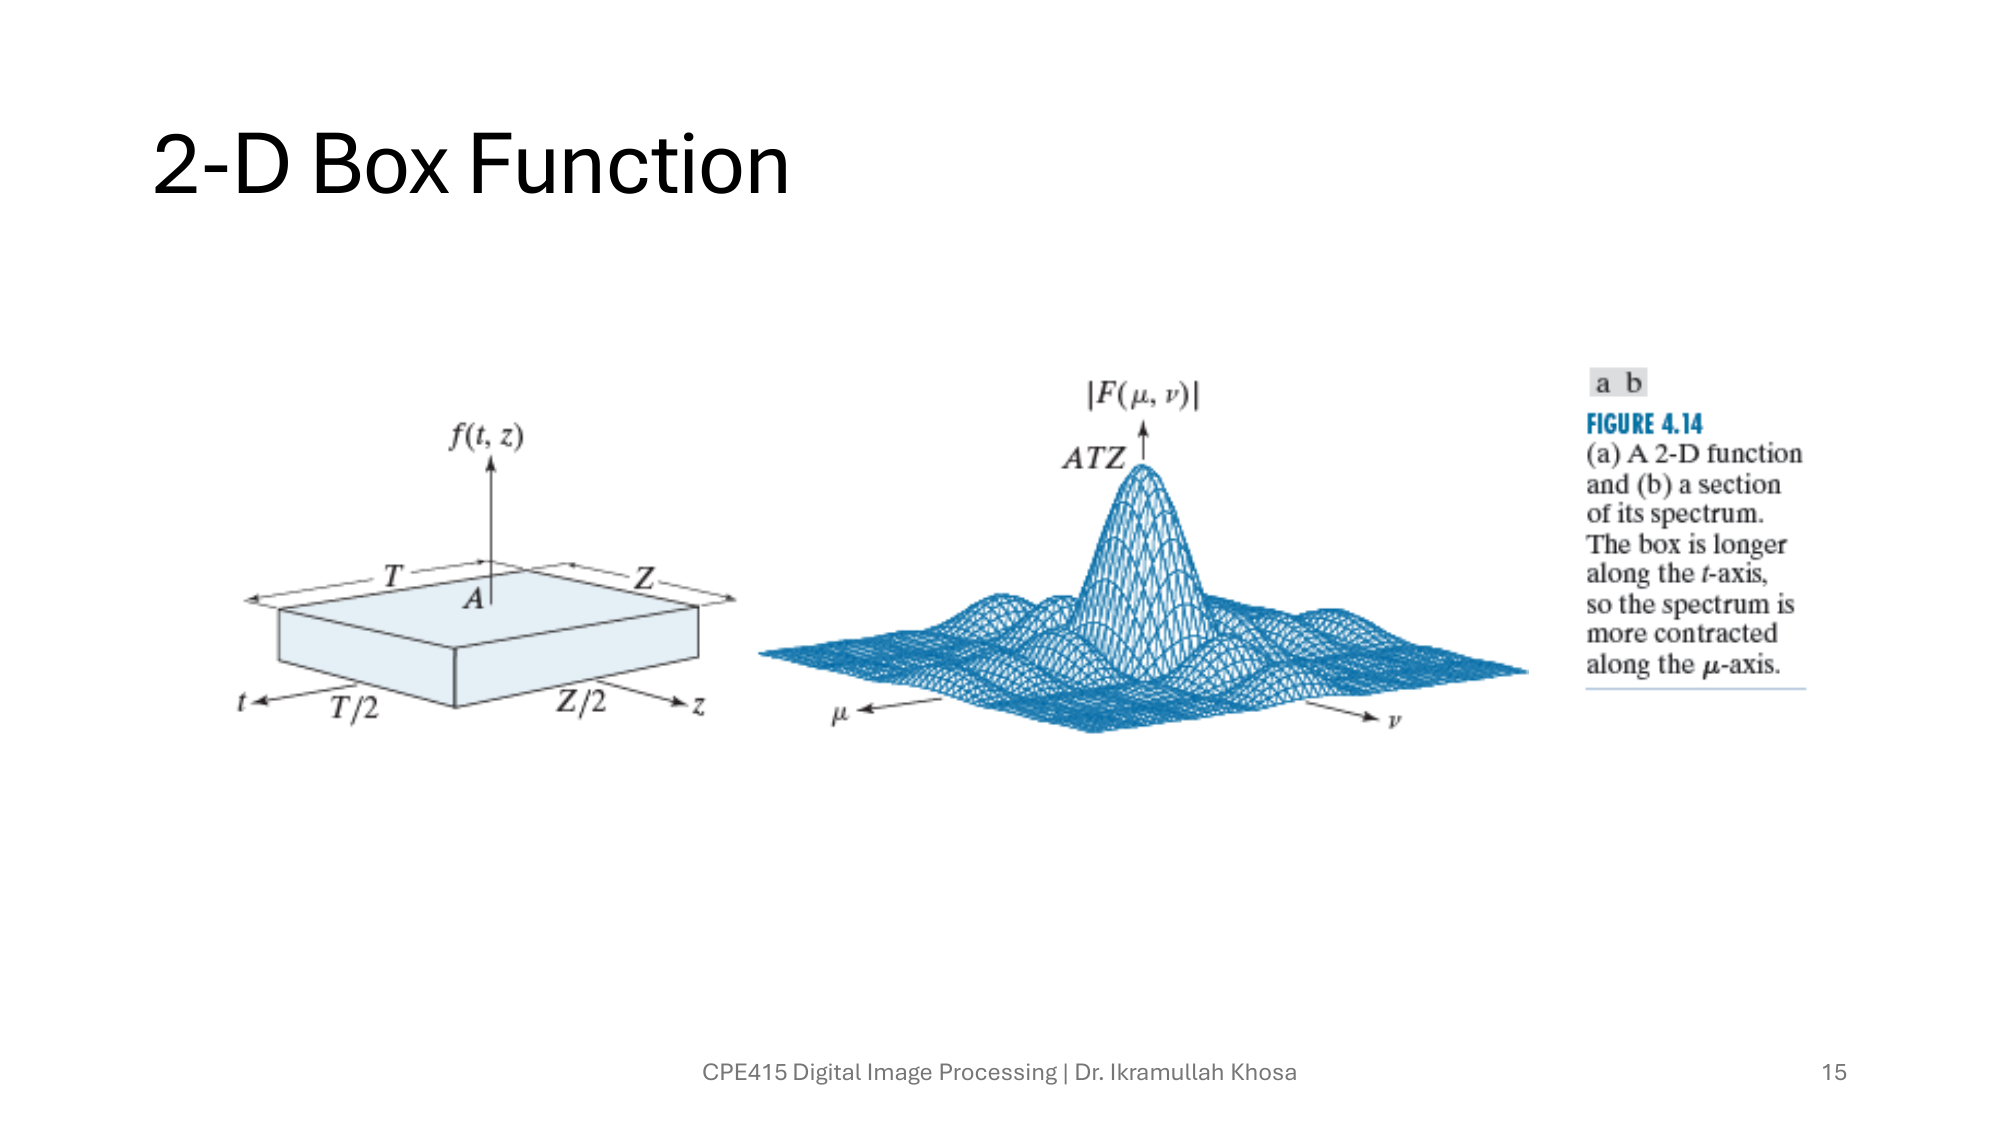
\includegraphics[width=0.7\textwidth]{images/slide8-15.png}
    \caption{2D box function and its transform}
    \label{fig:2d_box}
\end{figure}

\begin{deepexplanation}
\textbf{DEEP ANALYSIS - Figure \ref{fig:2d_box}: The 2D Rectangle Function}

\textbf{Definition:}
\[
\text{rect}(x/W, y/H) = \begin{cases} 1 & |x| \leq W/2 \text{ and } |y| \leq H/2 \\ 0 & \text{otherwise} \end{cases}
\]

\textbf{Fourier Transform:}
\[
\mathcal{F}\{\text{rect}(x/W, y/H)\} = WH \cdot \text{sinc}(Wu) \cdot \text{sinc}(Hv)
\]

The transform is \textbf{separable} --- the 2D result is the product of two 1D results.

\textbf{What the Figure Shows:}
\begin{itemize}
    \item A flat rectangular region with constant value (often normalized to 1)
    \item Sharp edges at $x = \pm W/2$ and $y = \pm H/2$
    \item The corresponding 2D sinc pattern in frequency domain
\end{itemize}

\textbf{Frequency Domain Characteristics:}
\begin{itemize}
    \item Central peak (DC component) proportional to the rectangle's area
    \item Ripples extending in both $u$ and $v$ directions
    \item Zero crossings at $u = \pm n/W$ and $v = \pm m/H$
    \item The sharp spatial edges create infinite frequency ripples
\end{itemize}

\textbf{Practical Significance:}
\begin{itemize}
    \item Rectangular truncation of images (windowing) introduces this sinc pattern
    \item Ideal 2D lowpass filter = rectangle in frequency = 2D sinc in space
    \item Ringing artifacts near image edges come from this relationship
\end{itemize}
\end{deepexplanation}

\begin{figure}[H]
    \centering
    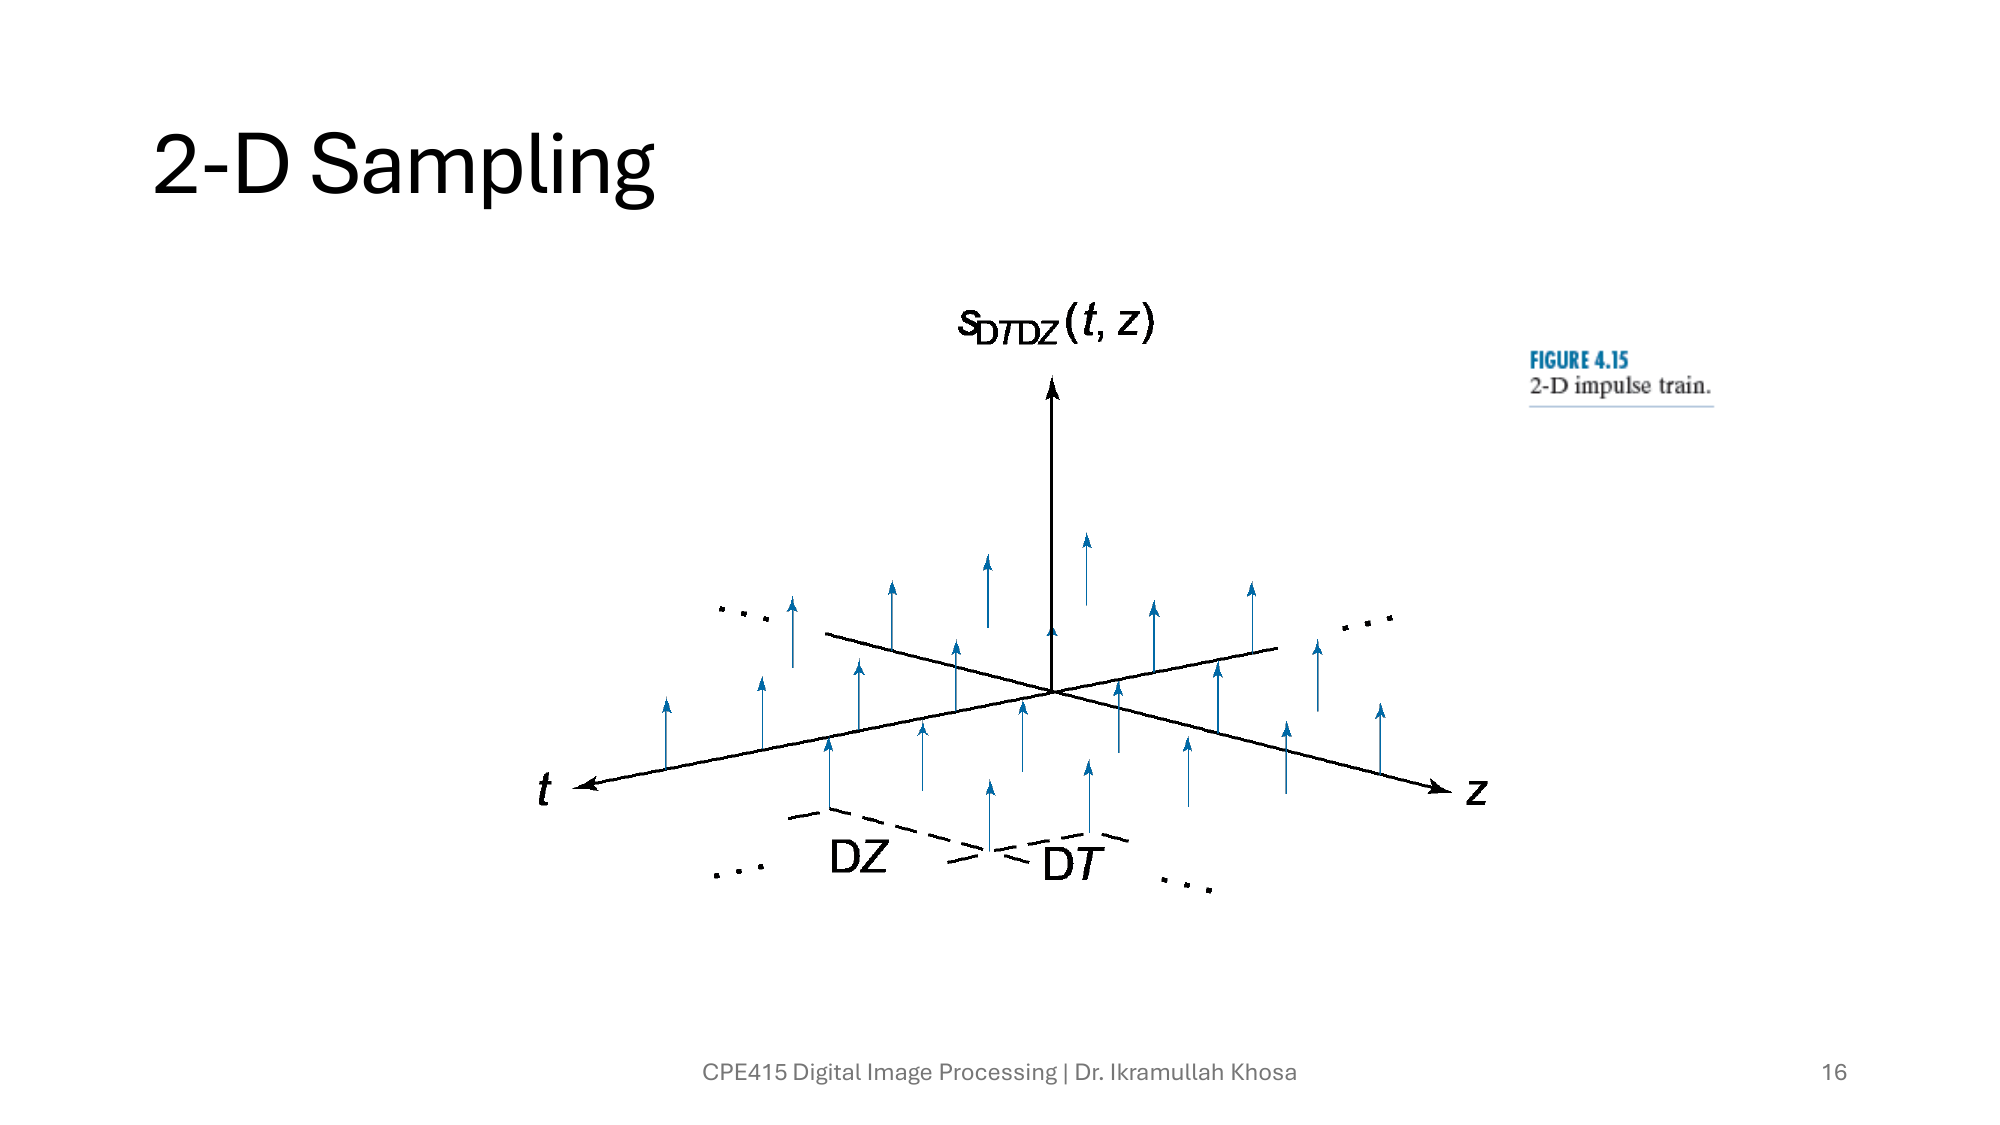
\includegraphics[width=0.85\textwidth]{images/slide8-16.png}
    \caption{2D sampling using a 2D impulse array}
    \label{fig:2d_sampling}
\end{figure}

\begin{deepexplanation}
\textbf{DEEP ANALYSIS - Figure \ref{fig:2d_sampling}: How Digital Images Are Formed}

\textbf{The 2D Impulse Array:}
\[
s(x, y) = \sum_{m=-\infty}^{\infty} \sum_{n=-\infty}^{\infty} \delta(x - m\Delta x, y - n\Delta y)
\]
where $\Delta x$ and $\Delta y$ are the horizontal and vertical pixel spacings.

\textbf{2D Sampling Operation:}
\[
\tilde{f}(x, y) = f(x, y) \cdot s(x, y)
\]

\textbf{What the Figure Illustrates:}
\begin{enumerate}
    \item \textbf{The continuous image} $f(x, y)$: Smooth, infinite resolution
    \item \textbf{The sampling grid}: Regular array of points (impulses)
    \item \textbf{The sampled image}: Values exist only at grid points
\end{enumerate}

\textbf{Physical Realization in Cameras:}
\begin{itemize}
    \item CCD/CMOS sensor = 2D array of photosites (``pixels'')
    \item Each photosite integrates light over its area (not a true impulse, but close)
    \item Pixel spacing determines spatial sampling frequency
    \item For a sensor with $N_x \times N_y$ pixels and dimensions $W \times H$: $\Delta x = W/N_x$, $\Delta y = H/N_y$
\end{itemize}

\textbf{Frequency Domain Effect:}
The Fourier transform of the 2D impulse array is another 2D impulse array:
\[
\mathcal{F}\{s(x, y)\} = \frac{1}{\Delta x \Delta y} \sum_{k} \sum_{l} \delta\left(u - \frac{k}{\Delta x}, v - \frac{l}{\Delta y}\right)
\]
This creates a 2D grid of spectral copies, leading to potential aliasing in both directions.
\end{deepexplanation}

\begin{figure}[H]
    \centering
    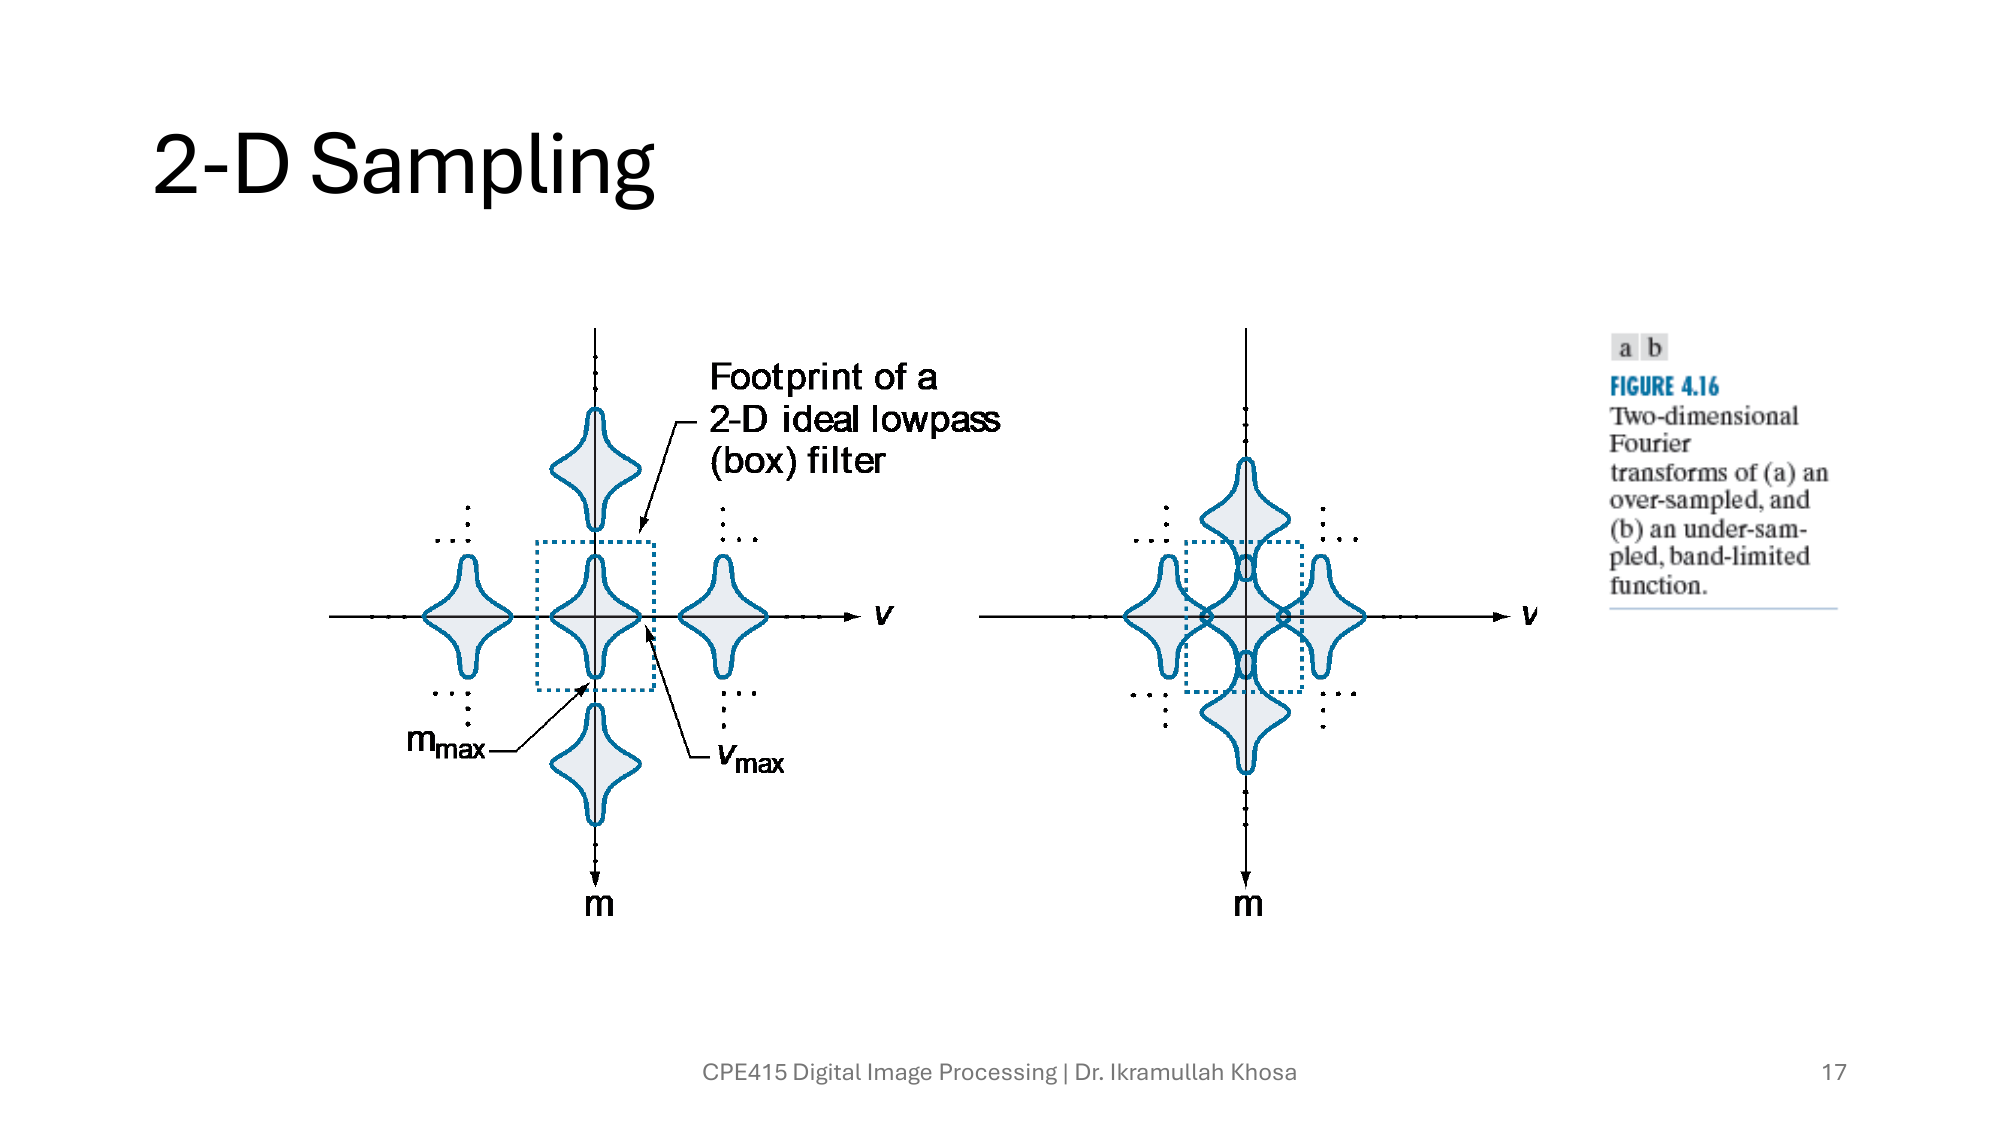
\includegraphics[width=0.85\textwidth]{images/slide8-17.png}
    \caption{2D sampling and spectral replication in frequency domain}
    \label{fig:2d_spectrum}
\end{figure}

\begin{deepexplanation}
\textbf{DEEP ANALYSIS - Figure \ref{fig:2d_spectrum}: 2D Spectral Copies and Potential Aliasing}

\textbf{The 2D Replication Pattern:}
After sampling, the spectrum becomes:
\[
\tilde{F}(u, v) = \frac{1}{\Delta x \Delta y} \sum_{k=-\infty}^{\infty} \sum_{l=-\infty}^{\infty} F\left(u - \frac{k}{\Delta x}, v - \frac{l}{\Delta y}\right)
\]

Copies of the original spectrum appear at every lattice point $(k/\Delta x, l/\Delta y)$.

\textbf{What the Figure Shows:}
\begin{itemize}
    \item Central spectrum (baseband) at origin
    \item 8 nearest neighbor copies (4 adjacent, 4 diagonal)
    \item Additional copies extending infinitely in both directions
    \item Spacing: $1/\Delta x$ horizontally, $1/\Delta y$ vertically
\end{itemize}

\textbf{2D Nyquist Condition:}
For no aliasing in 2D:
\[
\frac{1}{\Delta x} > 2 f_{x,max} \quad \text{and} \quad \frac{1}{\Delta y} > 2 f_{y,max}
\]
where $f_{x,max}$ and $f_{y,max}$ are the maximum spatial frequencies in the horizontal and vertical directions.

\textbf{The Diamond/Circular Problem:}
\begin{itemize}
    \item If the signal's spectrum is circular (radius $f_{max}$), diagonal frequencies can alias even when $x$ and $y$ directions satisfy Nyquist individually
    \item Maximum diagonal frequency: $\sqrt{f_{x,max}^2 + f_{y,max}^2}$
    \item Diagonal aliasing can occur at lower sampling rates than strictly horizontal/vertical aliasing
\end{itemize}
\end{deepexplanation}

%==============================================================================
\section{The Discrete Fourier Transform (DFT)}
%==============================================================================

\subsection{From Continuous to Discrete}

For digital processing, we need the Discrete Fourier Transform.

\begin{mathbox}
\textbf{2D Discrete Fourier Transform:}
\[
F(u, v) = \sum_{x=0}^{M-1} \sum_{y=0}^{N-1} f(x, y) e^{-j2\pi\left(\frac{ux}{M} + \frac{vy}{N}\right)}
\]
\textbf{Inverse DFT:}
\[
f(x, y) = \frac{1}{MN} \sum_{u=0}^{M-1} \sum_{v=0}^{N-1} F(u, v) e^{j2\pi\left(\frac{ux}{M} + \frac{vy}{N}\right)}
\]
\end{mathbox}

\begin{figure}[H]
    \centering
    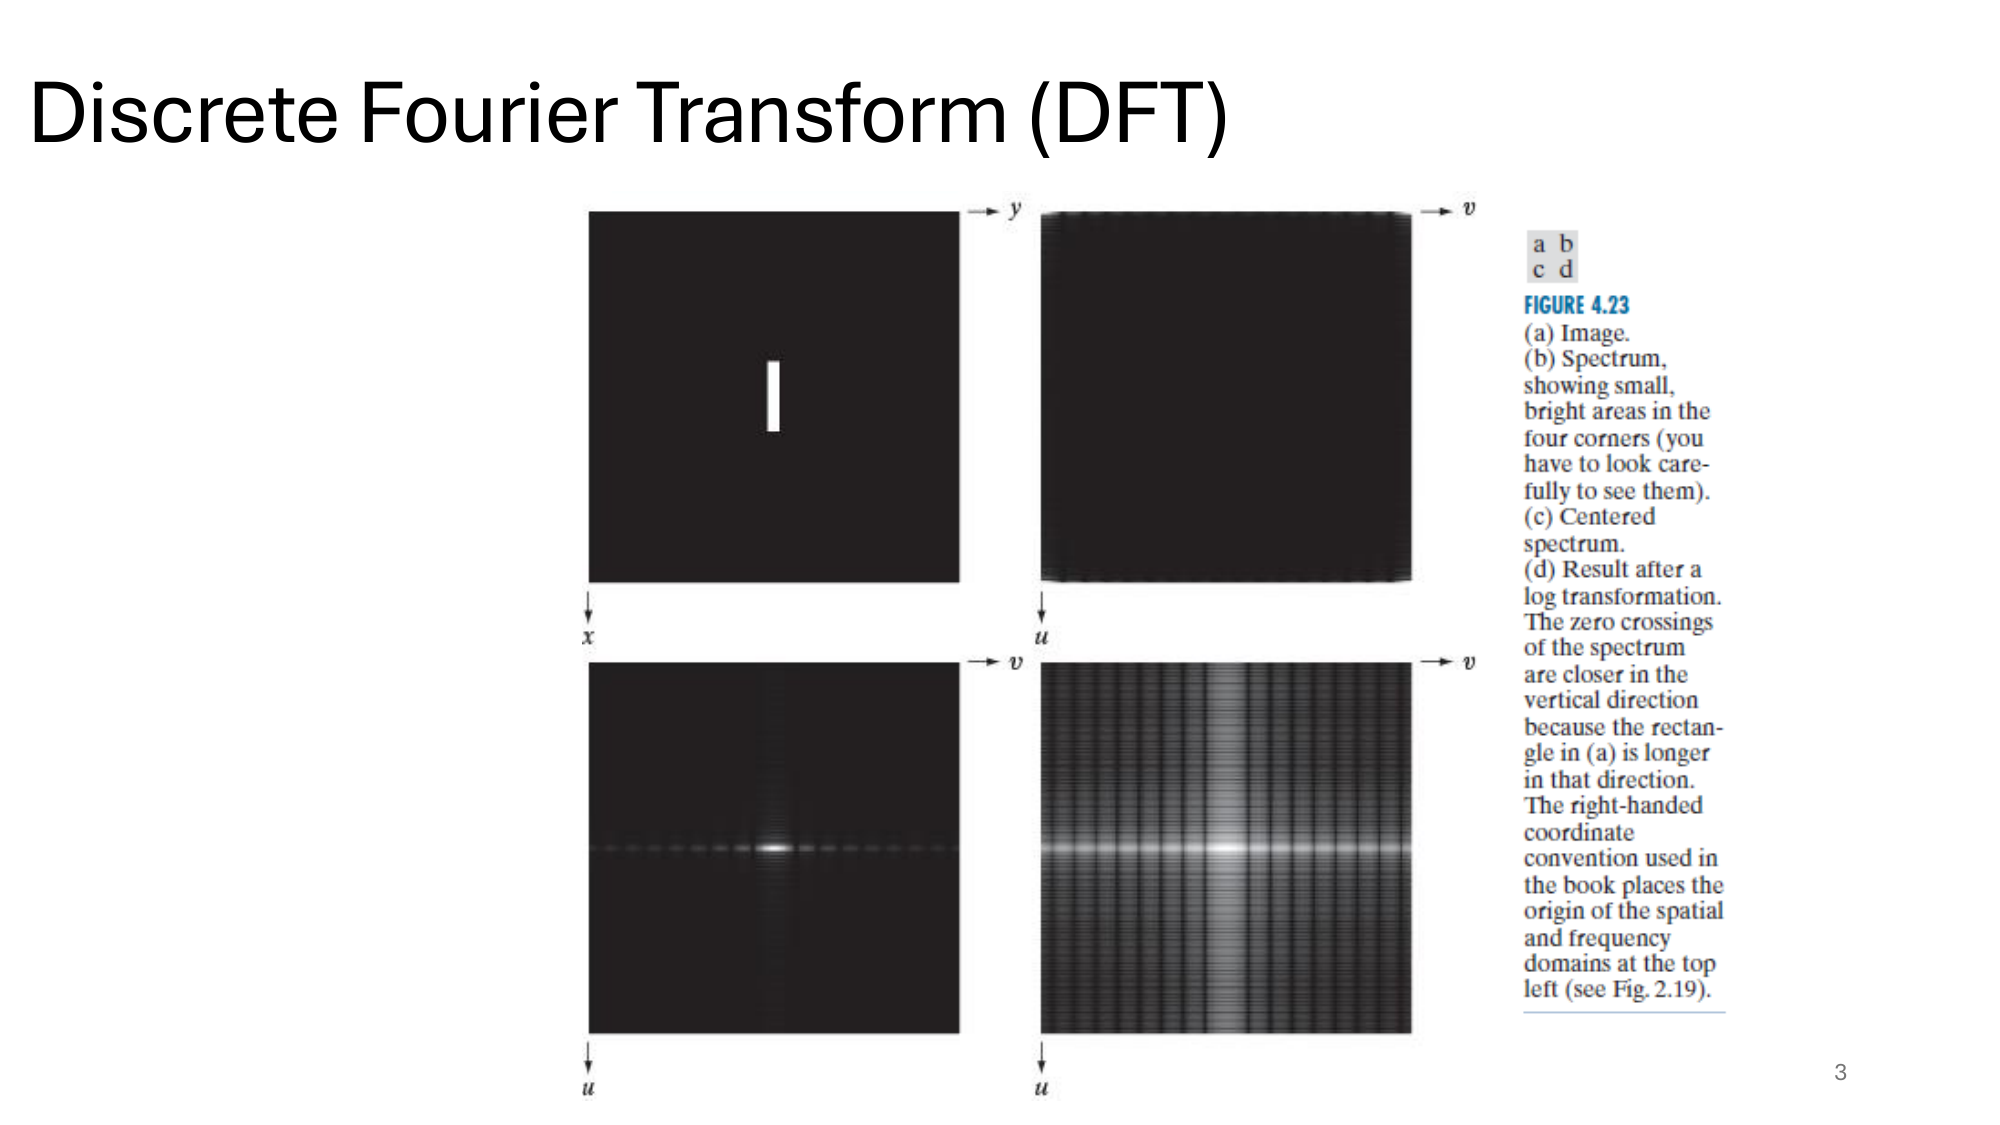
\includegraphics[width=0.9\textwidth]{images/slide9-03.png}
    \caption{DFT of a rectangle: (a) Image, (b) Spectrum, (c) Centered spectrum, (d) Log-transformed spectrum (FIGURE 4.23)}
    \label{fig:dft_computation}
\end{figure}

\begin{deepexplanation}
\textbf{DEEP ANALYSIS - Figure \ref{fig:dft_computation}: Understanding DFT Display and Centering}

\textbf{What This Figure Shows:}
A step-by-step visualization of computing and displaying the DFT of a simple rectangle:
\begin{itemize}
    \item \textbf{(a) Original image}: A vertical white rectangle on black background
    \item \textbf{(b) Raw spectrum}: DFT output with DC at corners (hard to interpret)
    \item \textbf{(c) Centered spectrum}: After applying ``fftshift'' --- DC now at center
    \item \textbf{(d) Log-transformed}: $\log(1 + |F|)$ for visibility of weak components
\end{itemize}

\textbf{Why Centering Is Essential:}
The raw DFT places the DC (zero frequency) at position $(0, 0)$, with high frequencies in the middle. This is mathematically correct but visually confusing. Centering rearranges so:
\begin{itemize}
    \item DC (average brightness) appears at center
    \item Low frequencies surround the center
    \item High frequencies are at edges/corners
    \item This matches our intuition about frequency
\end{itemize}

\textbf{Why Log Transform Is Necessary:}
\begin{itemize}
    \item The DC component is typically \textbf{much} larger than other frequencies
    \item Linear display: Only DC visible, everything else appears black
    \item Log compression: Reduces dynamic range, makes weak components visible
    \item Standard display: $D(u,v) = c \cdot \log(1 + |F(u,v)|)$
\end{itemize}

\textbf{Reading This Spectrum:}
\begin{itemize}
    \item The rectangle is taller than wide $\Rightarrow$ spectrum is wider than tall
    \item Sharp vertical edges $\Rightarrow$ strong horizontal line in spectrum
    \item Sinc-like ripples visible (Fourier transform of rect = sinc)
    \item Zero crossings correspond to $\sin(x)/x = 0$ at $x = n\pi$
\end{itemize}
\end{deepexplanation}

\subsection{Magnitude and Phase Spectra}

\begin{figure}[H]
    \centering
    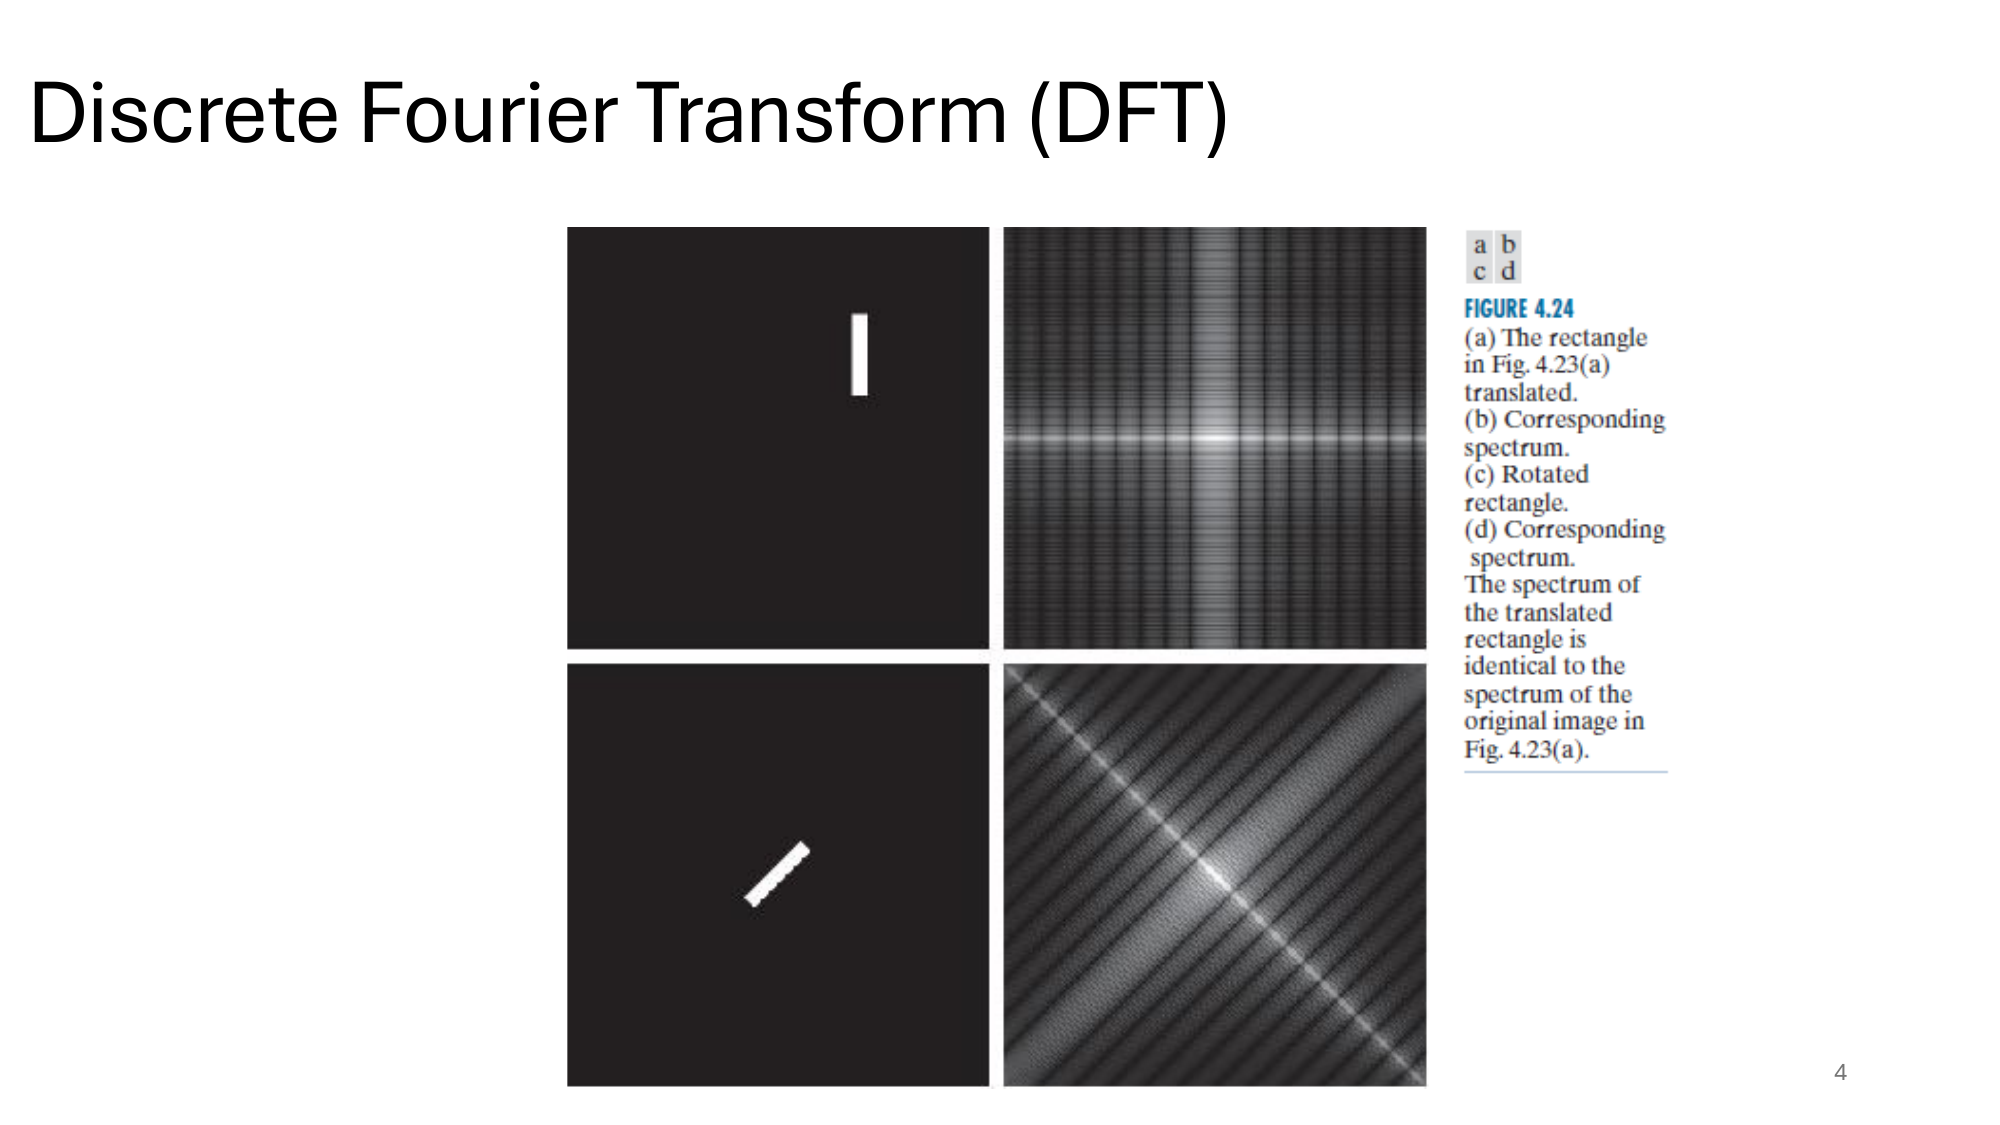
\includegraphics[width=0.9\textwidth]{images/slide9-04.png}
    \caption{Translation and rotation effects on spectrum (FIGURE 4.24)}
    \label{fig:image_spectrum}
\end{figure}

\begin{deepexplanation}
\textbf{DEEP ANALYSIS - Figure \ref{fig:image_spectrum}: How Translation and Rotation Affect the Spectrum}

\textbf{What This Figure Demonstrates:}
\begin{itemize}
    \item \textbf{(a)} Translated rectangle (moved from center)
    \item \textbf{(b)} Spectrum of translated rectangle --- \textbf{identical magnitude} to centered version!
    \item \textbf{(c)} Rotated rectangle (tilted 45°)
    \item \textbf{(d)} Spectrum of rotated rectangle --- \textbf{also rotated 45°}
\end{itemize}

\textbf{Key Fourier Transform Property \#1: Translation Invariance of Magnitude}
\[
f(x - x_0, y - y_0) \xrightarrow{\mathcal{F}} F(u, v) \cdot e^{-j2\pi(ux_0 + vy_0)}
\]
\begin{itemize}
    \item Translation in space $\Rightarrow$ Phase shift in frequency domain
    \item \textbf{Magnitude spectrum is unchanged!}
    \item This is why the spectrum of (a) looks identical to the centered rectangle's spectrum
    \item Position information is encoded entirely in phase
\end{itemize}

\textbf{Key Fourier Transform Property \#2: Rotation}
\[
f(x\cos\theta + y\sin\theta, -x\sin\theta + y\cos\theta) \xrightarrow{\mathcal{F}} F(u\cos\theta + v\sin\theta, -u\sin\theta + v\cos\theta)
\]
\begin{itemize}
    \item Rotation in space $\Rightarrow$ Same rotation in frequency domain
    \item The spectrum rotates by the same angle as the image
    \item Notice in (d): the sinc pattern is now oriented diagonally
\end{itemize}

\textbf{Practical Applications:}
\begin{itemize}
    \item \textbf{Pattern recognition}: Magnitude spectrum is translation-invariant, useful for detecting objects regardless of position
    \item \textbf{Rotation detection}: Compare spectrum orientations to find image rotation angle
    \item \textbf{Image registration}: Use these properties to align images
\end{itemize}
\end{deepexplanation}

\begin{figure}[H]
    \centering
    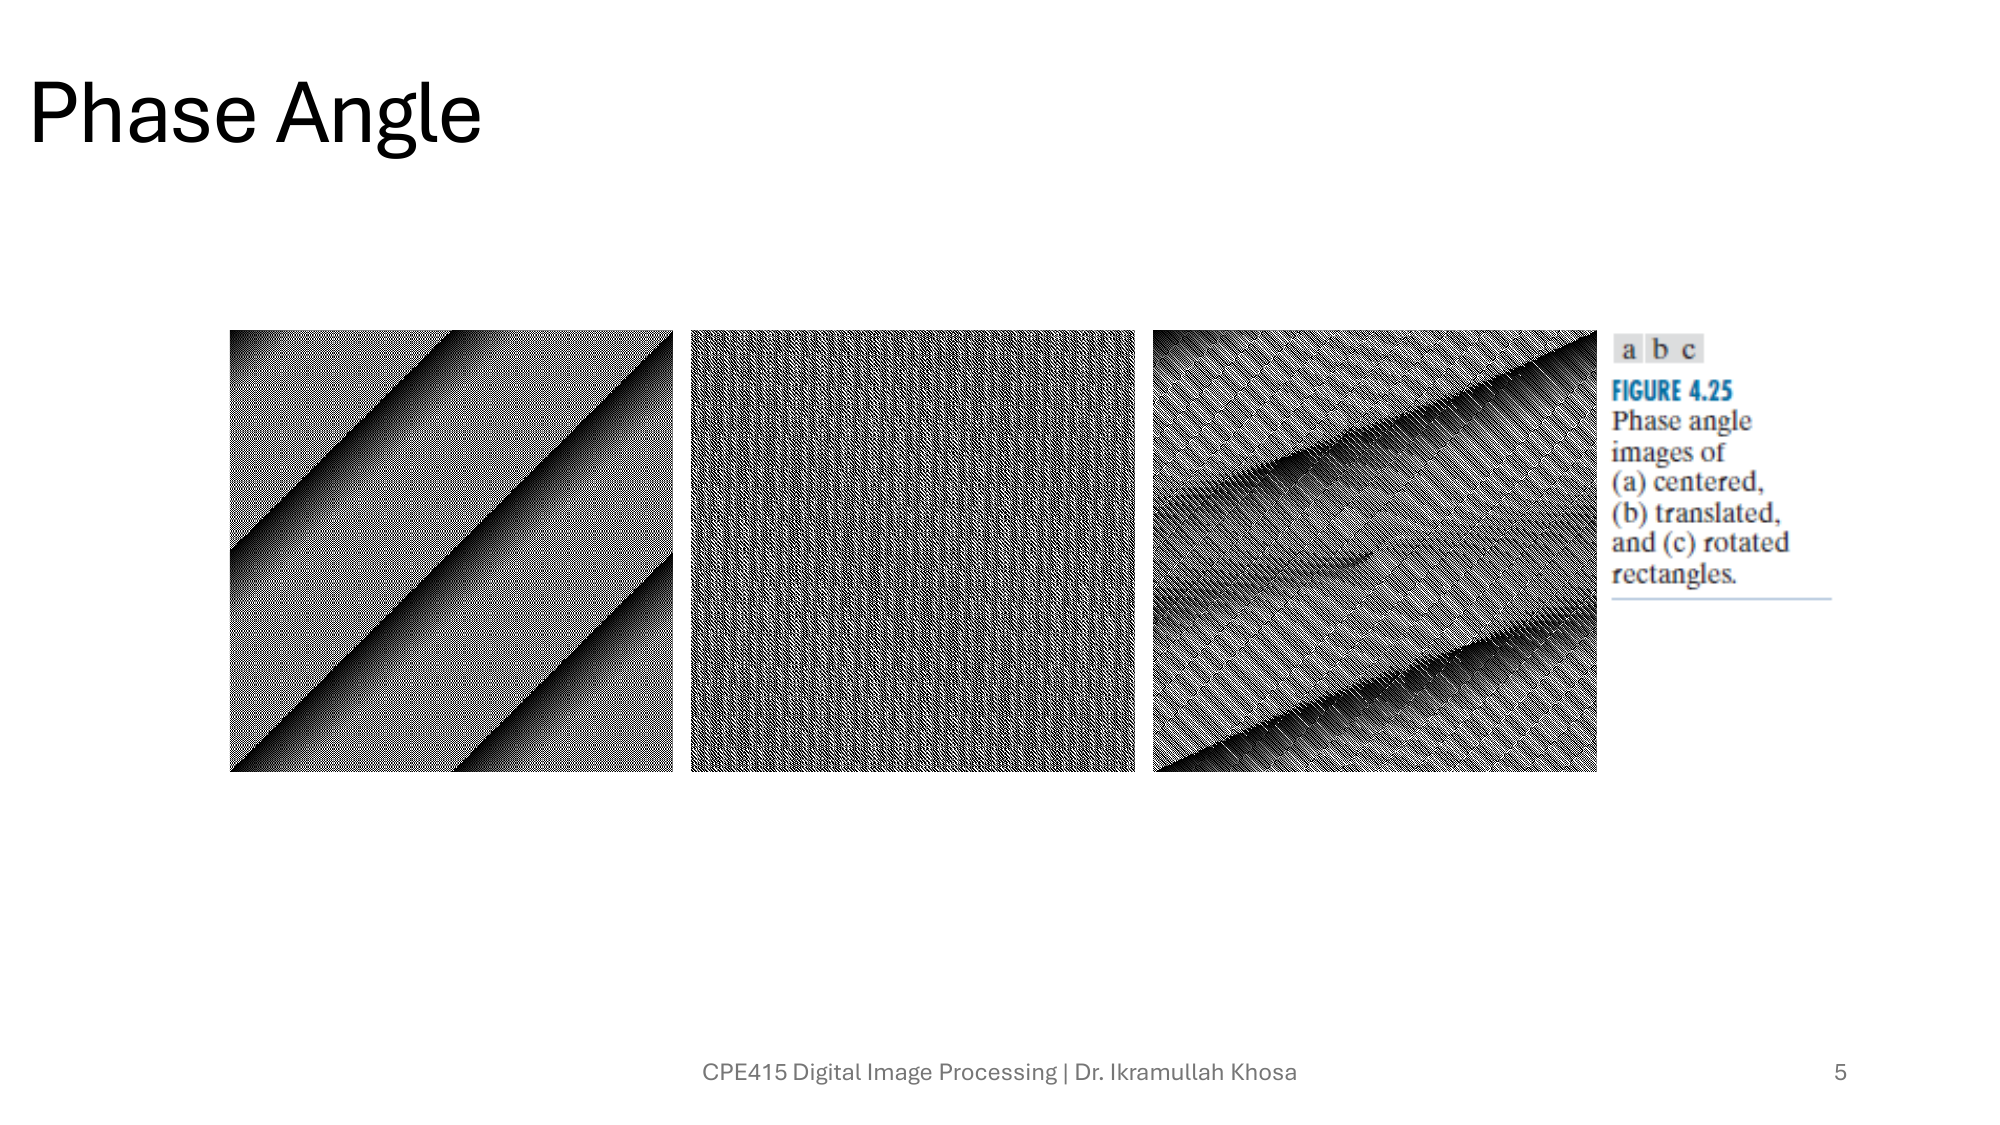
\includegraphics[width=0.85\textwidth]{images/slide9-05.png}
    \caption{Phase angle images of (a) centered, (b) translated, and (c) rotated rectangles (FIGURE 4.25)}
    \label{fig:phase_spectrum}
\end{figure}

\begin{deepexplanation}
\textbf{DEEP ANALYSIS - Figure \ref{fig:phase_spectrum}: How Phase Encodes Position and Orientation}

\textbf{What This Figure Shows:}
Phase angle spectra (displayed as grayscale images) for three rectangles:
\begin{itemize}
    \item \textbf{(a)} Centered rectangle: Smooth, symmetric phase pattern
    \item \textbf{(b)} Translated rectangle: Dramatically different phase pattern!
    \item \textbf{(c)} Rotated rectangle: Phase pattern also rotated
\end{itemize}

\textbf{Key Insight: Translation $\Leftrightarrow$ Linear Phase Shift}
\[
f(x - x_0, y - y_0) \xrightarrow{\mathcal{F}} F(u, v) \cdot e^{-j2\pi(ux_0/M + vy_0/N)}
\]
\begin{itemize}
    \item The exponential factor is a \textbf{linear phase ramp}
    \item Phase at each $(u, v)$ shifts by $-2\pi(ux_0/M + vy_0/N)$
    \item This creates the striped/ramp pattern visible in (b)
    \item The slope of the phase ramp encodes the translation amount
\end{itemize}

\textbf{Why Magnitude Is Unchanged But Phase Differs:}
\begin{itemize}
    \item Multiplying by $e^{j\theta}$ changes phase by $\theta$ but keeps magnitude constant
    \item All position information is in the phase!
    \item This is why phase is critical for accurate image reconstruction
\end{itemize}

\textbf{Phase Definition:}
\[
\phi(u, v) = \arctan\left(\frac{\text{Im}(F(u, v))}{\text{Re}(F(u, v))}\right)
\]

\textbf{Why Phase Matters More Than Magnitude:}
\begin{itemize}
    \item Phase encodes ``where'' each frequency component appears
    \item Sharp edges require precise phase alignment across frequencies
    \item Magnitude tells ``how much'' of each frequency exists
    \item Experiments show: Phase A + Magnitude B looks like Image A!
\end{itemize}
\end{deepexplanation}

\subsection{Image Reconstruction from Phase and Magnitude}

\begin{figure}[H]
    \centering
    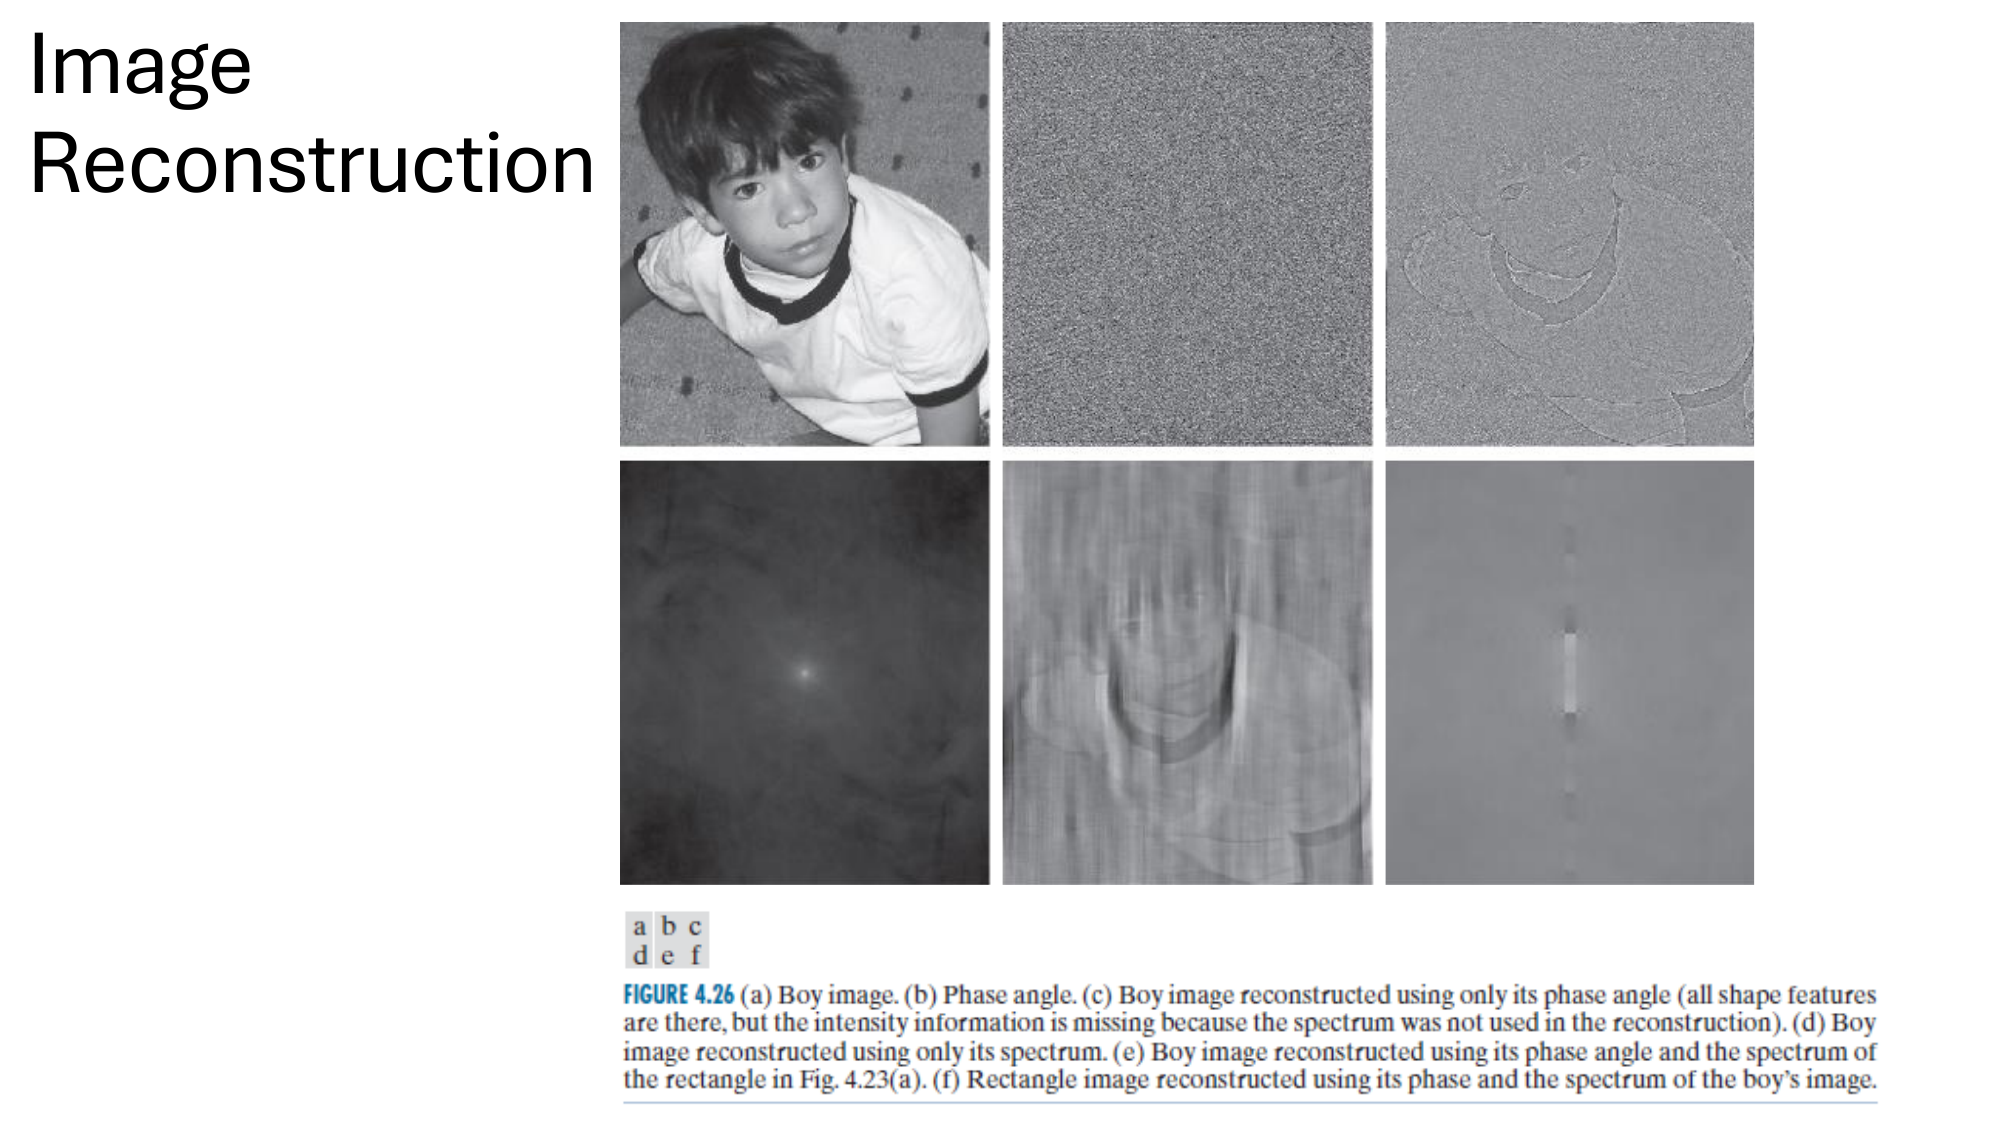
\includegraphics[width=0.9\textwidth]{images/slide9-06.png}
    \caption{FIGURE 4.26: Image reconstruction using phase and magnitude components separately}
    \label{fig:image_reconstruction}
\end{figure}

\begin{deepexplanation}
\textbf{DEEP ANALYSIS - Figure \ref{fig:image_reconstruction}: The Crucial Role of Phase vs Magnitude}

This figure demonstrates one of the most important insights in frequency domain analysis: \textbf{phase carries more structural information than magnitude}.

\textbf{What Each Panel Shows:}
\begin{itemize}
    \item \textbf{(a) Original boy image}: The input photograph used for this experiment
    \item \textbf{(b) Phase angle}: The phase spectrum $\phi(u,v) = \arctan\left(\frac{\text{Im}[F]}{\text{Re}[F]}\right)$ displayed as an image
    \item \textbf{(c) Reconstruction from phase only}: Image rebuilt using only phase information with uniform magnitude---all shape features are preserved but intensity is wrong
    \item \textbf{(d) Reconstruction from magnitude only}: Image rebuilt using only magnitude $|F(u,v)|$ with zero phase---appears as noise with no recognizable structure
    \item \textbf{(e) Boy phase + rectangle magnitude}: Combining boy's phase with a different image's magnitude still produces recognizable boy
    \item \textbf{(f) Rectangle phase + boy magnitude}: The rectangle shape dominates even with boy's magnitude
\end{itemize}

\textbf{The Deep Insight:}
\begin{itemize}
    \item \textbf{Phase encodes WHERE}: Edge locations, object boundaries, spatial relationships
    \item \textbf{Magnitude encodes HOW MUCH}: Energy at each frequency, overall contrast
    \item Human visual perception relies heavily on edges and structure (phase) rather than absolute intensities (magnitude)
\end{itemize}

\textbf{Mathematical Understanding:}
The inverse DFT reconstructs $f(x,y)$ from $F(u,v) = |F(u,v)|e^{j\phi(u,v)}$. When phase is preserved but magnitude is uniform, the relative positions of frequency components are maintained, preserving edges. When only magnitude is kept (phase=0), all components add constructively at the origin, destroying spatial structure.

\textbf{Practical Implications:}
\begin{itemize}
    \item Phase corruption (e.g., from quantization) causes severe image degradation
    \item Watermarking and steganography often exploit the robustness of phase
    \item Image compression should preserve phase information carefully
\end{itemize}
\end{deepexplanation}

%==============================================================================
\section{Frequency Domain Filtering Framework}
%==============================================================================

\subsection{The General Filtering Process}

The steps for frequency domain filtering are:

\begin{enumerate}
    \item Pad the image to avoid wraparound (to size $2M \times 2N$)
    \item Multiply by $(-1)^{x+y}$ to center the spectrum
    \item Compute the DFT: $F(u, v) = \mathcal{F}\{f(x, y)\}$
    \item Multiply by filter: $G(u, v) = F(u, v) \cdot H(u, v)$
    \item Compute inverse DFT: $g(x, y) = \mathcal{F}^{-1}\{G(u, v)\}$
    \item Multiply by $(-1)^{x+y}$ to undo centering
    \item Extract the real part and crop to original size
\end{enumerate}

\begin{figure}[H]
    \centering
    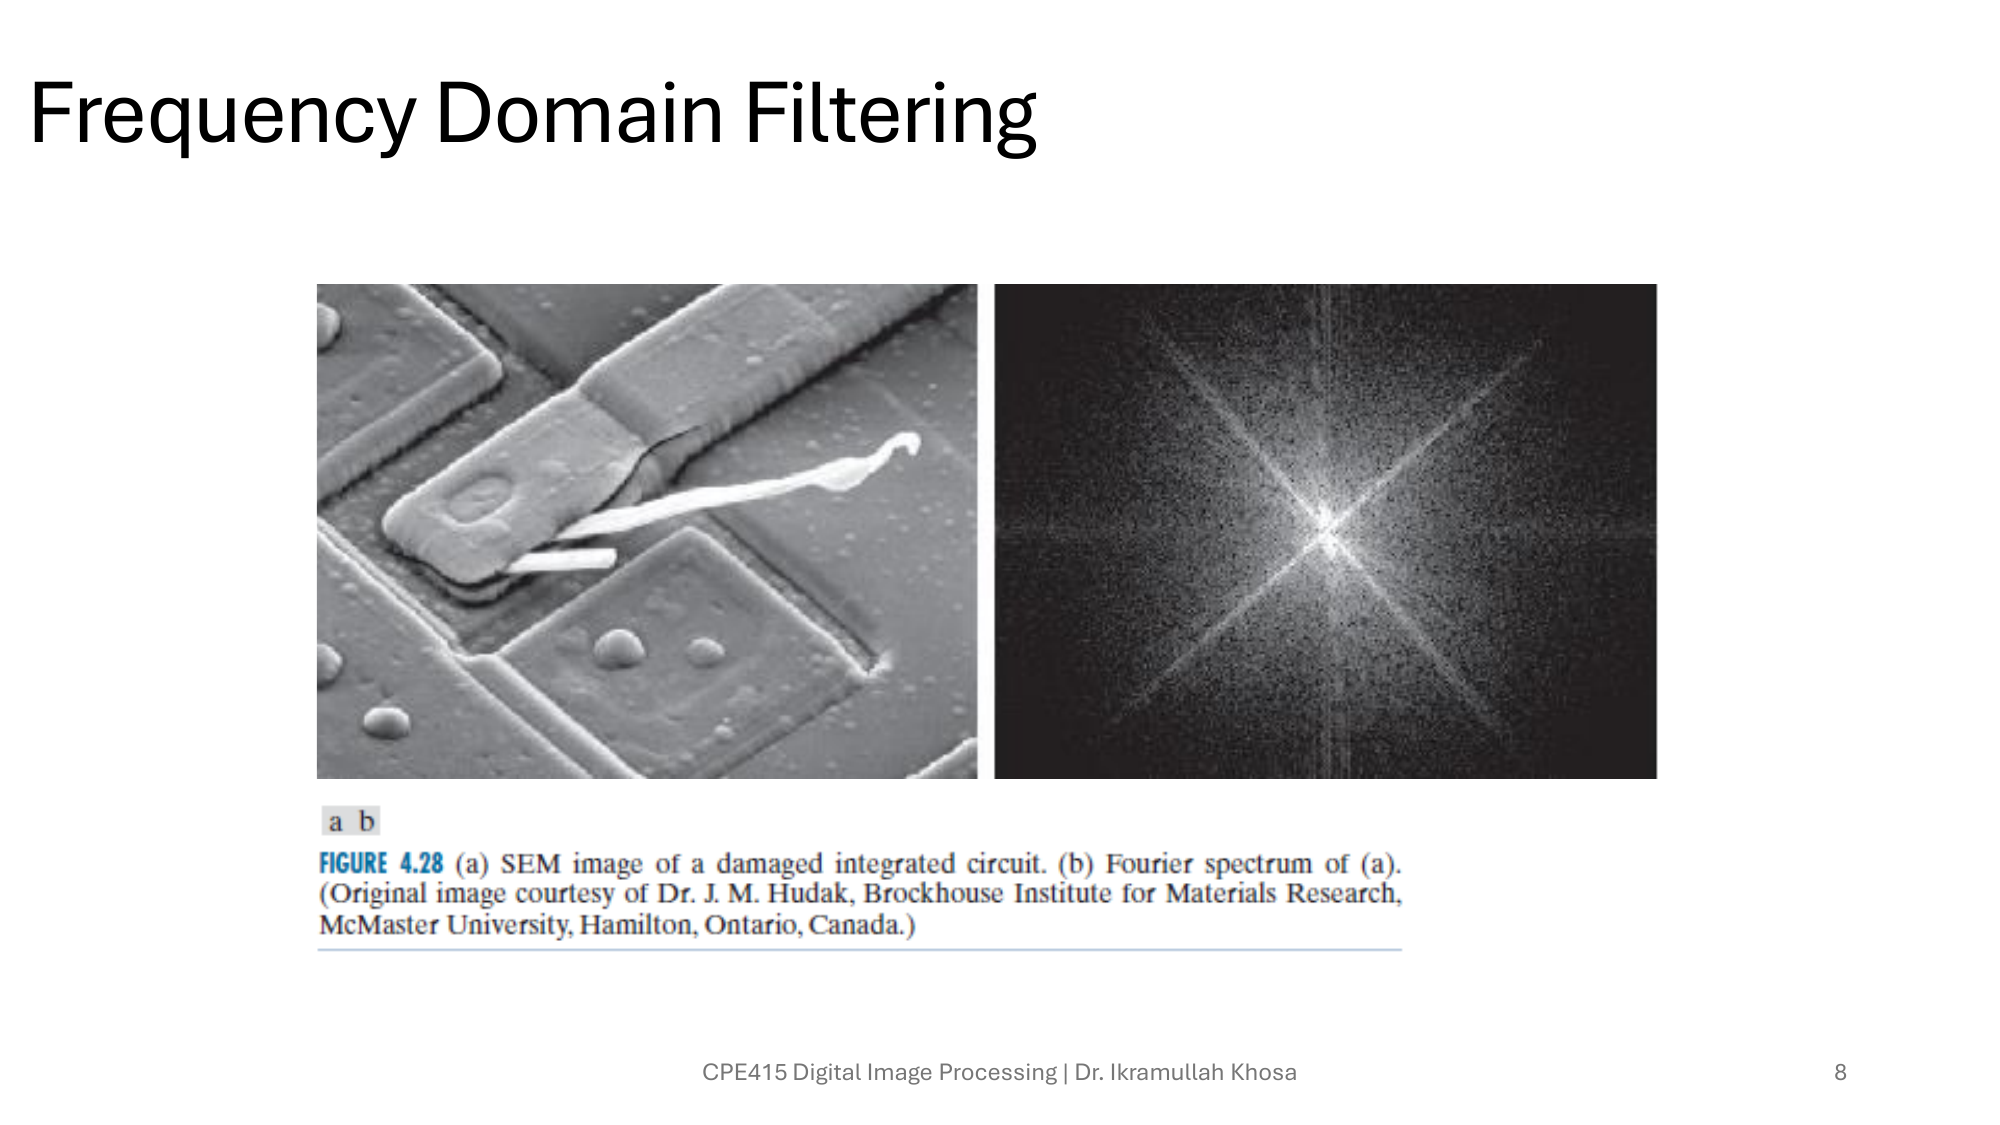
\includegraphics[width=0.95\textwidth]{images/slide9-08.png}
    \caption{FIGURE 4.28: (a) SEM image of a damaged integrated circuit. (b) Fourier spectrum of (a)}
    \label{fig:sem_spectrum}
\end{figure}

\begin{deepexplanation}
\textbf{DEEP ANALYSIS - Figure \ref{fig:sem_spectrum}: Understanding Image Spectra Through Real Examples}

This figure introduces frequency domain filtering using a compelling real-world example: a Scanning Electron Microscope (SEM) image of a damaged integrated circuit.

\textbf{What Panel (a) Shows - The SEM Image:}
\begin{itemize}
    \item A damaged integrated circuit with visible bond wires (the curved metallic connections)
    \item Sharp edges from the IC package and circuit traces
    \item Various textures: smooth metal surfaces, granular damage areas
    \item This complex image contains a rich mixture of frequencies
\end{itemize}

\textbf{What Panel (b) Shows - The Fourier Spectrum:}
\begin{itemize}
    \item \textbf{Bright center}: The DC component (average brightness)
    \item \textbf{X-shaped pattern}: Caused by the predominantly horizontal and vertical edges in the IC
    \item \textbf{Diagonal streaks}: From the angled bond wires in the image
    \item \textbf{Spread of energy}: Indicates the image contains significant high-frequency content (fine details)
\end{itemize}

\textbf{Reading the Spectrum:}
\begin{itemize}
    \item Strong horizontal line in spectrum $\rightarrow$ vertical edges in image
    \item Strong vertical line in spectrum $\rightarrow$ horizontal edges in image
    \item The spectrum reveals the dominant orientations and spatial frequencies present
\end{itemize}

\textbf{Why This Example Matters:}
This image will be used throughout the filtering sections to demonstrate how different filters (lowpass, highpass, notch) affect real image content. The variety of features makes it ideal for showing filter effects.
\end{deepexplanation}

\textbf{The General Filtering Process Steps:}
\begin{enumerate}
    \item Pad the image to avoid wraparound (to size $2M \times 2N$)
    \item Multiply by $(-1)^{x+y}$ to center the spectrum
    \item Compute the DFT: $F(u, v) = \mathcal{F}\{f(x, y)\}$
    \item Multiply by filter: $G(u, v) = F(u, v) \cdot H(u, v)$
    \item Compute inverse DFT: $g(x, y) = \mathcal{F}^{-1}\{G(u, v)\}$
    \item Multiply by $(-1)^{x+y}$ to undo centering
    \item Extract the real part and crop to original size
\end{enumerate}

\begin{figure}[H]
    \centering
    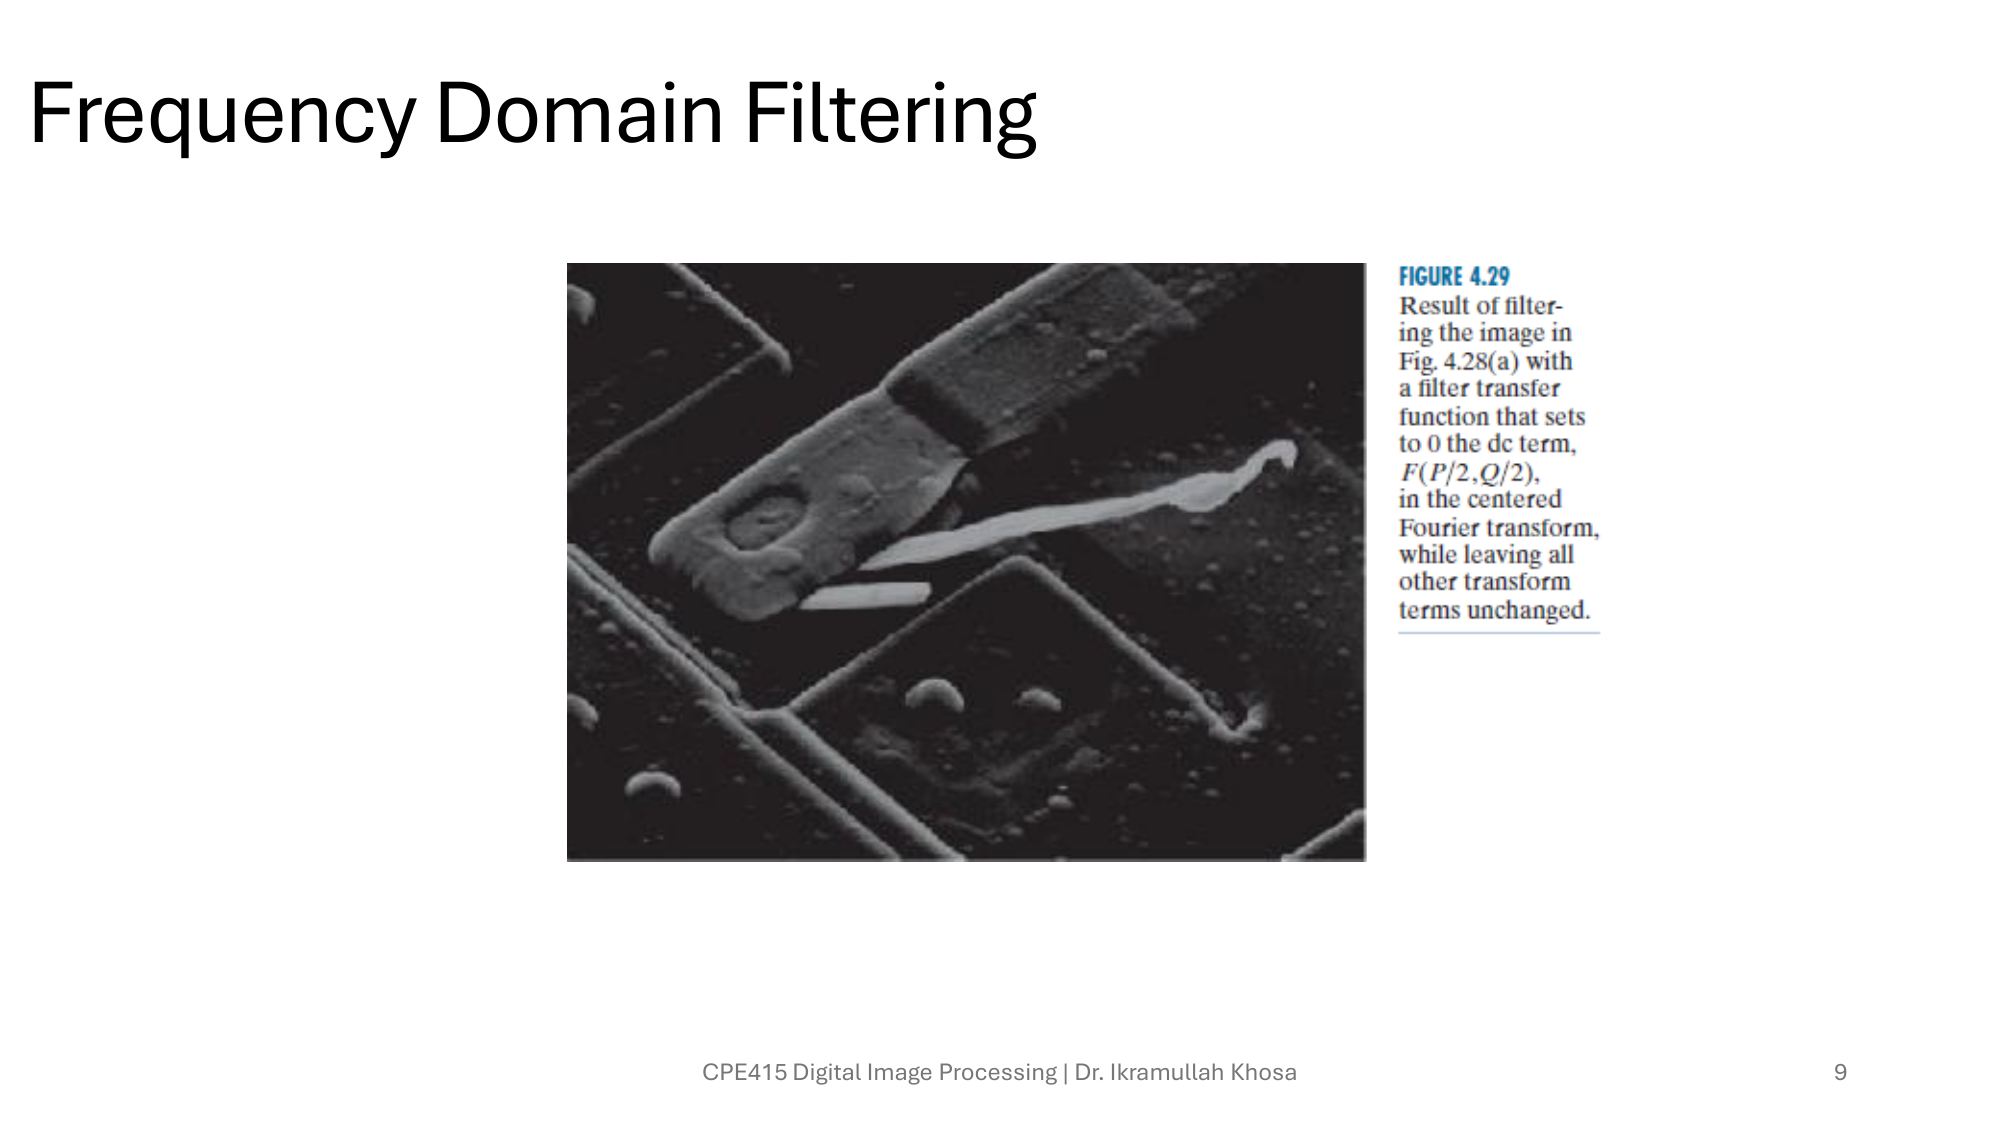
\includegraphics[width=0.9\textwidth]{images/slide9-09.png}
    \caption{FIGURE 4.29: Result of filtering the SEM image with a filter that sets the DC term to zero}
    \label{fig:dc_removal}
\end{figure}

\begin{deepexplanation}
\textbf{DEEP ANALYSIS - Figure \ref{fig:dc_removal}: DC Term Removal Demonstration}

This figure shows the simplest possible frequency domain filter: one that removes only the DC component while leaving all other frequencies unchanged.

\textbf{What the Figure Shows:}
The SEM image from Figure 4.28(a) after applying a filter $H(u,v)$ that satisfies:
\[
H(P/2, Q/2) = 0 \quad \text{and} \quad H(u,v) = 1 \text{ elsewhere}
\]
where $(P/2, Q/2)$ is the center of the centered Fourier transform.

\textbf{What Happens When DC Is Removed:}
\begin{itemize}
    \item The \textbf{average gray level} of the image becomes zero
    \item Originally bright areas appear as positive values (lighter than gray)
    \item Originally dark areas appear as negative values (darker than gray)
    \item After rescaling to $[0, 255]$, the image appears ``flatter'' with enhanced local contrast
\end{itemize}

\textbf{Mathematical Understanding:}
The DC component $F(0,0)$ equals:
\[
F(0,0) = \sum_{x=0}^{M-1} \sum_{y=0}^{N-1} f(x,y) = MN \cdot \bar{f}
\]
where $\bar{f}$ is the average pixel value. Setting $F(0,0) = 0$ subtracts the mean from every pixel.

\textbf{Practical Effect:}
\begin{itemize}
    \item Similar to ``local contrast enhancement''
    \item Removes overall illumination bias
    \item Makes the image ``zero-mean''
    \item Useful as preprocessing for correlation-based matching
\end{itemize}

This simple example demonstrates how modifying even a single frequency component can have a visible effect on the entire image.
\end{deepexplanation}


%==============================================================================
\section{Lowpass Filters: Smoothing in Frequency Domain}
%==============================================================================

Lowpass filters attenuate high frequencies, resulting in image smoothing/blurring.

\subsection{Ideal Lowpass Filter}

\begin{mathbox}
\textbf{Ideal Lowpass Filter:}
\[
H(u, v) = \begin{cases} 1 & D(u, v) \leq D_0 \\ 0 & D(u, v) > D_0 \end{cases}
\]
where $D(u, v) = \sqrt{(u - M/2)^2 + (v - N/2)^2}$ is the distance from center, and $D_0$ is the cutoff frequency.
\end{mathbox}

\begin{figure}[H]
    \centering
    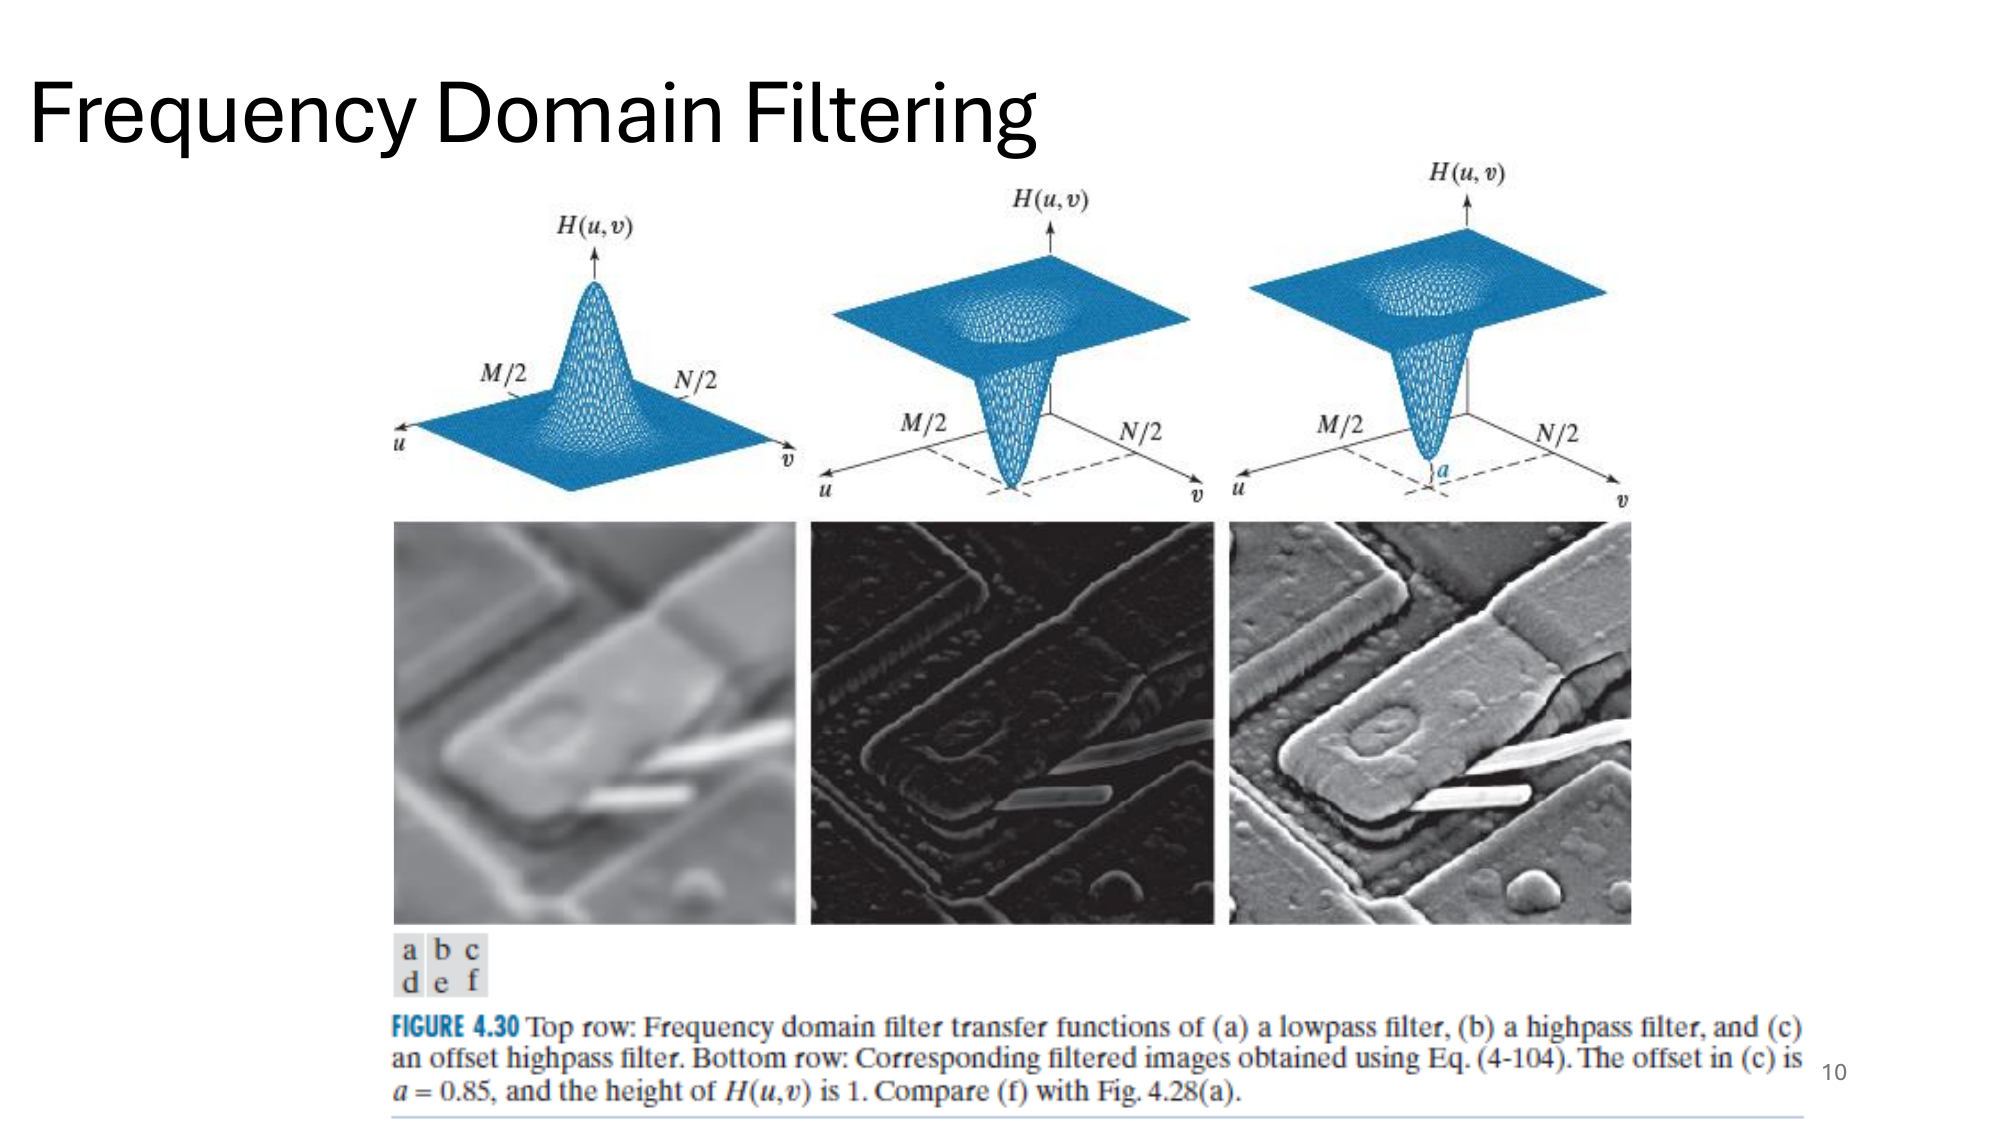
\includegraphics[width=0.85\textwidth]{images/slide9-10.png}
    \caption{FIGURE 4.30: Top row: Transfer functions of (a) lowpass, (b) highpass, and (c) offset highpass filters. Bottom row: Corresponding filtered images of the SEM IC}
    \label{fig:filter_comparison}
\end{figure}

\begin{deepexplanation}
\textbf{DEEP ANALYSIS - Figure \ref{fig:filter_comparison}: Comparing Three Fundamental Filter Types}

This crucial figure shows the three basic frequency domain filter types and their effects on a real image, providing visual intuition for filter design.

\textbf{Top Row - 3D Filter Transfer Functions $H(u,v)$:}

\textbf{(a) Lowpass Filter:}
\begin{itemize}
    \item \textbf{Shape}: Dome or bell-shaped, maximum at center (DC)
    \item \textbf{Behavior}: $H(u,v) = 1$ at center, decreases toward edges
    \item \textbf{Effect}: Passes low frequencies (smooth regions), blocks high frequencies (edges, noise)
\end{itemize}

\textbf{(b) Highpass Filter:}
\begin{itemize}
    \item \textbf{Shape}: Inverted dome, minimum (zero) at center
    \item \textbf{Behavior}: $H(u,v) = 0$ at center, increases toward edges
    \item \textbf{Effect}: Blocks DC and low frequencies, passes high frequencies (edges, details)
\end{itemize}

\textbf{(c) Offset (High-Frequency Emphasis) Filter:}
\begin{itemize}
    \item \textbf{Shape}: Similar to highpass but with raised baseline
    \item \textbf{Behavior}: $H(u,v) = a$ at center (where $0 < a < 1$), increases toward edges
    \item \textbf{Effect}: Preserves some DC (overall brightness) while emphasizing edges
    \item In this example, $a = 0.85$, meaning DC is attenuated to 85\%
\end{itemize}

\textbf{Bottom Row - Filtered Results on SEM Image:}

\textbf{(d) Lowpass Result:}
\begin{itemize}
    \item Image appears \textbf{blurred/smoothed}
    \item Fine details and noise are removed
    \item Overall structure preserved but edges softened
\end{itemize}

\textbf{(e) Highpass Result:}
\begin{itemize}
    \item Only \textbf{edges and fine details} remain
    \item Image appears mostly dark (DC removed)
    \item Shows where rapid intensity changes occur
\end{itemize}

\textbf{(f) Offset Highpass Result:}
\begin{itemize}
    \item \textbf{Sharpened appearance} with enhanced edges
    \item Retains overall brightness (compare with panel a)
    \item Best of both worlds: structure + enhanced details
    \item This is the basis for ``unsharp masking'' sharpening
\end{itemize}

\textbf{Key Insight:} The offset filter shows why highpass filtering alone produces unusable images (no DC = no overall brightness), and how adding back a fraction of low frequencies creates useful edge enhancement.
\end{deepexplanation}

\begin{figure}[H]
    \centering
    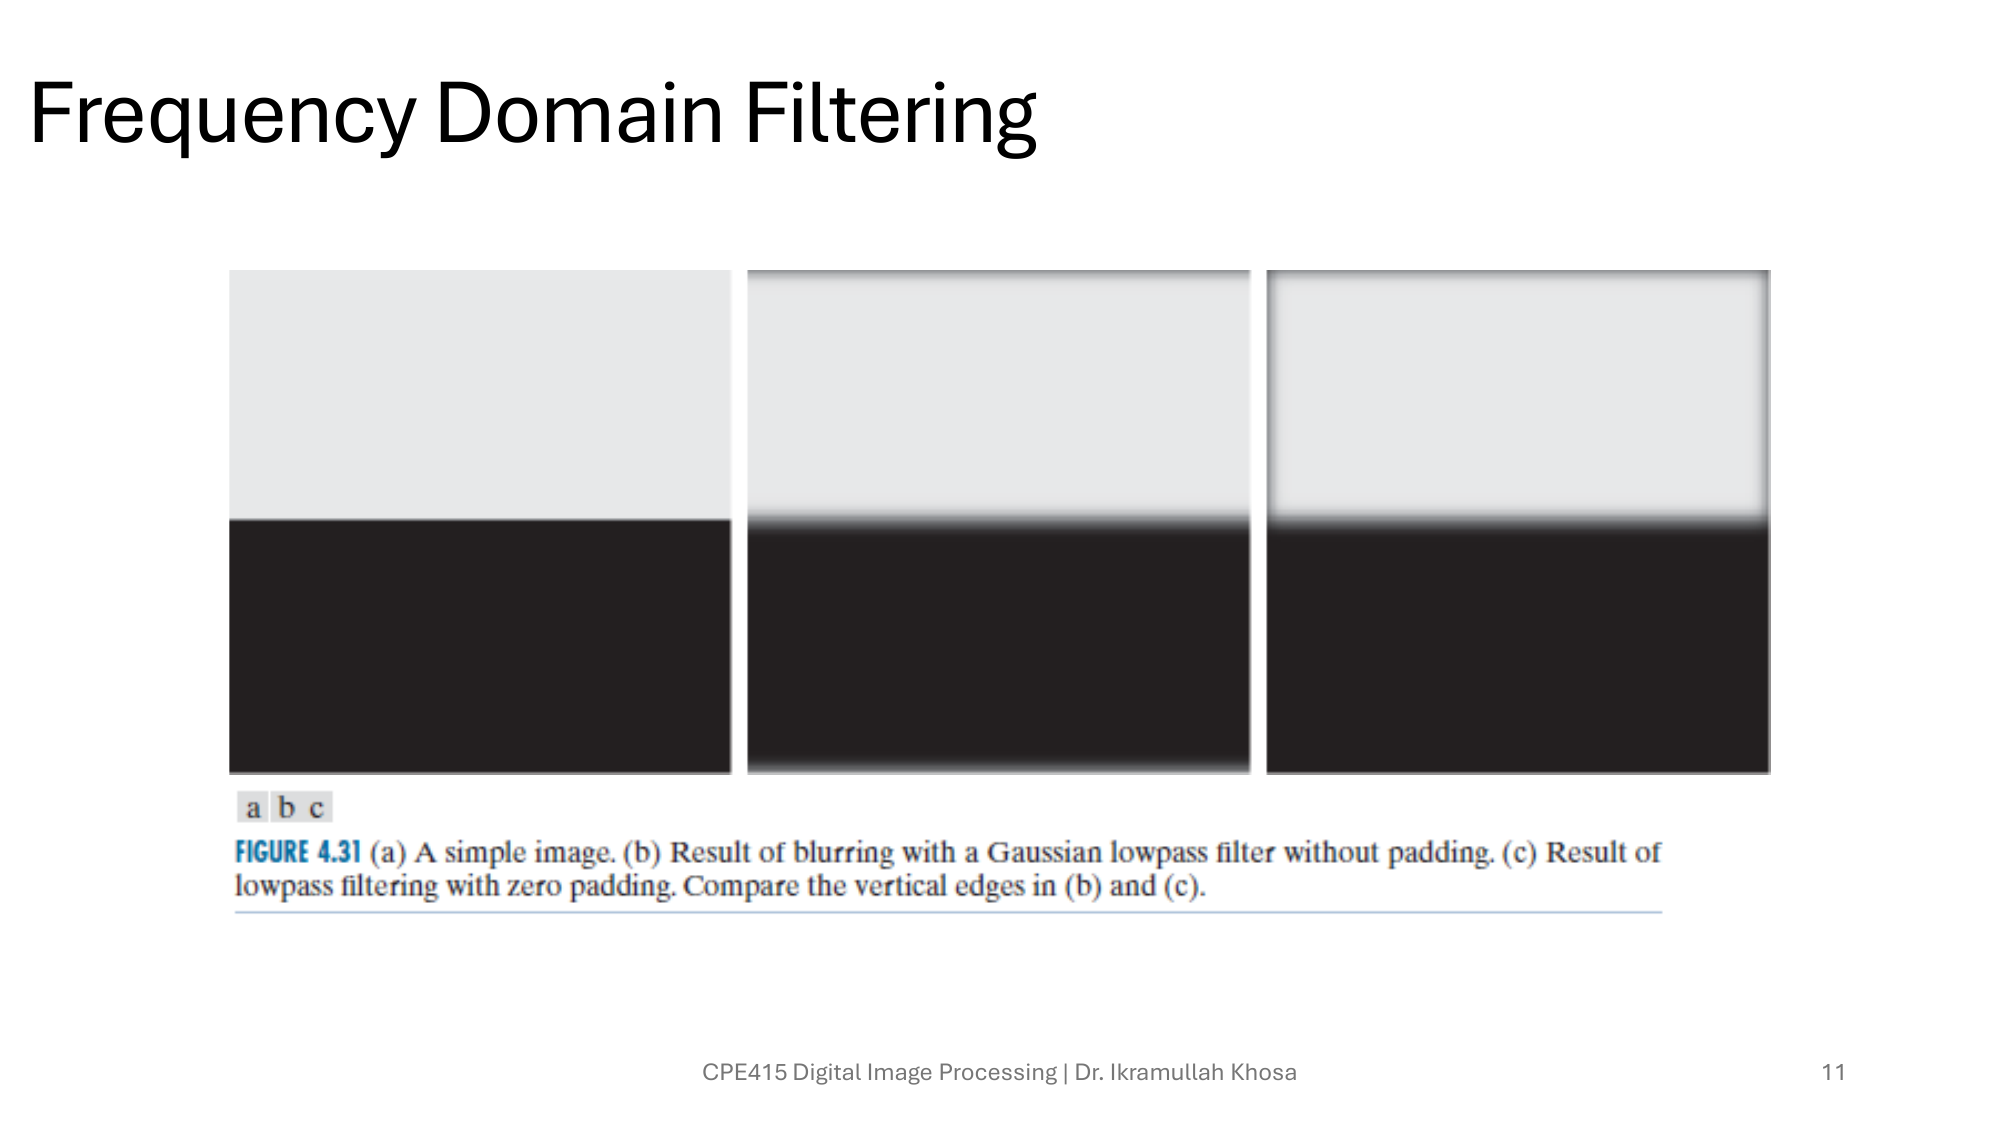
\includegraphics[width=0.95\textwidth]{images/slide9-11.png}
    \caption{FIGURE 4.31: (a) Simple test image. (b) Gaussian lowpass filtered without padding - note vertical edge artifacts. (c) Filtered with zero padding - clean edges}
    \label{fig:padding_effect}
\end{figure}

\begin{deepexplanation}
\textbf{DEEP ANALYSIS - Figure \ref{fig:padding_effect}: Why Zero Padding Is Essential}

This figure demonstrates a critical practical issue in frequency domain filtering: the wraparound error that occurs without proper padding.

\textbf{The Test Image (a):}
A simple image with a sharp horizontal edge---white on top, black on bottom. This simplicity makes wraparound artifacts clearly visible.

\textbf{What Happens Without Padding (b):}
\begin{itemize}
    \item The DFT treats the image as \textbf{infinitely periodic} (tiling in all directions)
    \item When the image tiles, black bottom touches white top, creating artificial edges
    \item The lowpass filter blurs these artificial edges
    \item The blur ``wraps around'' from one side to the other
    \item \textbf{Result}: Vertical gradients appear near the left and right edges where none should exist
\end{itemize}

\textbf{What Happens With Zero Padding (c):}
\begin{itemize}
    \item Image is padded to at least $2M \times 2N$ with zeros
    \item When padded image tiles, black regions (zeros) separate the image copies
    \item No artificial edges are created by tiling
    \item Filter effects don't wrap from one side to the other
    \item \textbf{Result}: Clean horizontal edge, no vertical artifacts
\end{itemize}

\textbf{The Math Behind It:}
\begin{itemize}
    \item Spatial convolution has output size $(M+m-1) \times (N+n-1)$ for $M \times N$ image and $m \times n$ kernel
    \item DFT-based convolution produces circular convolution of size $M \times N$
    \item To match linear convolution, pad to at least $(M+m-1) \times (N+n-1)$
    \item Since filter kernels can be large (especially for ideal filters), $2M \times 2N$ padding is standard
\end{itemize}

\textbf{Practical Rule:}
\textit{Always zero-pad before frequency domain filtering, then crop the result back to original size.}
\end{deepexplanation}

\begin{deepexplanation}
\textbf{DEEP ANALYSIS - Figure \ref{fig:ideal_lpf_effect}: Cutoff Frequency Impact}

\textbf{What the Figure Shows:}
A series of images filtered with ideal lowpass filters at different cutoff radii, typically:
\begin{itemize}
    \item Original image (unfiltered)
    \item $D_0$ = 5: Severe blur, only gross structure visible
    \item $D_0$ = 15: Moderate blur, main shapes preserved
    \item $D_0$ = 30: Slight blur, most details preserved
    \item $D_0$ = 80: Nearly original, finest details smoothed
\end{itemize}

\textbf{Quantitative Analysis:}

\textbf{Energy Enclosed:} For natural images with $1/f^2$ spectrum:
\begin{itemize}
    \item $D_0$ enclosing 85\% energy: Significant detail loss
    \item $D_0$ enclosing 95\% energy: Subtle smoothing
    \item $D_0$ enclosing 99\% energy: Barely perceptible effect
\end{itemize}

\textbf{Observing Ringing:}
\begin{itemize}
    \item Most visible at low $D_0$ values
    \item Look for ``halos'' around sharp edges
    \item Bright/dark bands parallel to strong edges
    \item More visible in high-contrast regions
\end{itemize}

\textbf{Practical Applications:}
\begin{itemize}
    \item Noise reduction (noise is often high-frequency)
    \item Scale-space analysis (progressive blurring)
    \item Image pyramid construction
    \item Pre-filtering before downsampling (anti-aliasing)
\end{itemize}
\end{deepexplanation}

\subsection{Understanding Image Periodicity and Wraparound}

\begin{figure}[H]
    \centering
    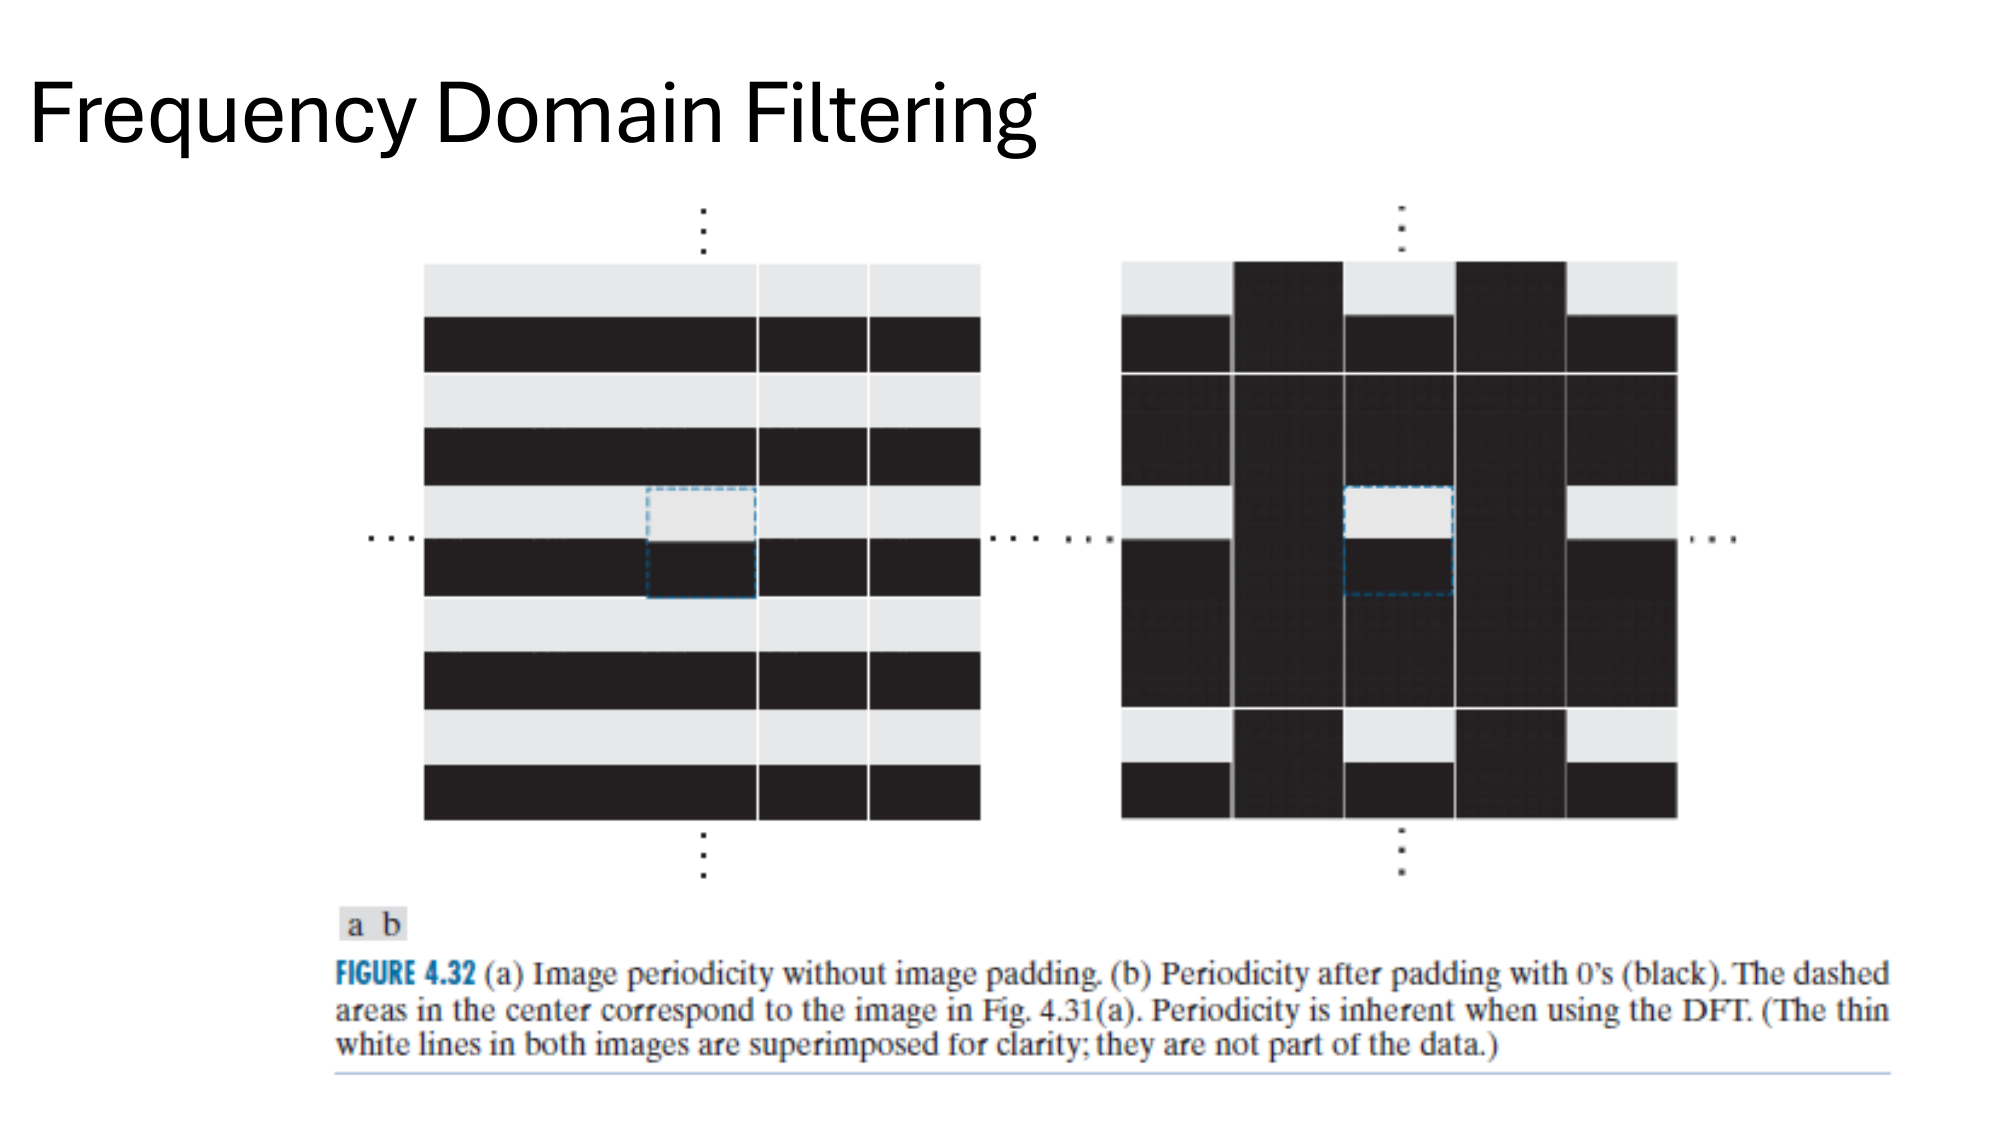
\includegraphics[width=0.85\textwidth]{images/slide9-12.png}
    \caption{FIGURE 4.32: (a) Image periodicity without padding - adjacent copies touch. (b) Periodicity after zero padding - copies separated by black buffer zones}
    \label{fig:periodicity}
\end{figure}

\begin{deepexplanation}
\textbf{DEEP ANALYSIS - Figure \ref{fig:periodicity}: Visualizing DFT's Implicit Periodicity}

This figure provides crucial insight into why zero padding is necessary for proper frequency domain filtering.

\textbf{The Fundamental Issue:}
The Discrete Fourier Transform (DFT) implicitly assumes the input signal is \textbf{one period of an infinitely periodic function}. When you compute the DFT of an image, the math ``sees'' infinite copies tiled in all directions.

\textbf{Panel (a) - Without Padding:}
\begin{itemize}
    \item Shows the simple test image (from FIGURE 4.31) tiled infinitely
    \item The dashed box marks the actual image region
    \item \textbf{Problem}: Black bottom of one copy directly touches white top of next copy
    \item This creates \textbf{artificial edges} that don't exist in the original image
    \item When convolution is performed via DFT multiplication, these artificial edges get blurred
    \item The blur ``wraps around'' to appear on the opposite side of the image
\end{itemize}

\textbf{Panel (b) - With Zero Padding:}
\begin{itemize}
    \item The image is padded with zeros (black) to double its size before DFT
    \item When this padded image tiles, black regions separate the copies
    \item \textbf{Solution}: No artificial edges between copies---only gradual transitions through zeros
    \item Convolution effects stay local; no wraparound artifacts
    \item After filtering, crop back to original size to get clean result
\end{itemize}

\textbf{Why 2× Padding?}
For an $M \times N$ image convolved with kernel up to $M \times N$:
\begin{itemize}
    \item Linear convolution output size: $(2M-1) \times (2N-1)$
    \item Padding to $2M \times 2N$ ensures sufficient room
    \item This is the minimum; more padding is occasionally used for finer frequency resolution
\end{itemize}

\textbf{Key Takeaway:}
\textit{The thin white lines are for visualization only. In practice, zero padding prevents the ``tiled copies'' from interfering with each other during frequency domain operations.}
\end{deepexplanation}

\subsection{Filter Design: Frequency vs Spatial Domain Relationship}

\begin{figure}[H]
    \centering
    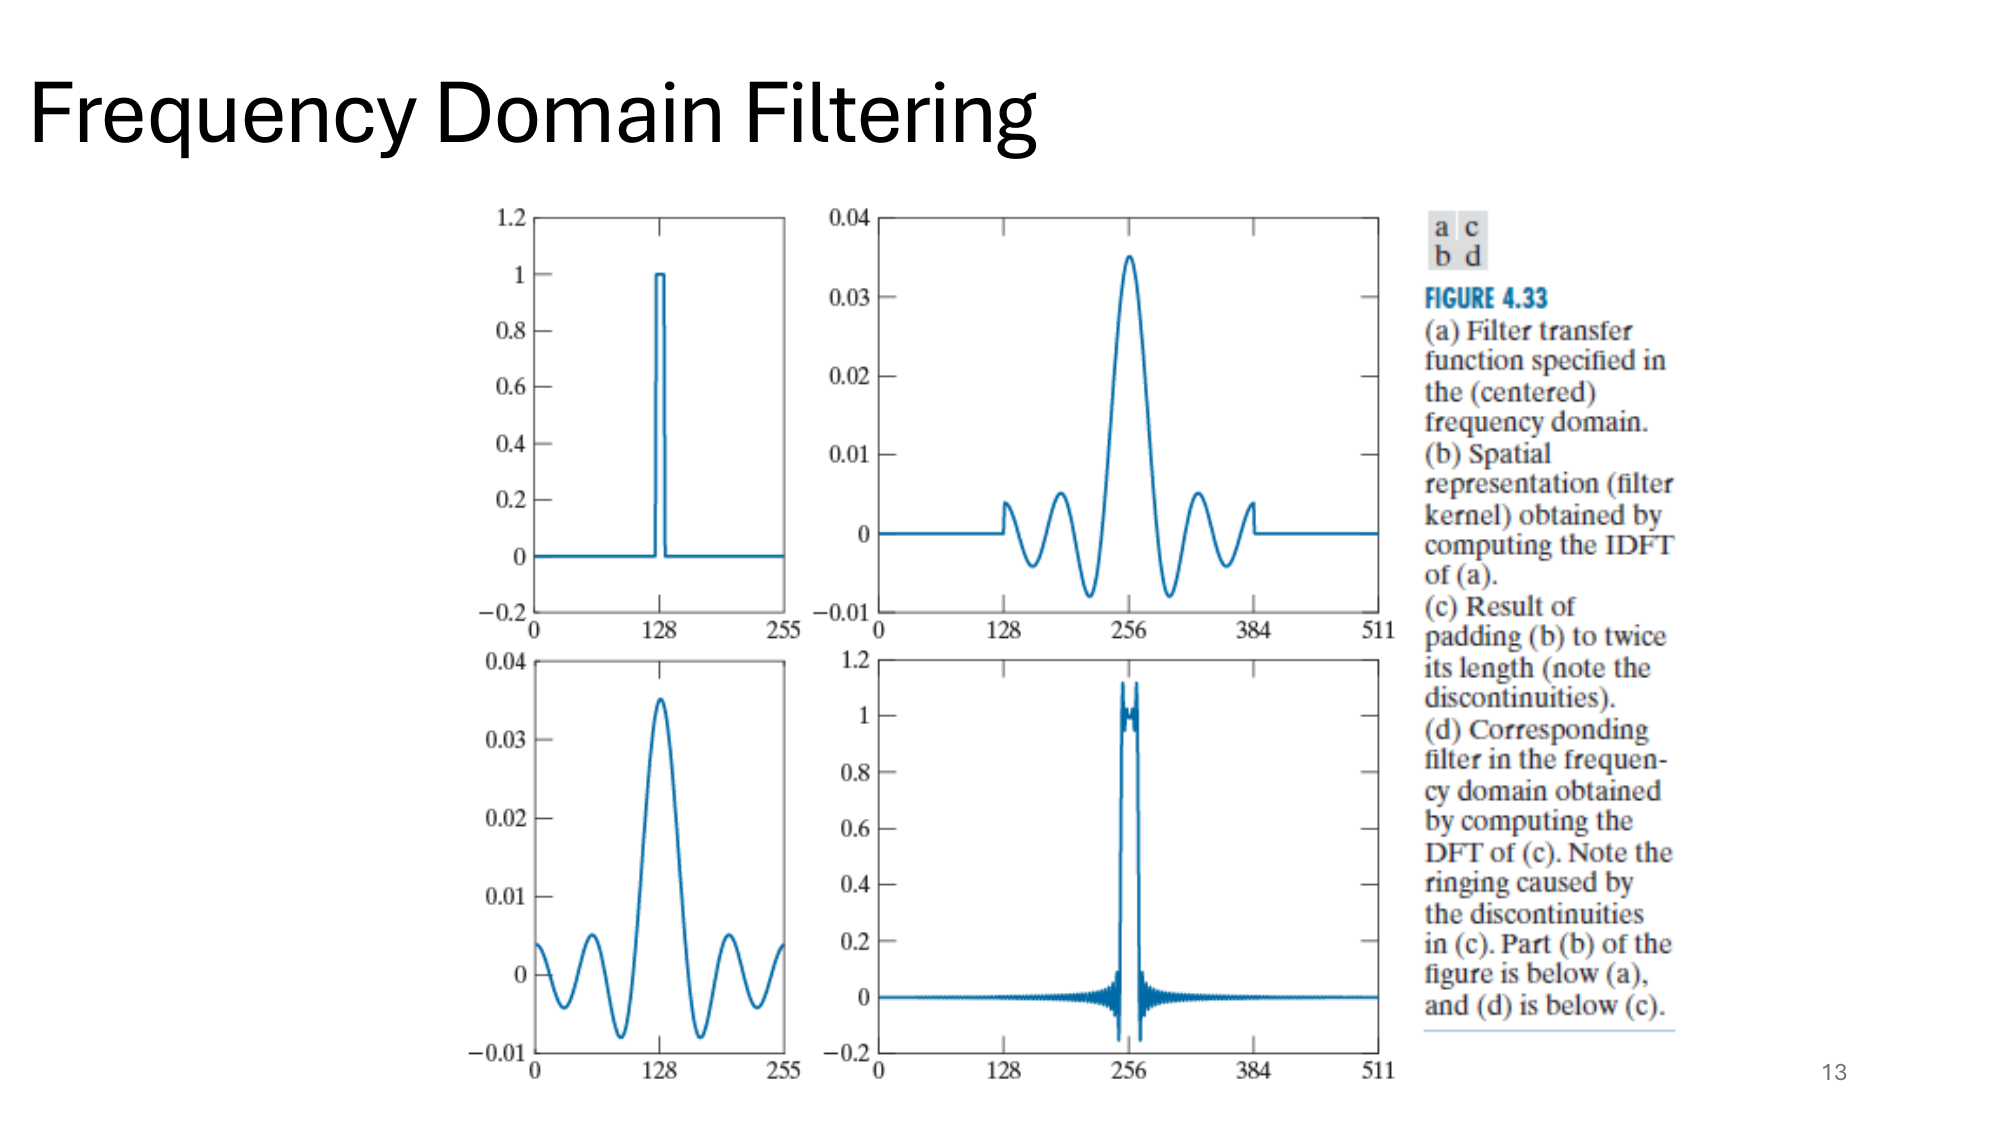
\includegraphics[width=0.95\textwidth]{images/slide9-13.png}
    \caption{FIGURE 4.33: Relationship between frequency domain filter and spatial domain kernel, showing effects of padding}
    \label{fig:filter_spatial_relationship}
\end{figure}

\begin{deepexplanation}
\textbf{DEEP ANALYSIS - Figure \ref{fig:filter_spatial_relationship}: Frequency and Spatial Domain Duality}

This figure illustrates a fundamental concept: every frequency domain filter has a corresponding spatial domain kernel, and padding affects both representations.

\textbf{Panel (a) - Frequency Domain Filter $H(u,v)$:}
\begin{itemize}
    \item A centered lowpass filter transfer function
    \item Smooth bell-shaped curve from 1.0 at center to 0 at edges
    \item This is how we typically \textit{design} frequency domain filters
\end{itemize}

\textbf{Panel (b) - Spatial Domain Kernel $h(x,y)$ via IDFT:}
\begin{itemize}
    \item Computing $\mathcal{F}^{-1}\{H(u,v)\}$ gives the equivalent spatial filter
    \item Shows oscillating sinc-like function
    \item The main positive lobe provides smoothing
    \item Surrounding oscillations (negative lobes) can cause ringing
    \item Kernel theoretically extends infinitely but decays
\end{itemize}

\textbf{Panel (c) - Padded Spatial Kernel:}
\begin{itemize}
    \item Result of padding $h(x,y)$ to twice its length
    \item \textbf{Key observation}: Note the discontinuities where the kernel wraps
    \item These discontinuities occur because we're forcing a non-periodic function to be periodic
\end{itemize}

\textbf{Panel (d) - DFT of Padded Kernel:}
\begin{itemize}
    \item Computing $\mathcal{F}\{h_{padded}(x,y)\}$
    \item Shows \textbf{ringing artifacts} in the frequency domain
    \item The discontinuities in (c) cause oscillations here
    \item This demonstrates why abrupt truncation causes problems
\end{itemize}

\textbf{The Key Insight:}
\begin{itemize}
    \item Sharp transitions in one domain $\rightarrow$ ringing in the other domain
    \item Frequency domain: sharp cutoff $\rightarrow$ spatial ringing (Gibbs phenomenon)
    \item Spatial domain: abrupt truncation $\rightarrow$ frequency domain ripples
    \item \textbf{Smooth filters in both domains are preferred}
\end{itemize}

\textbf{Practical Implication:}
When designing filters, consider both domains. Butterworth and Gaussian filters are popular because they're smooth in both frequency and spatial domains, minimizing artifacts.
\end{deepexplanation}

\textbf{Order 1 Result:}
\begin{itemize}
    \item Smoothest appearance, no ringing
    \item More blur than higher orders at same $D_0$
    \item Gradual transition preserves some mid-frequencies
    \item Best for noise reduction when detail preservation isn't critical
\end{itemize}

\textbf{Order 2 Result:}
\begin{itemize}
    \item Good balance of blur and detail
    \item Virtually no visible ringing
    \item Industry standard for many applications
    \item Recommended starting point
\end{itemize}

\textbf{Order 4+ Results:}
\begin{itemize}
    \item Sharper transition, closer to ideal behavior
    \item May exhibit slight ringing near strong edges
    \item Better frequency selectivity
    \item Use when precise frequency cutoff matters more than spatial artifacts
\end{itemize}

\textbf{Practical Selection Guidelines:}
\begin{itemize}
    \item Medical imaging: Low order (avoid false artifacts)
    \item Industrial inspection: Higher order (precise frequency selection)
    \item General photography: Order 2 (balanced)
    \item Scientific measurement: Depends on what you're measuring
\end{itemize}
\end{deepexplanation}

\subsection{Gaussian Lowpass Filter}

\begin{mathbox}
\textbf{Gaussian Lowpass Filter:}
\[
H(u, v) = e^{-D(u, v)^2 / 2\sigma^2} = e^{-D(u, v)^2 / 2D_0^2}
\]
Often written with $D_0 = \sigma$ (standard deviation).
\end{mathbox}

\begin{figure}[H]
    \centering
    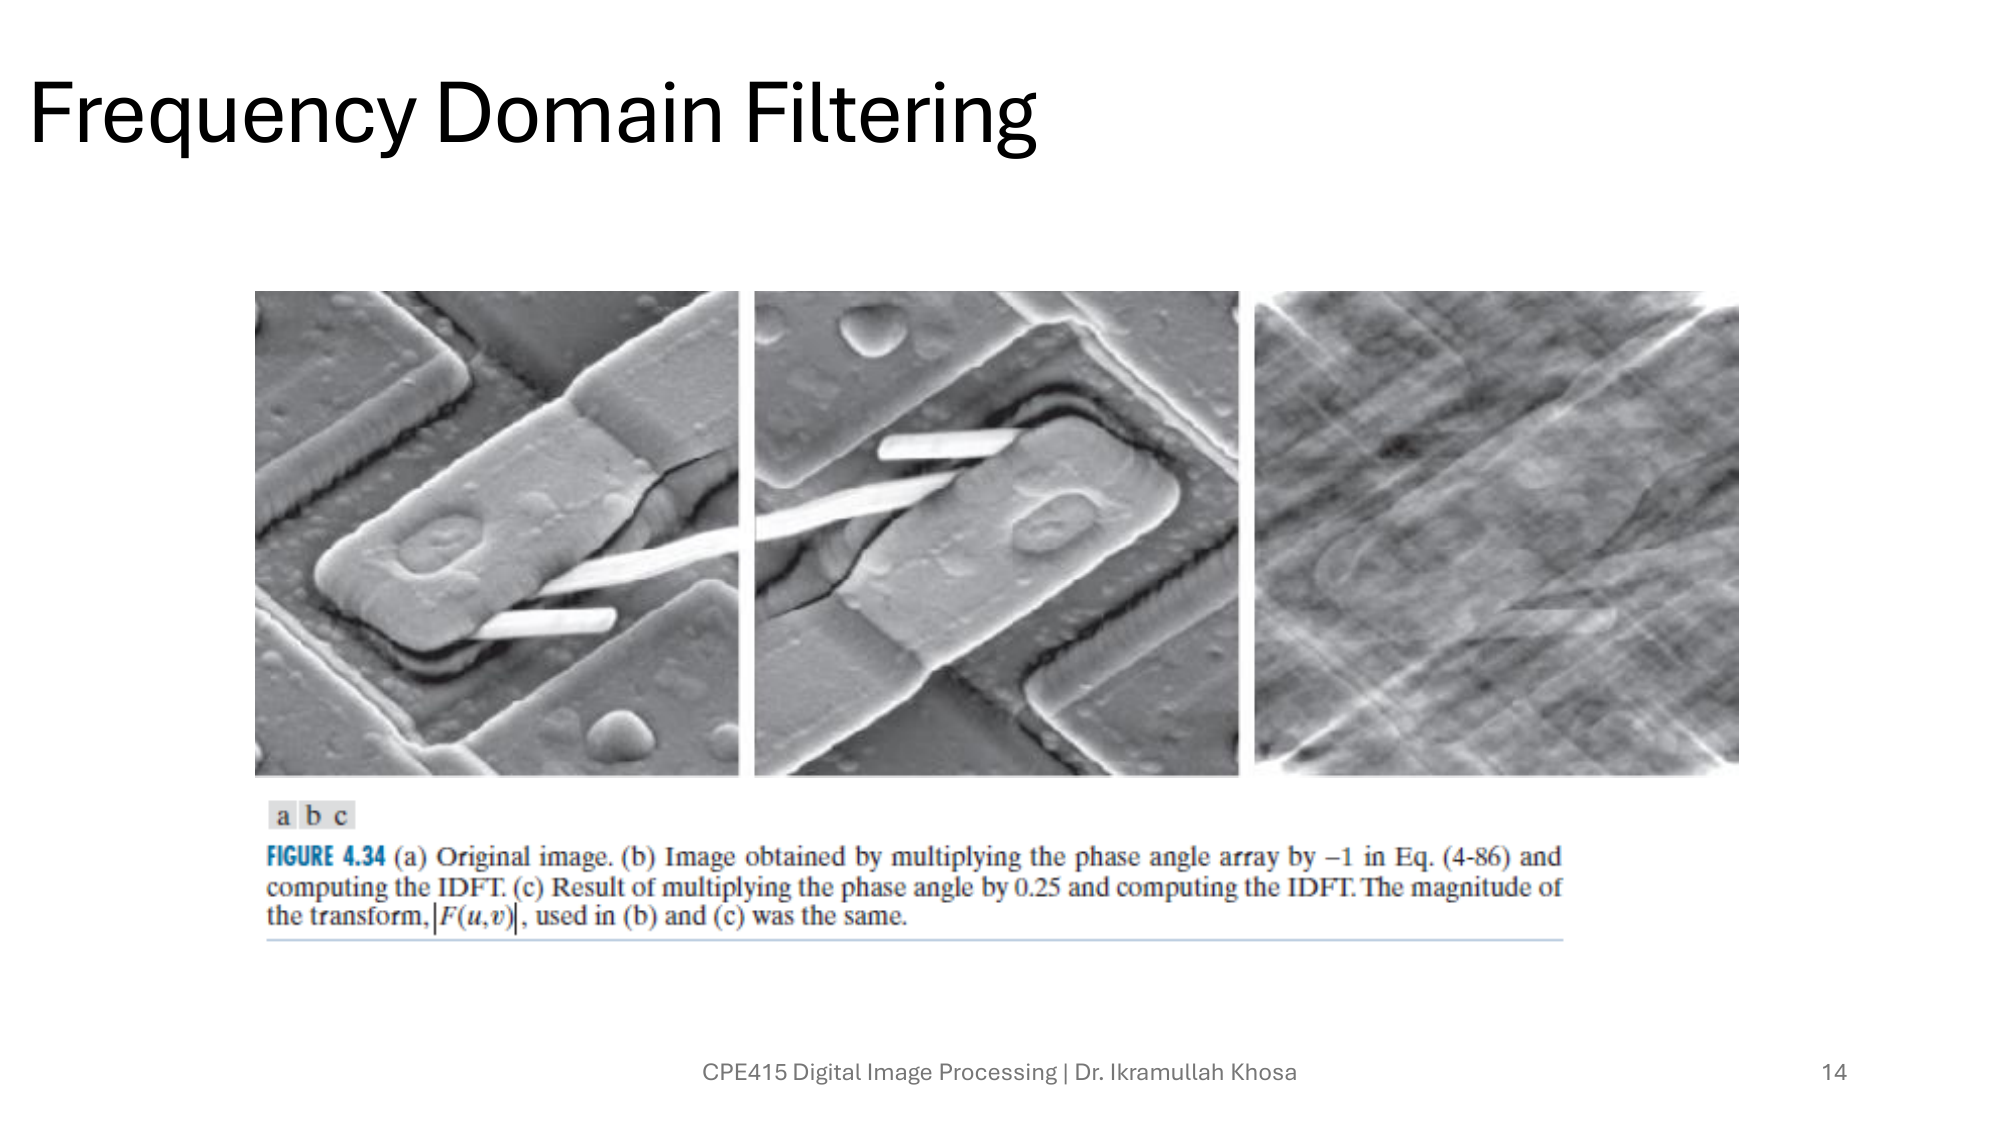
\includegraphics[width=0.95\textwidth]{images/slide9-14.png}
    \caption{Phase angle modification effects on SEM image (FIGURE 4.34)}
    \label{fig:phase_modification}
\end{figure}

\begin{deepexplanation}
\textbf{DEEP ANALYSIS - Figure \ref{fig:phase_modification}: The Critical Importance of Phase}

\textbf{What the Figure Shows (FIGURE 4.34):}
This striking demonstration shows what happens when you modify only the phase angles of an image's Fourier transform while keeping the magnitude unchanged:
\begin{itemize}
    \item \textbf{(a) Original SEM image}: The intact integrated circuit image with clear structural details
    \item \textbf{(b) Phase multiplied by $-1$}: All phase angles negated, equivalent to computing $F(u,v)^*$ (complex conjugate), then IDFT
    \item \textbf{(c) Phase multiplied by $0.25$}: Phase angles compressed to one-quarter of original values
\end{itemize}

\textbf{Key Observation:}
The magnitude $|F(u,v)|$ is \textbf{identical} in all three cases! Only the phase was modified.

\textbf{Why Results Differ So Dramatically:}
\begin{enumerate}
    \item \textbf{Negating phase (b)}: Creates a mirror-reversed image because $\mathcal{F}^{-1}\{F^*\} = f(-x, -y)$
    \item \textbf{Compressing phase (c)}: Severely degrades the image, creating a washed-out, ghostly appearance where edges and structures become indistinct
\end{enumerate}

\textbf{The Phase Paradox:}
\begin{itemize}
    \item \textbf{Magnitude} tells you \textit{how much} of each frequency is present (the ``energy'' distribution)
    \item \textbf{Phase} tells you \textit{where} each frequency component is located spatially
    \item \textbf{Conclusion}: Phase carries the structural information --- edges, textures, shapes all depend critically on correct phase relationships
\end{itemize}

\textbf{Practical Implications:}
\begin{itemize}
    \item Filtering operations that preserve phase (like lowpass/highpass) maintain image structure
    \item Phase corruption destroys recognizability even with perfect magnitude
    \item This is why phase-preserving algorithms are crucial in image processing
    \item Human vision is more sensitive to phase than magnitude distortions
\end{itemize}
\end{deepexplanation}

\begin{figure}[H]
    \centering
    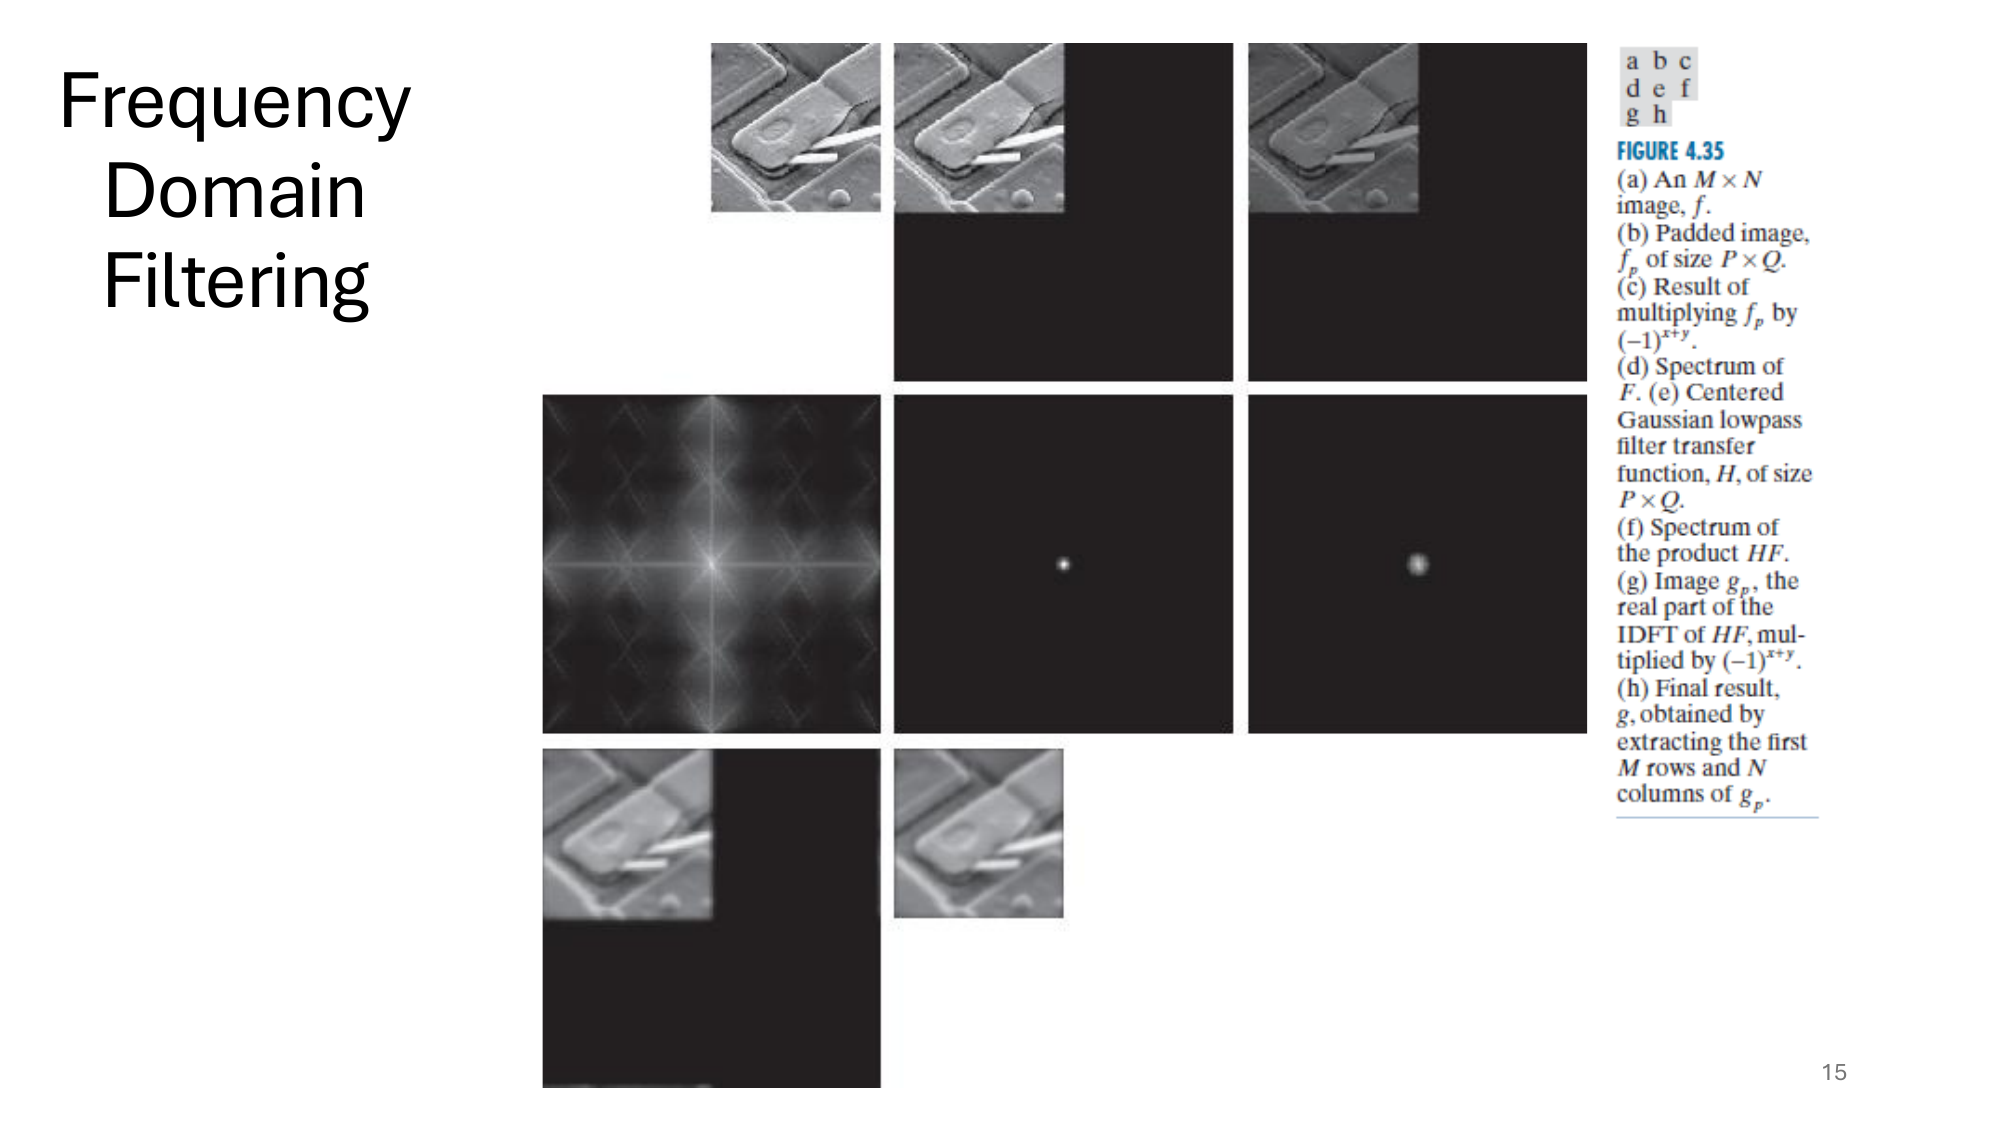
\includegraphics[width=0.95\textwidth]{images/slide9-15.png}
    \caption{Complete frequency domain filtering workflow with Gaussian lowpass (FIGURE 4.35)}
    \label{fig:filtering_workflow}
\end{figure}

\begin{deepexplanation}
\textbf{DEEP ANALYSIS - Figure \ref{fig:filtering_workflow}: Step-by-Step Filtering Process}

\textbf{What the Figure Shows (FIGURE 4.35):}
This comprehensive figure demonstrates the complete 8-step frequency domain filtering procedure applied to an SEM image using a Gaussian lowpass filter:

\textbf{Step-by-Step Breakdown:}
\begin{enumerate}
    \item \textbf{(a) Original image $f$}: The $M \times N$ SEM image of an integrated circuit
    
    \item \textbf{(b) Padded image $f_p$}: Image zero-padded to size $P \times Q$ (typically $P = 2M$, $Q = 2N$) to prevent wraparound artifacts
    
    \item \textbf{(c) Centered image}: Result of multiplying $f_p$ by $(-1)^{x+y}$, which shifts the DC component to the center of the spectrum
    
    \item \textbf{(d) Spectrum of $F$}: The 2D DFT showing the centered frequency spectrum with DC in the middle, bright spots indicating dominant frequencies
    
    \item \textbf{(e) Filter $H$}: The centered Gaussian lowpass transfer function of size $P \times Q$, appearing as a bright central disk that smoothly fades to black
    
    \item \textbf{(f) Product $HF$}: The filtered spectrum --- multiplication in frequency domain attenuates high frequencies (outer regions become darker)
    
    \item \textbf{(g) Filtered padded image $g_p$}: Real part of IDFT of $HF$, multiplied by $(-1)^{x+y}$ to uncenter, showing the blurred padded result
    
    \item \textbf{(h) Final result $g$}: Extracting the first $M$ rows and $N$ columns of $g_p$ gives the final filtered image
\end{enumerate}

\textbf{Critical Observations:}
\begin{itemize}
    \item The spectrum (d) shows diagonal bright lines corresponding to the edges in the IC image
    \item After filtering (f), these high-frequency components are significantly attenuated
    \item The final result (h) shows smoothed/blurred version with noise reduction
    \item Padding prevents the circular convolution artifacts that would otherwise appear
\end{itemize}

\textbf{Why Each Step Matters:}
\begin{itemize}
    \item \textbf{Padding}: Without it, features from opposite edges would ``wrap around''
    \item \textbf{Centering}: Makes filter design intuitive (low frequencies in center)
    \item \textbf{Cropping}: Returns image to original size, discarding padding artifacts
\end{itemize}
\end{deepexplanation}

%==============================================================================
\section{Highpass Filters: Edge Enhancement}
%==============================================================================

Highpass filters attenuate low frequencies, enhancing edges and fine details.

\begin{mathbox}
\textbf{Highpass from Lowpass:}
\[
H_{HP}(u, v) = 1 - H_{LP}(u, v)
\]
This relationship holds for all three filter types.
\end{mathbox}

\begin{figure}[H]
    \centering
    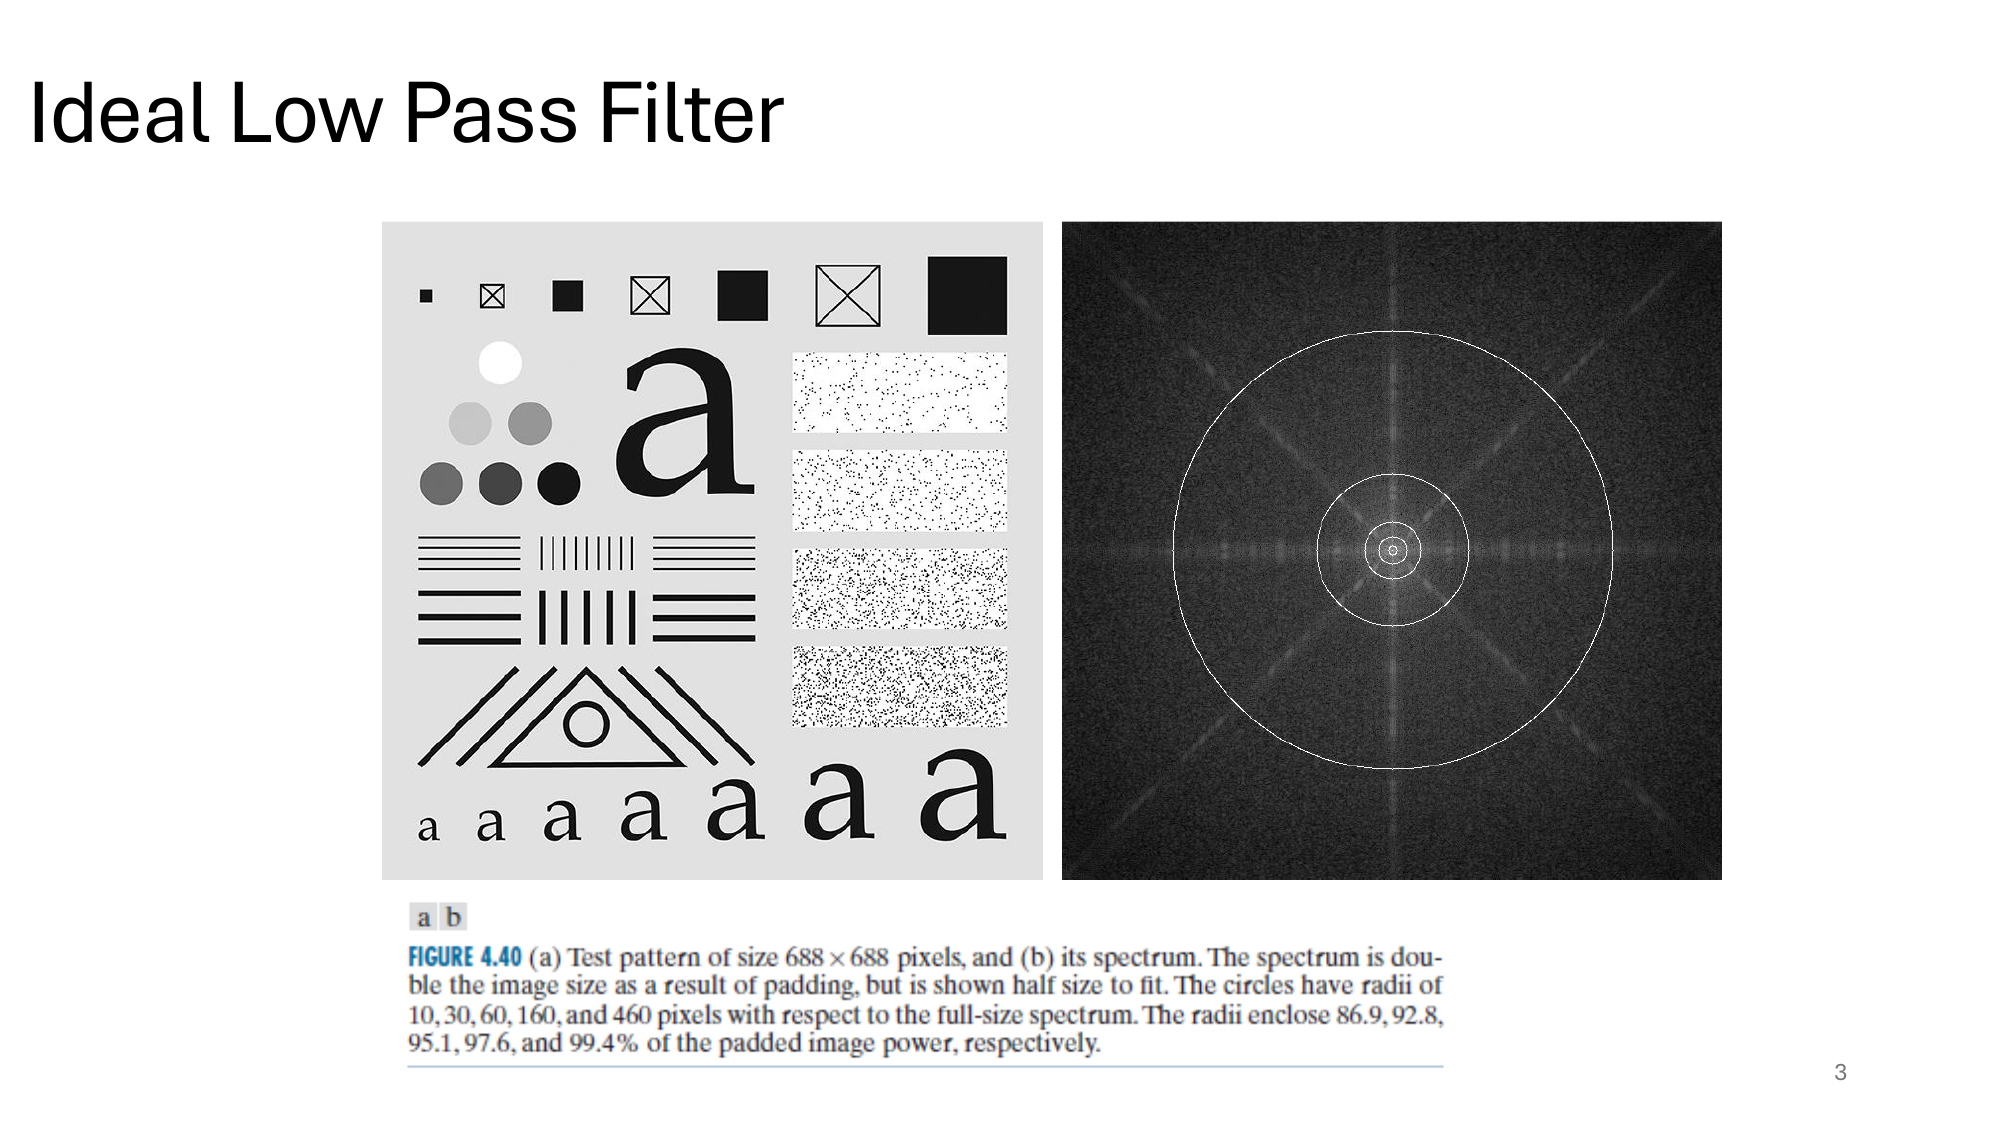
\includegraphics[width=0.85\textwidth]{images/slide10-03.png}
    \caption{Test pattern showing percentage of total image power enclosed by circles of various radii}
    \label{fig:power_circles}
\end{figure}

\begin{deepexplanation}
\textbf{DEEP ANALYSIS - Figure \ref{fig:power_circles}: Understanding Filter Cutoff Selection}

\textbf{What This Figure Shows:}
This is a test pattern image with its Fourier spectrum, annotated with concentric circles indicating how much of the total image power (energy) is contained within each radius from the DC component.

\textbf{Power Spectrum Distribution:}
\begin{itemize}
    \item The numbers on each circle indicate the percentage of total power enclosed
    \item Most natural images have power concentrated near the center (low frequencies)
    \item The DC component alone often contains 90\%+ of total power
    \item High-frequency components contribute relatively little power
\end{itemize}

\textbf{Why This Matters for Filter Design:}
\begin{itemize}
    \item Helps choose appropriate cutoff frequency $D_0$
    \item If $D_0$ encloses 95\% of power, only 5\% is removed (mild smoothing)
    \item If $D_0$ encloses 80\% of power, 20\% is removed (significant smoothing)
    \item Trade-off: More power removed = more blur but less noise
\end{itemize}

\textbf{Practical Application:}
\begin{enumerate}
    \item Compute spectrum of image
    \item Calculate cumulative power as function of radius
    \item Choose $D_0$ based on desired power retention percentage
    \item Design filter with that cutoff
\end{enumerate}

\textbf{Important Insight:}
Because power is concentrated at low frequencies, even aggressive lowpass filtering (removing frequencies beyond a small radius) preserves most image information. This explains why blurring removes noise effectively while retaining recognizable structure.
\end{deepexplanation}

\begin{figure}[H]
    \centering
    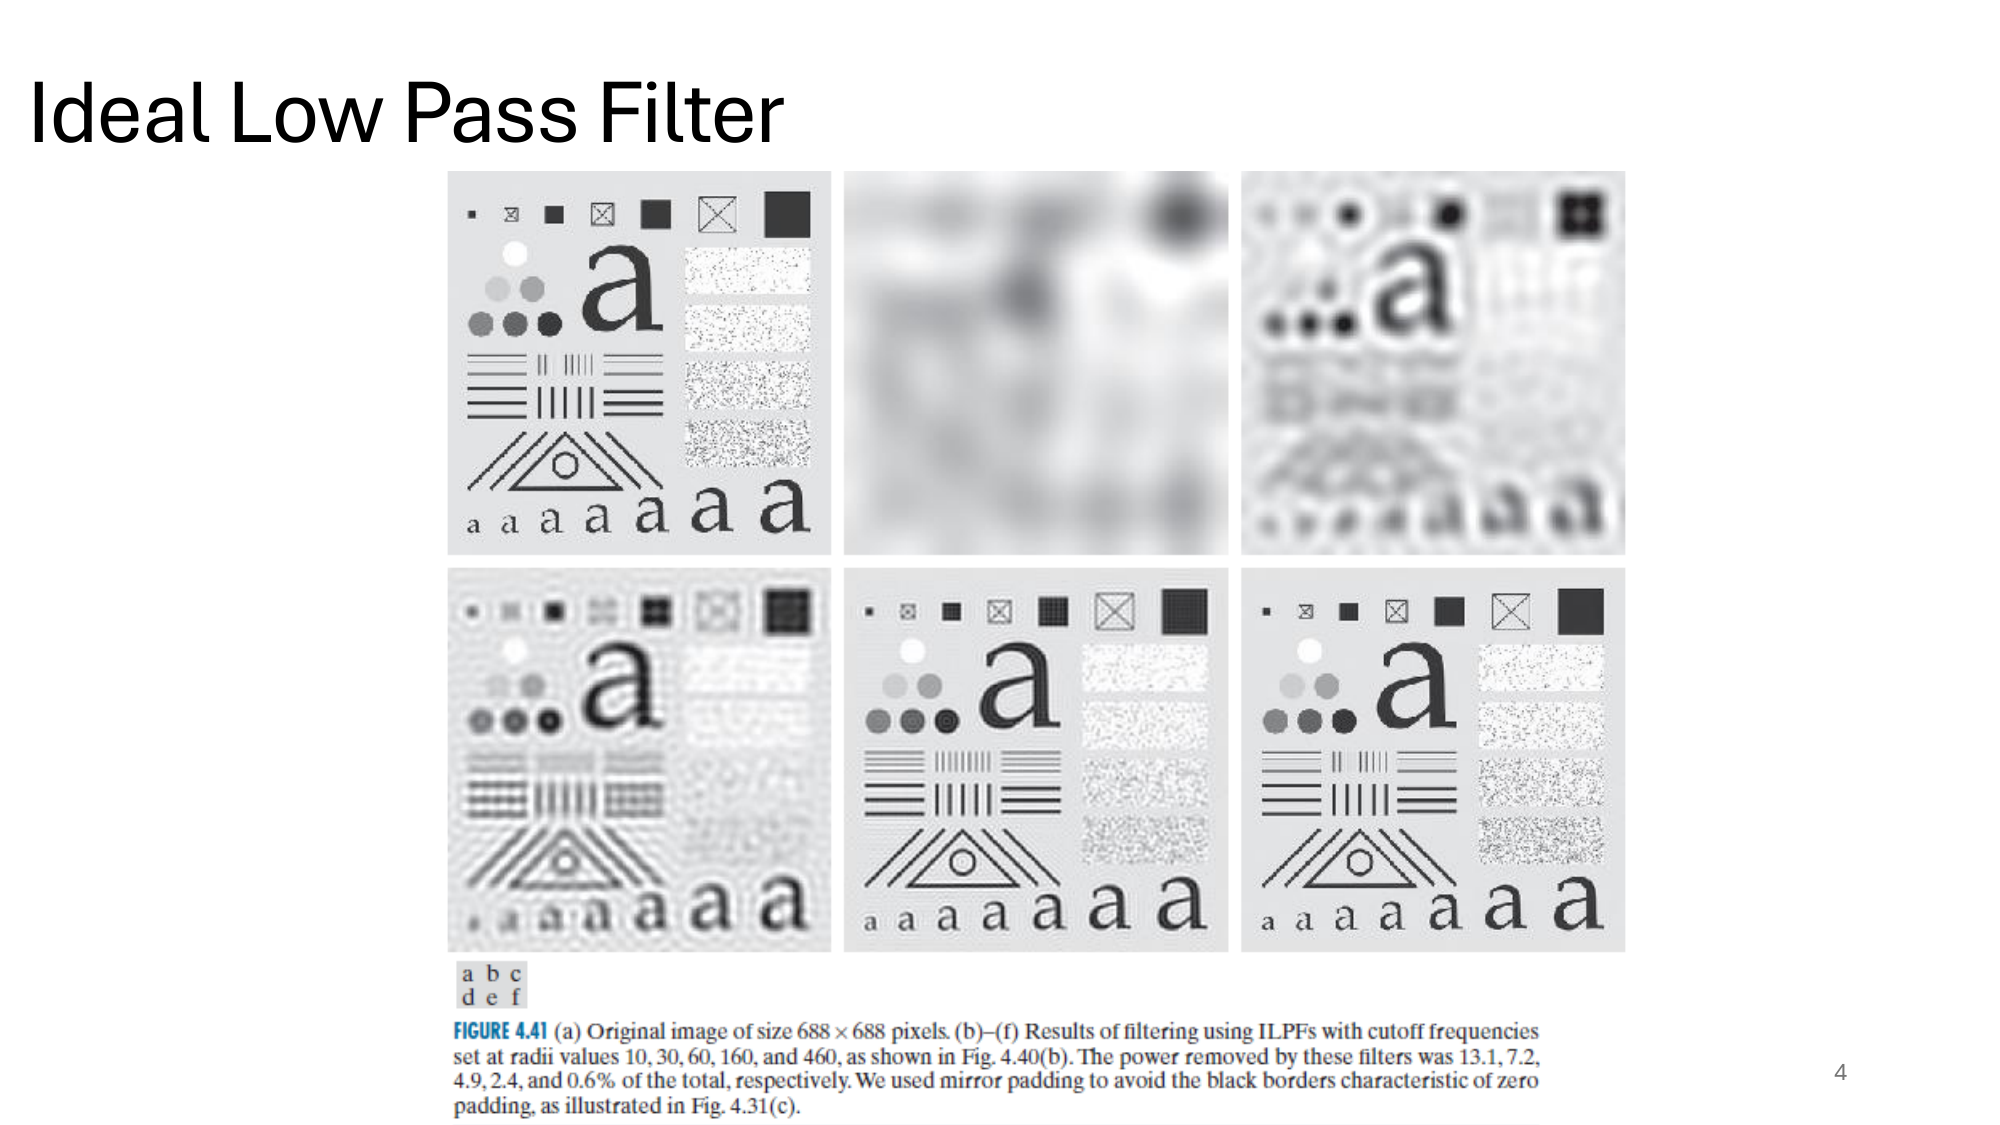
\includegraphics[width=0.9\textwidth]{images/slide10-04.png}
    \caption{Ideal lowpass filtering results at different cutoff frequencies showing ringing artifacts}
    \label{fig:ilpf_results}
\end{figure}

\begin{deepexplanation}
\textbf{DEEP ANALYSIS - Figure \ref{fig:ilpf_results}: Effects of Ideal Lowpass Filter Cutoff}

\textbf{What This Figure Demonstrates:}
A series of filtered images using the Ideal Lowpass Filter (ILPF) with progressively larger cutoff radii $D_0$. Each panel shows the result of filtering with a different cutoff value.

\textbf{Key Observations:}
\begin{itemize}
    \item Small $D_0$: Heavy blur, removes most detail, visible ringing artifacts
    \item Medium $D_0$: Moderate smoothing, some ringing around edges
    \item Large $D_0$: Minimal smoothing, approaches original image
\end{itemize}

\textbf{Ringing Artifacts (Gibbs Phenomenon):}
The sharp cutoff of the ideal filter creates sinc-function oscillations in the spatial domain. This manifests as:
\begin{itemize}
    \item Concentric rings around high-contrast edges
    \item ``Halos'' around bright objects
    \item Overshoot and undershoot near discontinuities
\end{itemize}

\textbf{Why Ringing Occurs:}
The ideal filter's rectangular frequency response has an infinite-extent sinc function as its spatial impulse response. Convolution with this sinc creates the oscillatory artifacts.

\textbf{Practical Implication:}
Despite its mathematically clean definition, the ideal lowpass filter is rarely used in practice due to these ringing artifacts. Butterworth and Gaussian filters provide smoother transitions that avoid this problem.
\end{deepexplanation}

\subsection{High-Frequency Emphasis and Unsharp Masking}

Pure highpass filtering removes the average brightness (DC), making images hard to view. High-frequency emphasis adds back the low frequencies:

\begin{mathbox}
\textbf{High-Frequency Emphasis:}
\[
H_{HFE}(u, v) = k_1 + k_2 \cdot H_{HP}(u, v)
\]
where $k_1 \geq 0$ is the DC offset and $k_2 \geq 0$ controls emphasis strength.

Common choice: $k_1 = 1, k_2 = 1$ gives $H_{HFE} = 1 + H_{HP}$
\end{mathbox}

\begin{figure}[H]
    \centering
    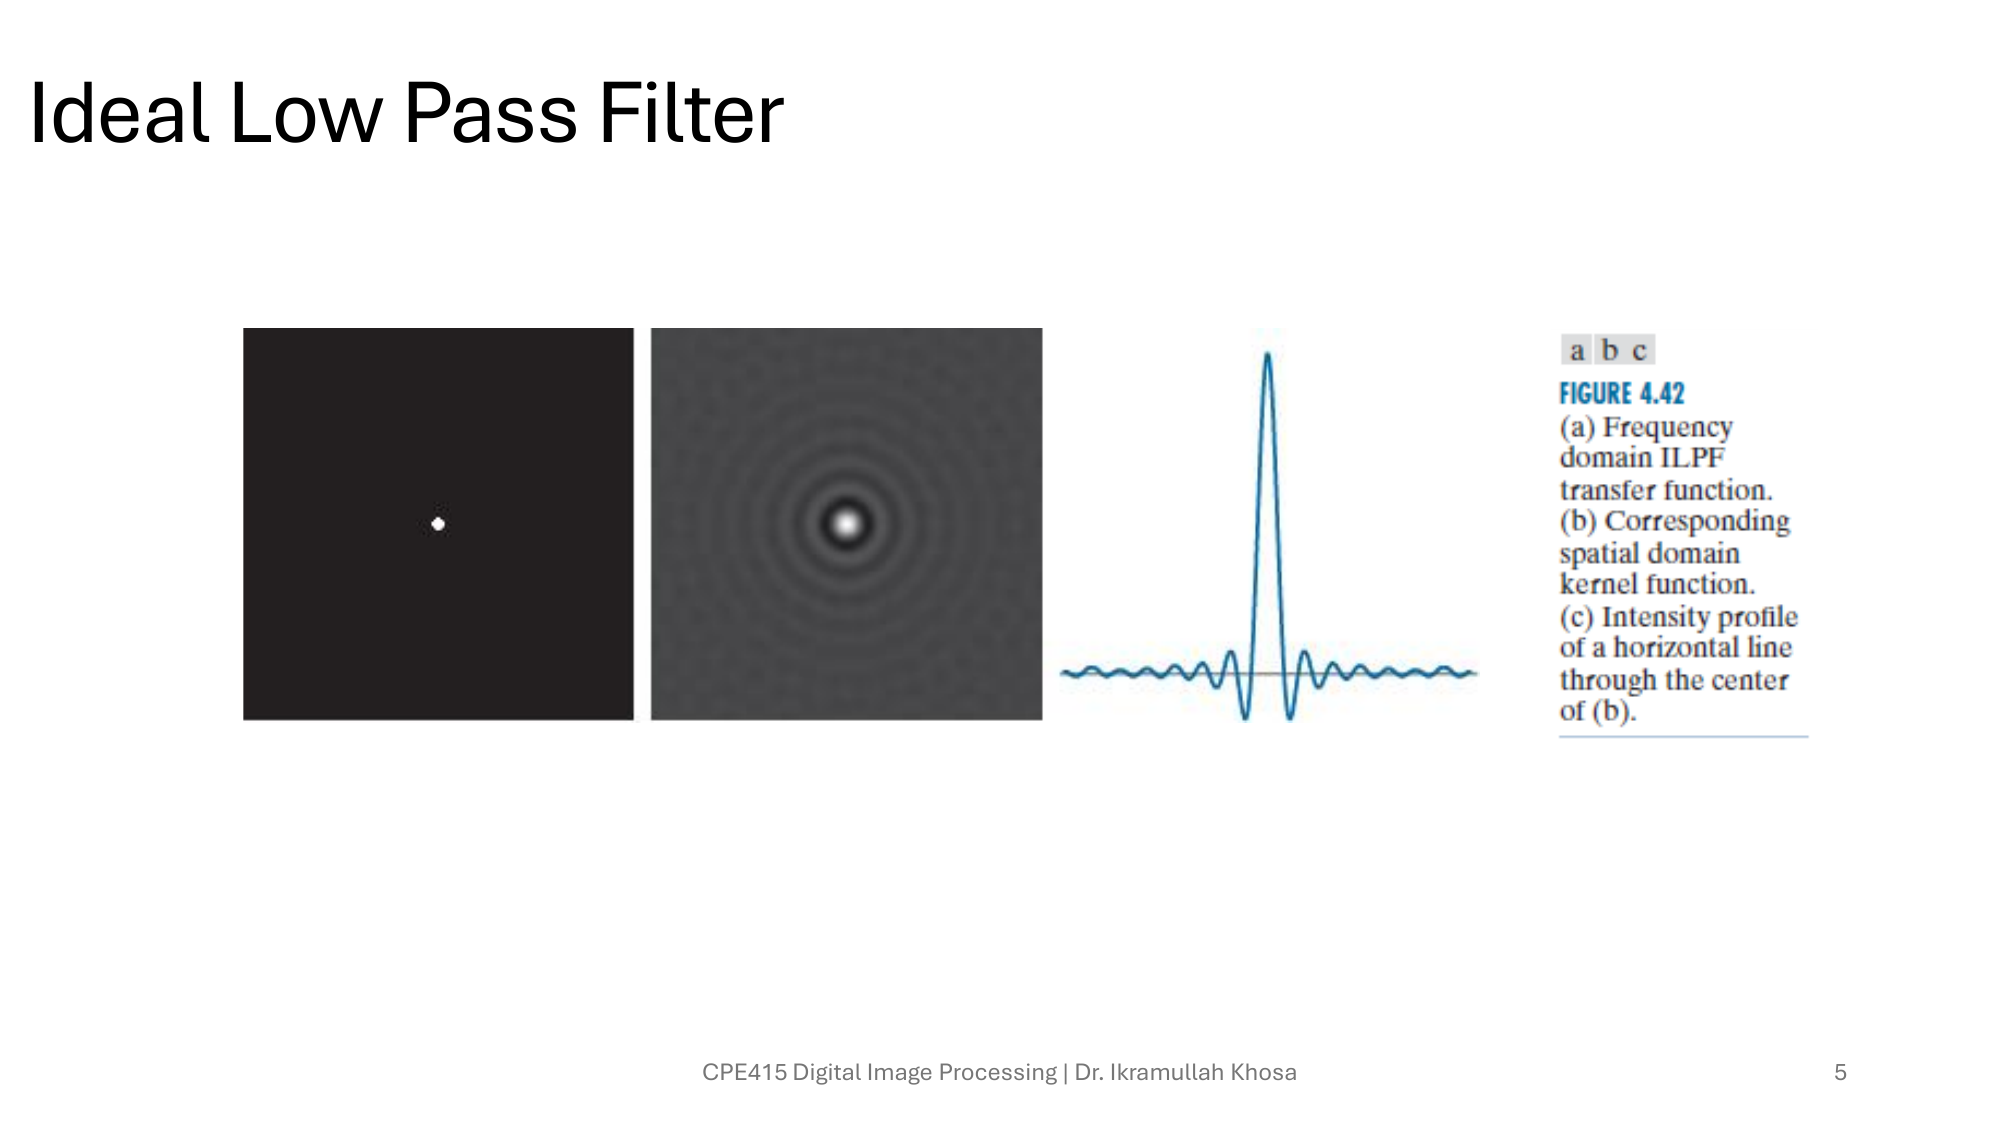
\includegraphics[width=0.9\textwidth]{images/slide10-05.png}
    \caption{Butterworth lowpass filter: 3D perspective plot showing smooth frequency response}
    \label{fig:blpf_perspective}
\end{figure}

\begin{deepexplanation}
\textbf{DEEP ANALYSIS - Figure \ref{fig:blpf_perspective}: Butterworth Lowpass Filter Shape}

\textbf{What This Figure Shows:}
A three-dimensional perspective view of the Butterworth lowpass filter transfer function $H(u,v)$, displaying its characteristic smooth, bell-shaped profile centered at the origin.

\textbf{Butterworth LPF Definition:}
\[
H(u, v) = \frac{1}{1 + \left[\frac{D(u, v)}{D_0}\right]^{2n}}
\]
where $D(u,v) = \sqrt{u^2 + v^2}$, $D_0$ is cutoff frequency, and $n$ is filter order.

\textbf{Key Visual Features:}
\begin{itemize}
    \item Peak value of 1 at center (DC passes unchanged)
    \item Smooth roll-off toward edges (no sharp transitions)
    \item Circularly symmetric shape
    \item At $D = D_0$: $H = 0.5$ (half-power point, defining cutoff)
\end{itemize}

\textbf{Why the Smooth Shape Matters:}
\begin{itemize}
    \item No abrupt frequency cutoff → No ringing in spatial domain
    \item Higher order $n$ → Steeper transition but still smooth
    \item Trade-off: Sharper frequency selectivity vs. spatial artifacts
\end{itemize}

\textbf{Comparison with Ideal LPF:}
The ideal filter would be a flat-topped cylinder (1 inside $D_0$, 0 outside). The Butterworth's smooth roll-off eliminates the Gibbs phenomenon while maintaining good frequency selectivity.
\end{deepexplanation}

\begin{figure}[H]
    \centering
    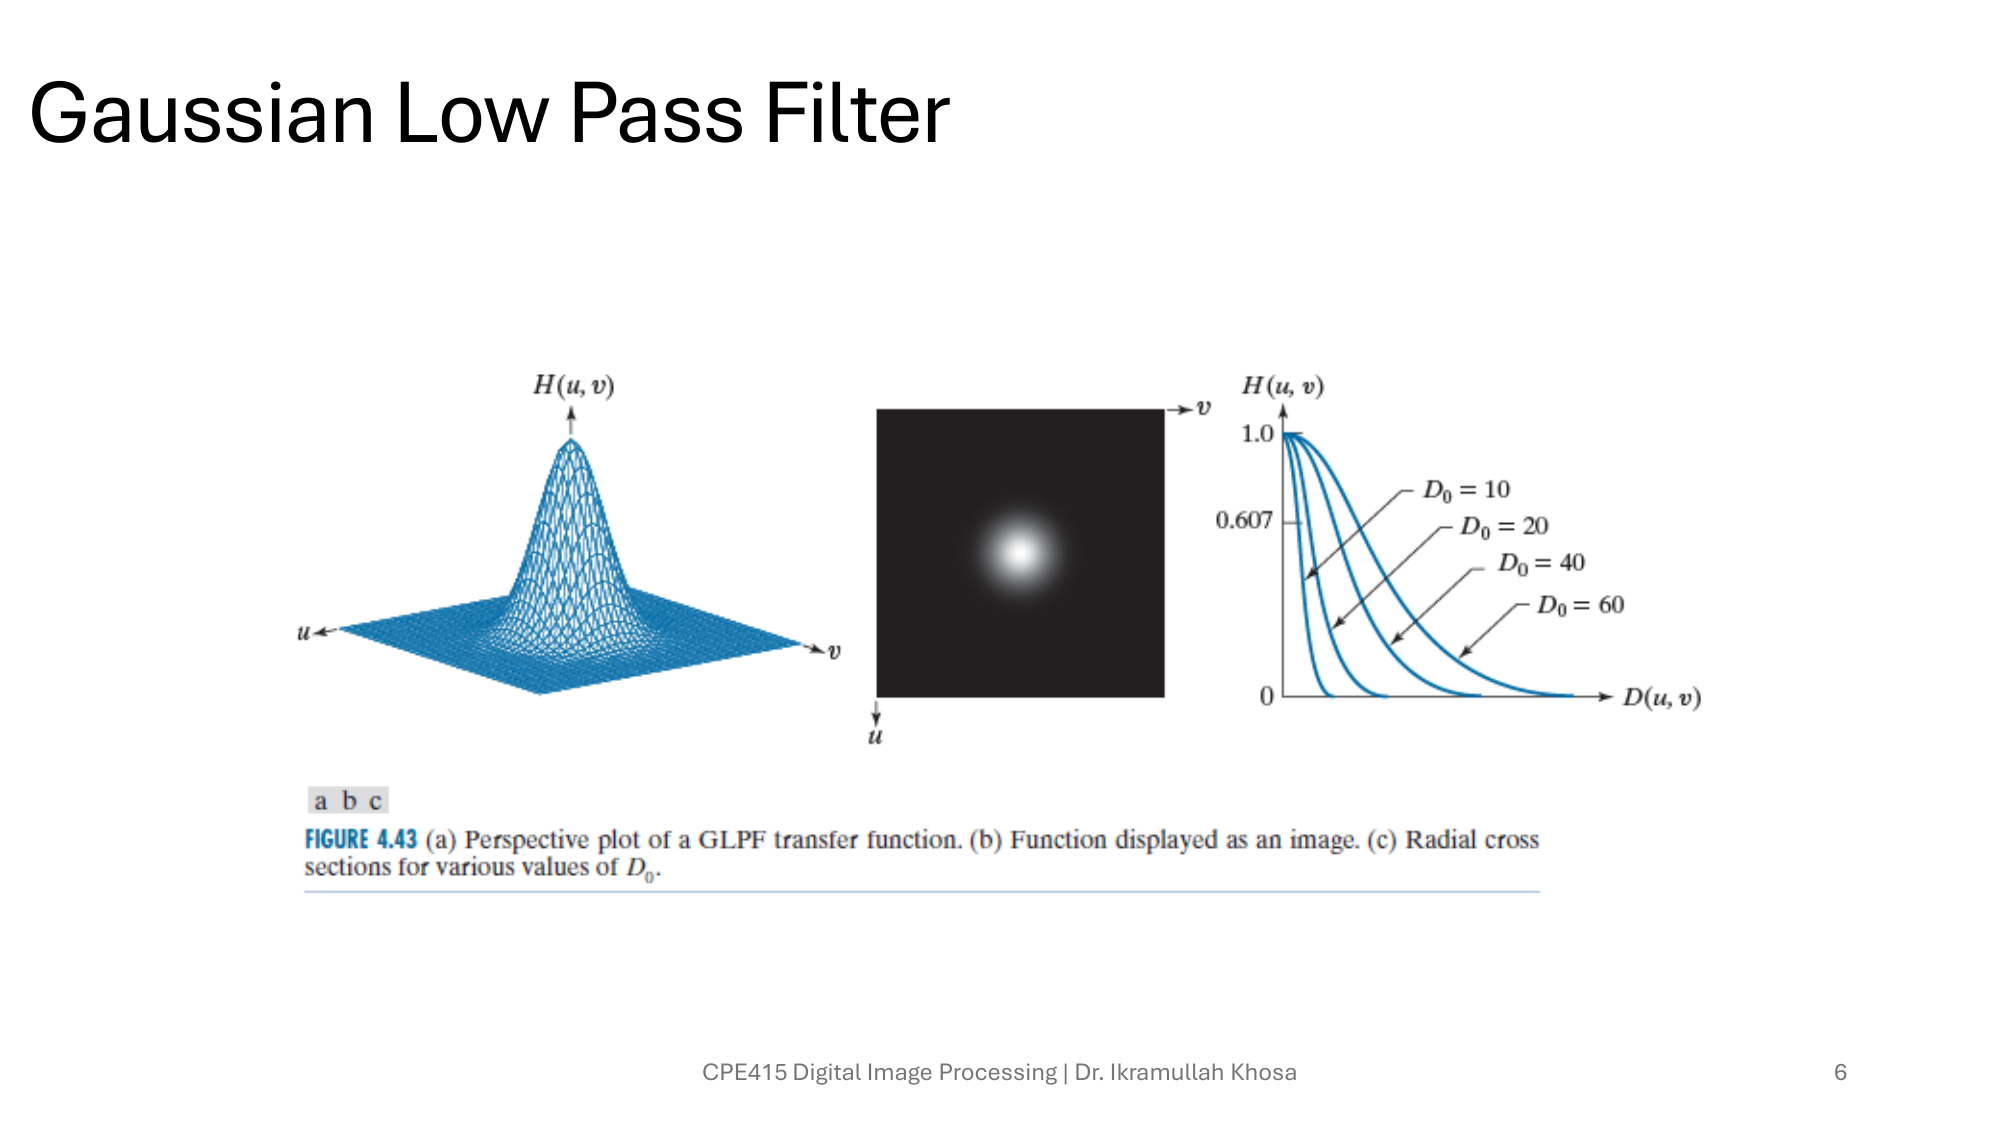
\includegraphics[width=0.9\textwidth]{images/slide10-06.png}
    \caption{Butterworth lowpass filtering results at different cutoff frequencies}
    \label{fig:blpf_results}
\end{figure}

\begin{deepexplanation}
\textbf{DEEP ANALYSIS - Figure \ref{fig:blpf_results}: Butterworth LPF Applied to Images}

\textbf{What This Figure Shows:}
A comparison of Butterworth lowpass filtering results on a test image at various cutoff frequencies $D_0$, demonstrating the filter's smoothing effect without the ringing artifacts of the ideal filter.

\textbf{Key Observations:}
\begin{itemize}
    \item Small $D_0$: Strong smoothing, significant blur, but NO ringing
    \item Medium $D_0$: Moderate smoothing, detail preserved
    \item Large $D_0$: Minimal effect, approaches original
\end{itemize}

\textbf{Comparison with Ideal LPF Results:}
At the same cutoff frequency:
\begin{itemize}
    \item ILPF: Sharp edges but visible ringing halos
    \item BLPF: Slightly softer edges but clean, artifact-free
\end{itemize}

\textbf{Effect of Filter Order $n$:}
\begin{itemize}
    \item $n = 1$: Very gradual transition, maximum smoothness
    \item $n = 2$: Good balance of selectivity and smoothness
    \item $n = 4$: Sharper transition, approaches ideal but no ringing
    \item $n \to \infty$: Approaches ideal filter behavior
\end{itemize}

\textbf{Practical Application:}
Butterworth filters are widely used because they provide predictable, controllable smoothing without introducing artificial artifacts. The order parameter allows fine-tuning of the sharpness/smoothness trade-off.
\end{deepexplanation}


%==============================================================================
\section{Selective Filtering: Bandpass, Bandreject, and Notch}
%==============================================================================

Sometimes we need to target specific frequency ranges rather than simply low or high frequencies.

\subsection{Bandreject (Notch) Filters}

\begin{mathbox}
\textbf{Ideal Bandreject Filter:}
\[
H(u, v) = \begin{cases} 0 & D_0 - W/2 \leq D(u, v) \leq D_0 + W/2 \\ 1 & \text{otherwise} \end{cases}
\]
where $D_0$ is the center of the reject band and $W$ is its width.
\end{mathbox}

\begin{figure}[H]
    \centering
    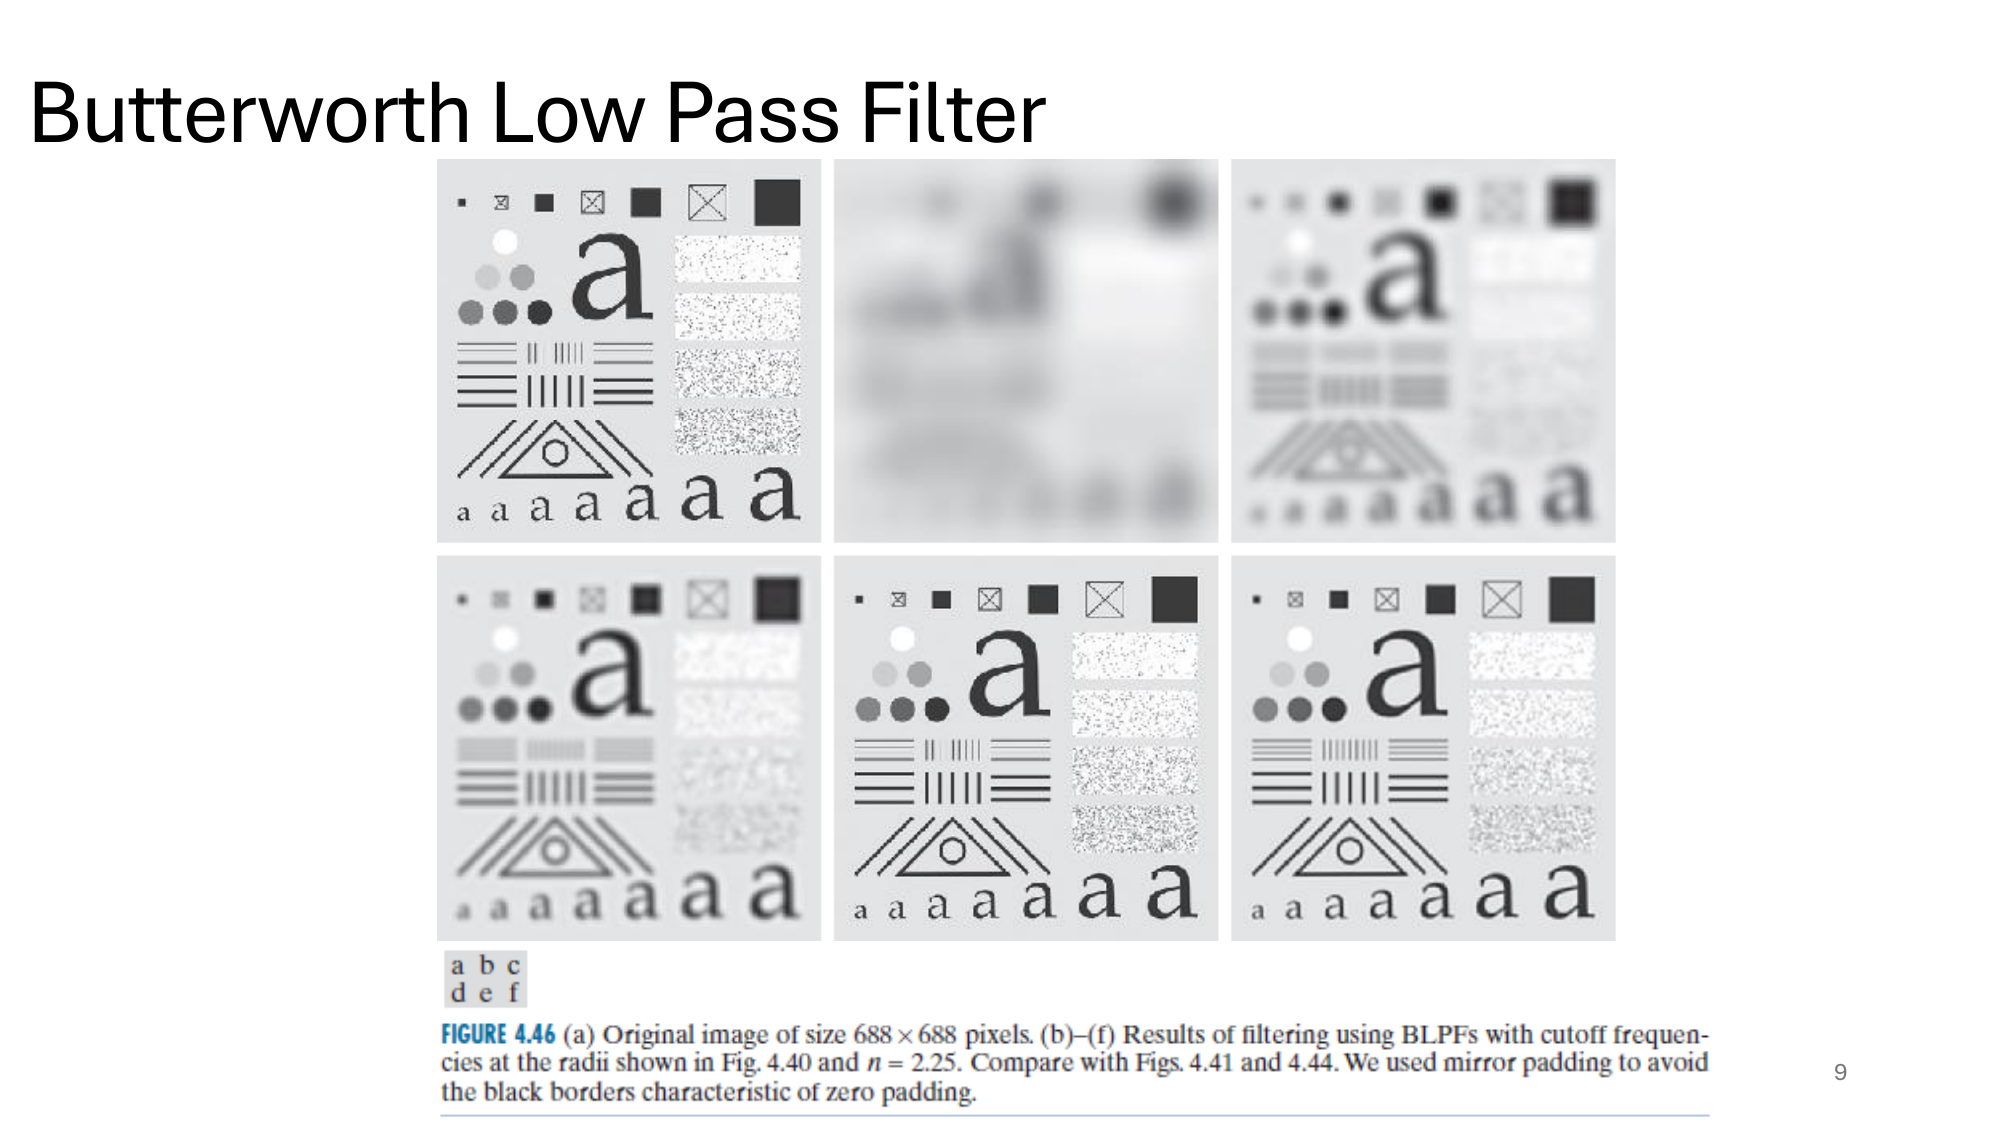
\includegraphics[width=0.85\textwidth]{images/slide10-09.png}
    \caption{Butterworth lowpass filter applied to test pattern at different cutoff frequencies}
    \label{fig:blpf_test_pattern}
\end{figure}

\begin{deepexplanation}
\textbf{DEEP ANALYSIS - Figure \ref{fig:blpf_test_pattern}: Butterworth LPF on Test Pattern}

\textbf{What This Figure Shows:}
A test pattern image filtered with Butterworth lowpass filters at various cutoff frequencies $D_0$, showing how different frequencies are selectively attenuated.

\textbf{Test Pattern Purpose:}
Test patterns contain known frequency components at specific locations, making it easy to visualize which frequencies pass through the filter:
\begin{itemize}
    \item Fine bars/gratings = High frequencies
    \item Coarse bars/gratings = Low frequencies
    \item Different orientations test all frequency directions
\end{itemize}

\textbf{What to Observe:}
\begin{itemize}
    \item Small $D_0$: Only large, coarse features remain visible
    \item Medium $D_0$: Medium details preserved, fine details blurred
    \item Large $D_0$: Most details preserved, minimal smoothing
\end{itemize}

\textbf{Comparison with ILPF:}
Unlike the ideal filter results, there is no visible ringing around the bars and edges of the pattern. The Butterworth filter's smooth transition eliminates these artifacts.

\textbf{Practical Insight:}
This demonstrates how cutoff frequency selection directly determines which image features are preserved. Understanding this relationship is crucial for choosing appropriate filter parameters in real applications.
\end{deepexplanation}

\subsection{Butterworth Spatial Impulse Response}

\begin{figure}[H]
    \centering
    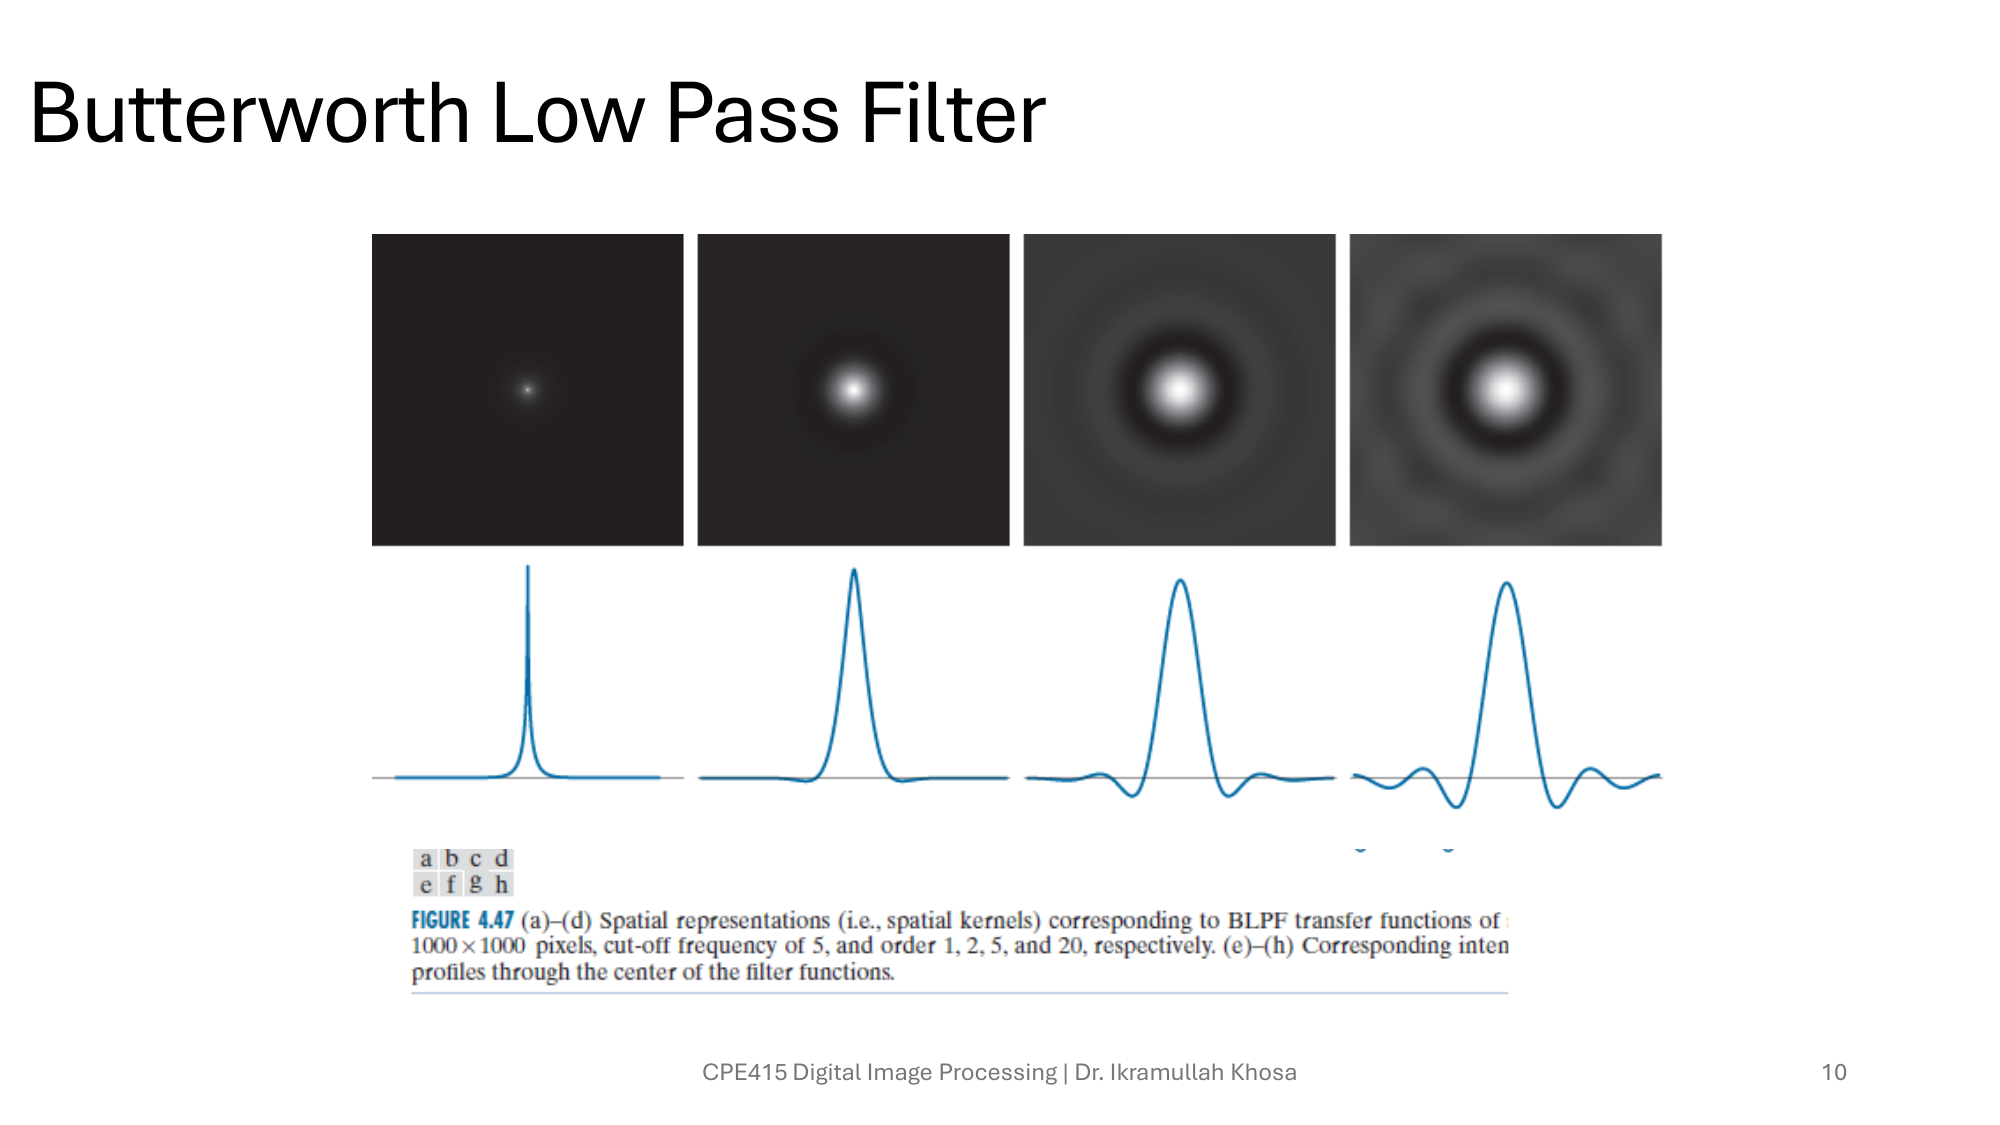
\includegraphics[width=0.9\textwidth]{images/slide10-10.png}
    \caption{Butterworth lowpass filter: spatial domain kernels and radial profiles for different orders}
    \label{fig:blpf_spatial}
\end{figure}

\begin{deepexplanation}
\textbf{DEEP ANALYSIS - Figure \ref{fig:blpf_spatial}: Spatial Domain Representation}

\textbf{What This Figure Shows:}
The spatial domain impulse responses (convolution kernels) of Butterworth lowpass filters at different orders, along with their radial intensity profiles.

\textbf{Key Visual Features:}
\begin{itemize}
    \item Central peak: Maximum value at the center
    \item Smooth decay: Gradual decrease toward edges
    \item Higher orders: More concentrated central lobe
    \item Circular symmetry: Same profile in all directions
\end{itemize}

\textbf{Relationship to Frequency Domain:}
The spatial kernel is the inverse Fourier transform of the frequency response:
\[
h(x, y) = \mathcal{F}^{-1}\{H(u, v)\}
\]
Smoother frequency transitions → more compact spatial kernels → less ringing.

\textbf{Order Effects on Spatial Kernel:}
\begin{itemize}
    \item $n = 1$: Broadest kernel, most blurring per pixel
    \item $n = 2$: Moderate spread, good all-purpose choice
    \item Higher $n$: More concentrated, approaching sinc-like behavior
\end{itemize}

\textbf{Practical Significance:}
Understanding the spatial kernel helps visualize what ``smoothing'' actually does: it replaces each pixel with a weighted average of its neighbors, with the kernel defining the weights.
\end{deepexplanation}

\subsection{Lowpass Filter Transfer Functions Summary}

\begin{figure}[H]
    \centering
    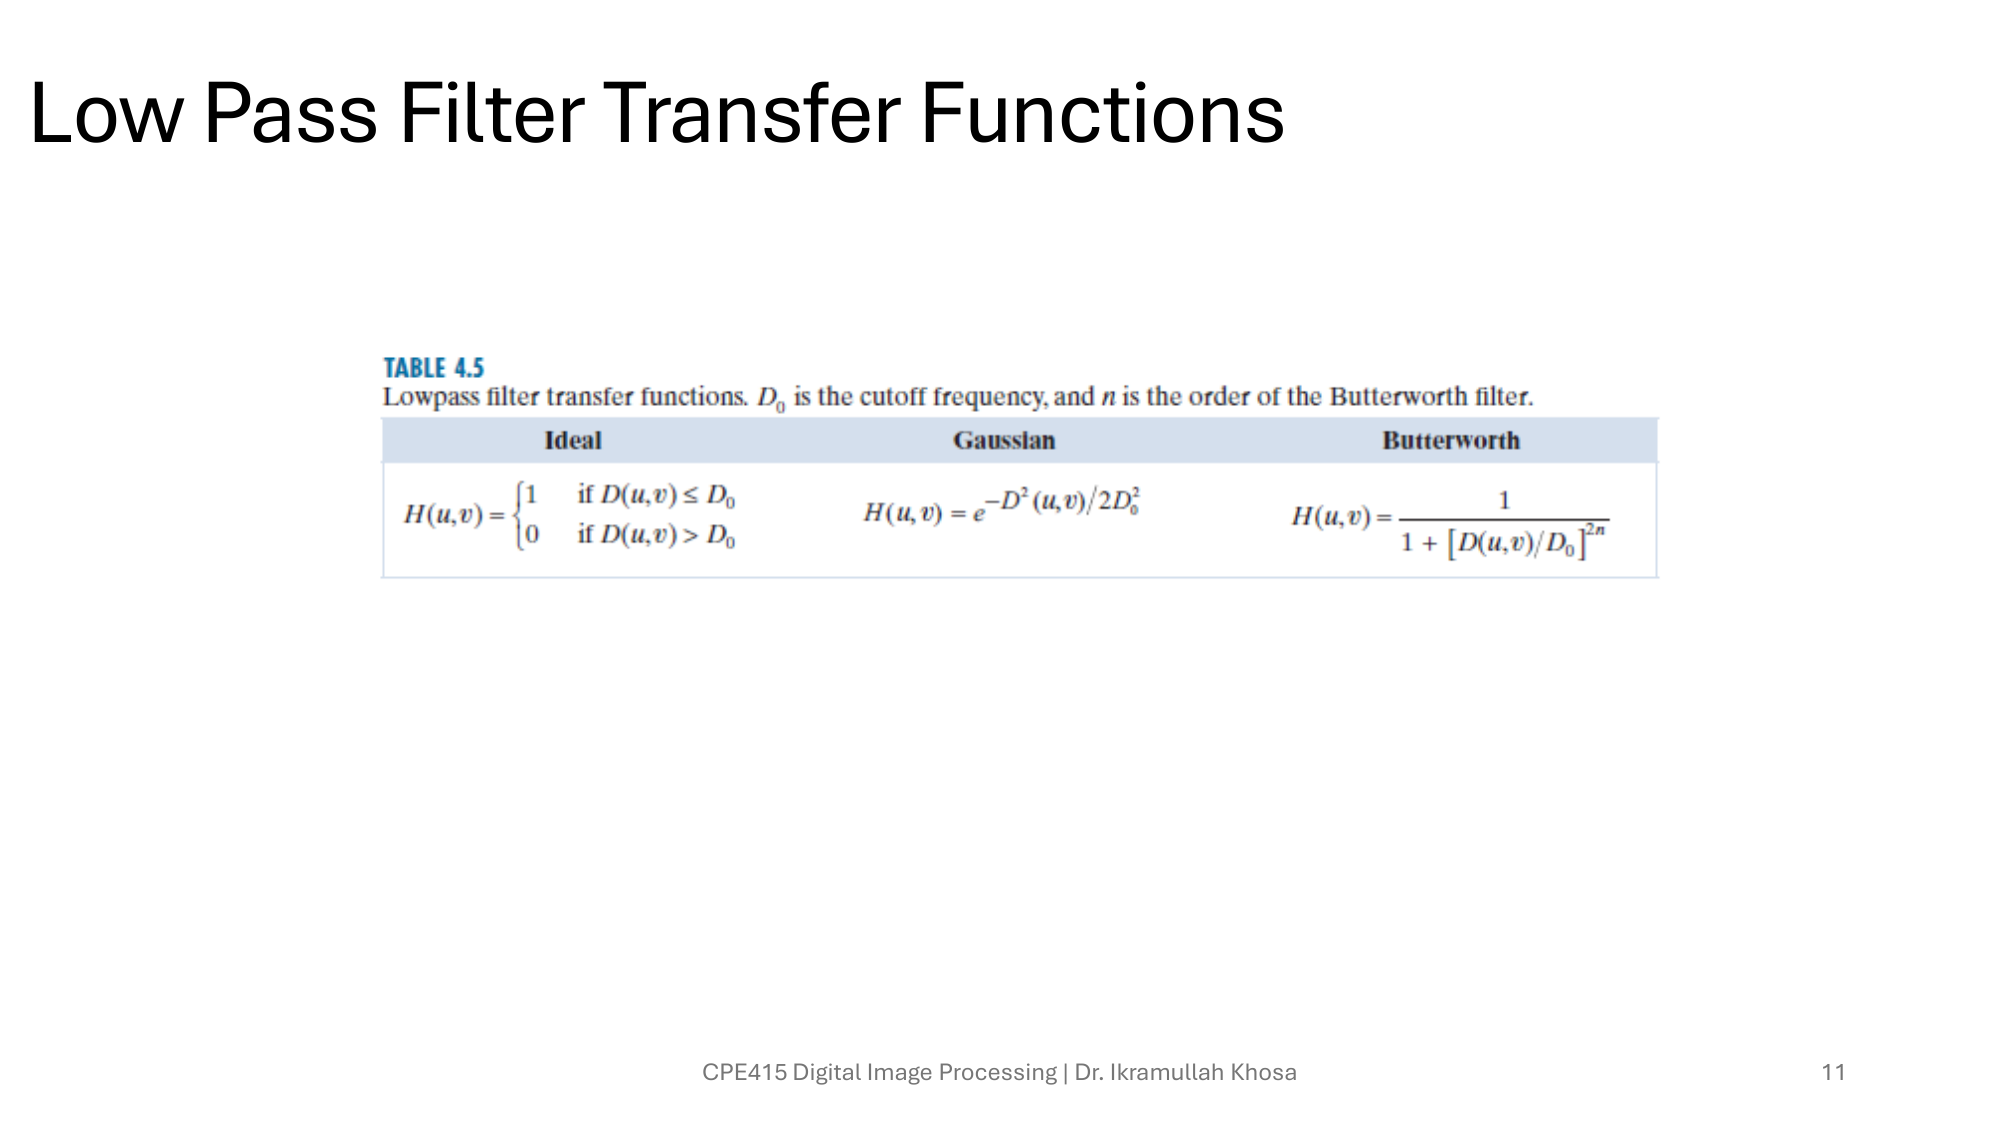
\includegraphics[width=0.95\textwidth]{images/slide10-11.png}
    \caption{Summary table of lowpass filter transfer functions: Ideal, Butterworth, and Gaussian}
    \label{fig:lpf_table}
\end{figure}

\begin{deepexplanation}
\textbf{DEEP ANALYSIS - Figure \ref{fig:lpf_table}: Comparing Filter Definitions}

\textbf{What This Table Provides:}
A comprehensive comparison of the three main lowpass filter types, showing their mathematical definitions and key characteristics.

\textbf{Ideal Lowpass Filter (ILPF):}
\[
H(u, v) = \begin{cases} 1 & D(u, v) \leq D_0 \\ 0 & D(u, v) > D_0 \end{cases}
\]
\begin{itemize}
    \item Sharpest possible frequency cutoff
    \item Produces severe ringing artifacts
    \item Rarely used in practice
\end{itemize}

\textbf{Butterworth Lowpass Filter (BLPF):}
\[
H(u, v) = \frac{1}{1 + [D(u, v)/D_0]^{2n}}
\]
\begin{itemize}
    \item Smooth transition, adjustable via order $n$
    \item At $D = D_0$: $H = 0.5$ (half-power point)
    \item Most versatile choice for general use
\end{itemize}

\textbf{Gaussian Lowpass Filter (GLPF):}
\[
H(u, v) = e^{-D(u, v)^2 / 2\sigma^2}
\]
\begin{itemize}
    \item Smoothest possible transition
    \item No ringing whatsoever
    \item Self-similar: Gaussian in frequency → Gaussian in space
\end{itemize}

\textbf{Selection Guide:}
\begin{itemize}
    \item Need sharp cutoff with acceptable artifacts → ILPF
    \item Need controllable transition → BLPF with appropriate $n$
    \item Need maximum smoothness, no artifacts → GLPF
\end{itemize}
\end{deepexplanation}

\subsection{Notch Filters}

Notch filters are selective bandreject filters that target specific frequency locations (points), not rings.

\begin{figure}[H]
    \centering
    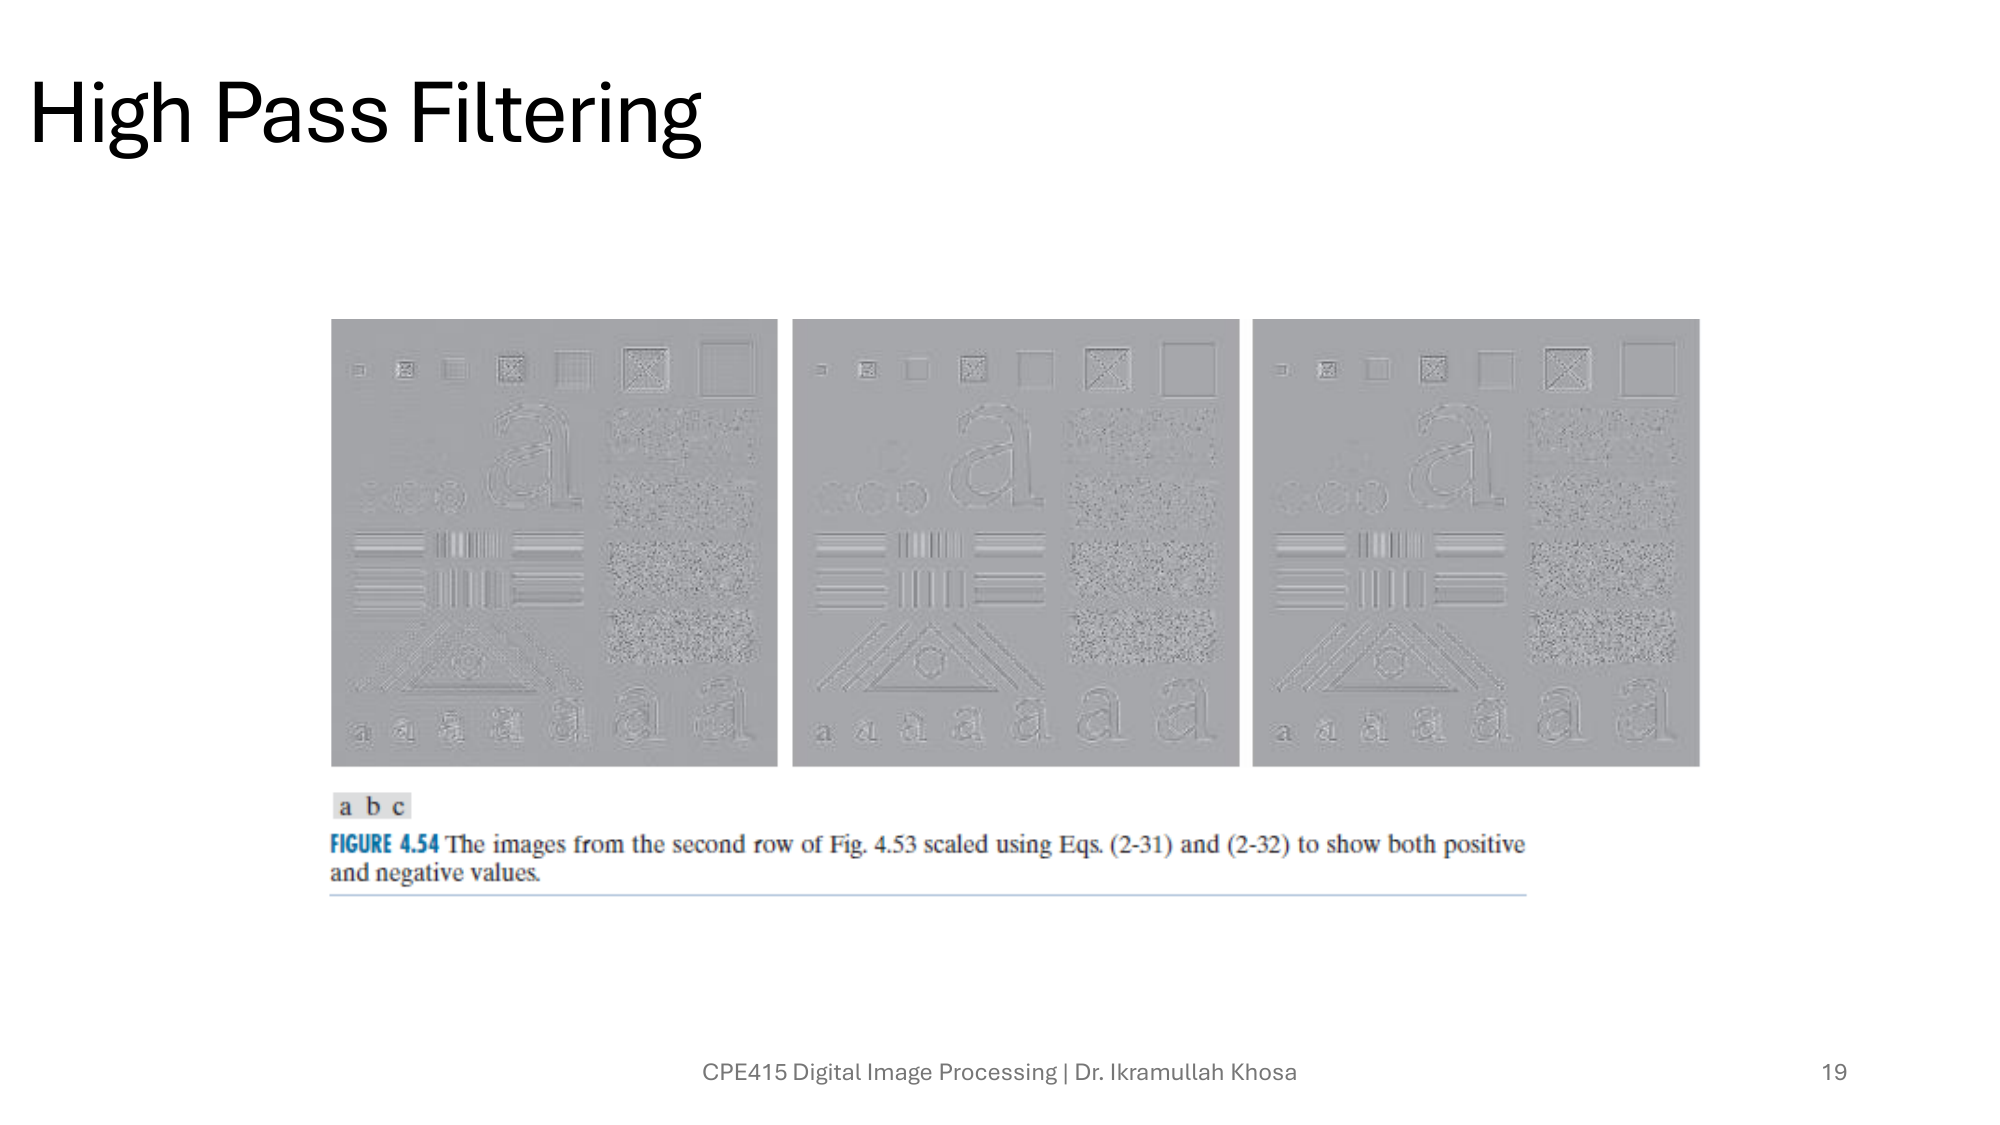
\includegraphics[width=0.95\textwidth]{images/slide10-19.png}
    \caption{Notch filtering example: Removing periodic interference from Saturn ring image (Figure 4.65)}
    \label{fig:saturn_notch}
\end{figure}

\begin{deepexplanation}
\textbf{DEEP ANALYSIS - Figure \ref{fig:saturn_notch}: Classic Notch Filtering Application}

\textbf{What This Figure Shows:}
A famous example from the textbook (Figure 4.65) demonstrating notch filtering on a satellite image of Saturn's rings that contains periodic interference patterns.

\textbf{Four-Panel Breakdown:}
\begin{enumerate}
    \item \textbf{Original image}: Saturn rings corrupted by periodic interference (visible as regular stripes or patterns overlaid on the rings)
    
    \item \textbf{Spectrum}: The Fourier transform magnitude shows the DC peak at center plus symmetric bright spots corresponding to the interference frequency
    
    \item \textbf{Notch filter}: A filter designed with ``holes'' (zeros) at the interference spike locations, shown as dark spots on a white background
    
    \item \textbf{Result}: Cleaned image with interference removed, revealing the underlying Saturn ring structure
\end{enumerate}

\textbf{Why This Works:}
\begin{itemize}
    \item Periodic interference appears as discrete frequency spikes
    \item These spikes are separate from the image content frequencies
    \item Surgically removing only those spikes eliminates the pattern
    \item Minimal collateral damage to desired image content
\end{itemize}

\textbf{Notch Filter Construction:}
For noise spikes at $(u_k, v_k)$:
\[
H_{notch}(u, v) = \prod_{k=1}^{K} H_k(u, v)
\]
where each $H_k$ is a highpass filter centered at $(u_k, v_k)$ and its conjugate.

\textbf{Conjugate Symmetry Requirement:}
For real images, $F(-u, -v) = F^*(u, v)$, so notch filters must come in pairs: if you notch at $(u_k, v_k)$, you must also notch at $(-u_k, -v_k)$.

\textbf{Practical Workflow:}
\begin{enumerate}
    \item Compute and display log-magnitude spectrum
    \item Identify bright spots away from center (interference spikes)
    \item Record their $(u, v)$ coordinates
    \item Design Butterworth notch at each location
    \item Apply filter and inverse transform
\end{enumerate}
\end{deepexplanation}

%==============================================================================
\section{Highpass Filtering}
%==============================================================================

Highpass filters are the complement of lowpass filters, designed to emphasize edges and fine details while attenuating smooth regions.

\subsection{Highpass Filter Types}

\begin{mathbox}
\textbf{Highpass from Lowpass Relationship:}
\[
H_{HP}(u, v) = 1 - H_{LP}(u, v)
\]
This relationship holds for all three filter types.
\end{mathbox}

\begin{figure}[H]
    \centering
    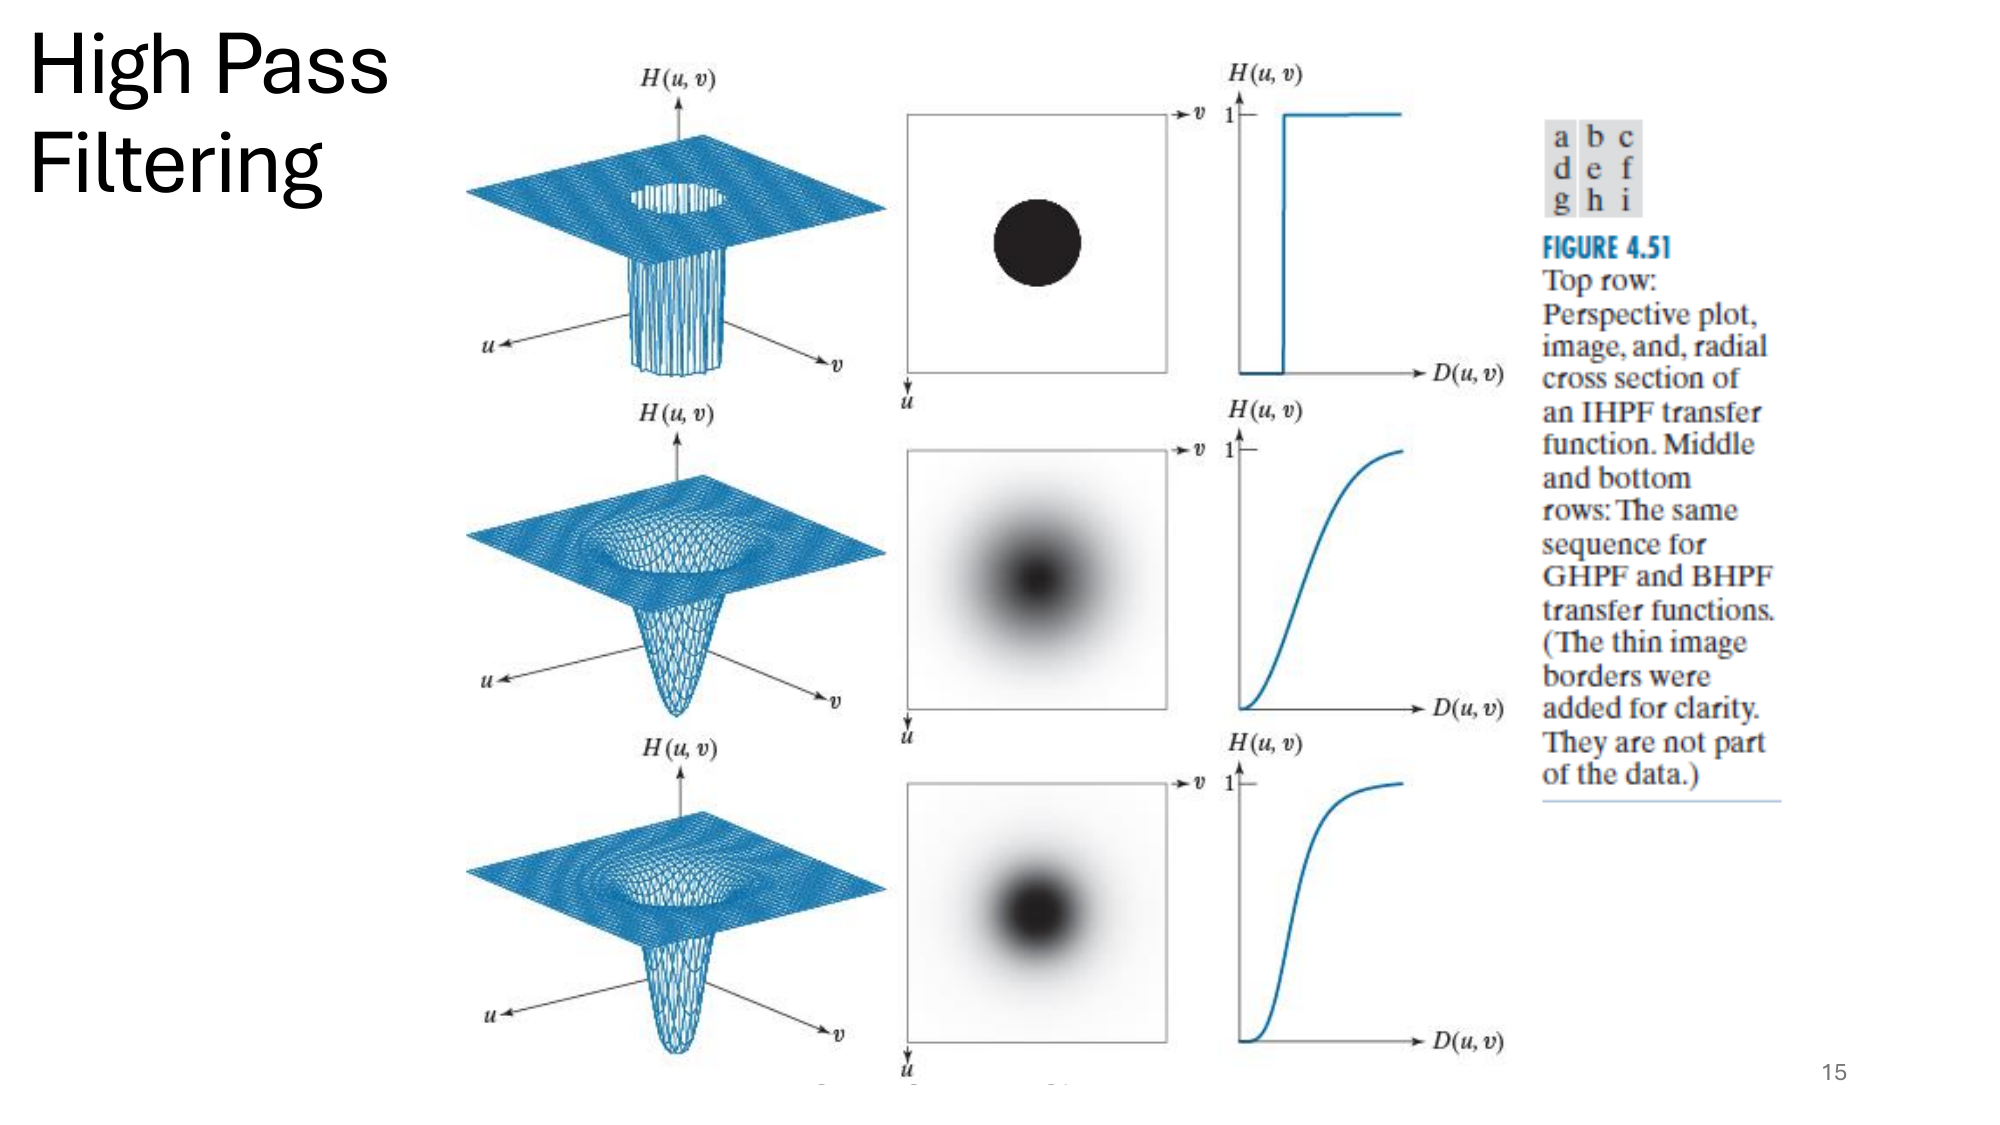
\includegraphics[width=0.9\textwidth]{images/slide10-15.png}
    \caption{Highpass filters: 3D perspective plots and radial cross-sections for Ideal, Gaussian, and Butterworth types}
    \label{fig:hpf_types}
\end{figure}

\begin{deepexplanation}
\textbf{DEEP ANALYSIS - Figure \ref{fig:hpf_types}: Comparing Highpass Filter Shapes}

\textbf{What This Figure Shows:}
A side-by-side comparison of the three main highpass filter types, showing both their 3D frequency response surfaces and 1D radial cross-sections.

\textbf{Ideal Highpass Filter (IHPF):}
\[
H(u, v) = \begin{cases} 0 & D(u, v) \leq D_0 \\ 1 & D(u, v) > D_0 \end{cases}
\]
\begin{itemize}
    \item Zero inside cutoff radius, one outside
    \item Sharp transition at $D_0$
    \item Produces severe ringing around edges
\end{itemize}

\textbf{Gaussian Highpass Filter (GHPF):}
\[
H(u, v) = 1 - e^{-D(u, v)^2 / 2D_0^2}
\]
\begin{itemize}
    \item Smoothest possible transition
    \item Zero at origin, asymptotically approaches 1
    \item No ringing, natural appearance
\end{itemize}

\textbf{Butterworth Highpass Filter (BHPF):}
\[
H(u, v) = \frac{1}{1 + [D_0/D(u, v)]^{2n}}
\]
\begin{itemize}
    \item Note: $D_0$ is in numerator (opposite of lowpass)
    \item Adjustable sharpness via order $n$
    \item At $D = D_0$: $H = 0.5$
\end{itemize}

\textbf{Visual Characteristics:}
\begin{itemize}
    \item 3D plots: ``Bowl'' shapes with low center (DC blocked)
    \item Cross-sections: Start at zero, rise to one at high frequencies
    \item IHPF: Step function; GHPF: Gradual S-curve; BHPF: Intermediate
\end{itemize}

\textbf{Practical Implications:}
Highpass filtering removes the average brightness (DC component), so results often need rescaling or offset addition for proper viewing.
\end{deepexplanation}

\subsection{Highpass Filter Transfer Functions Summary}

\begin{figure}[H]
    \centering
    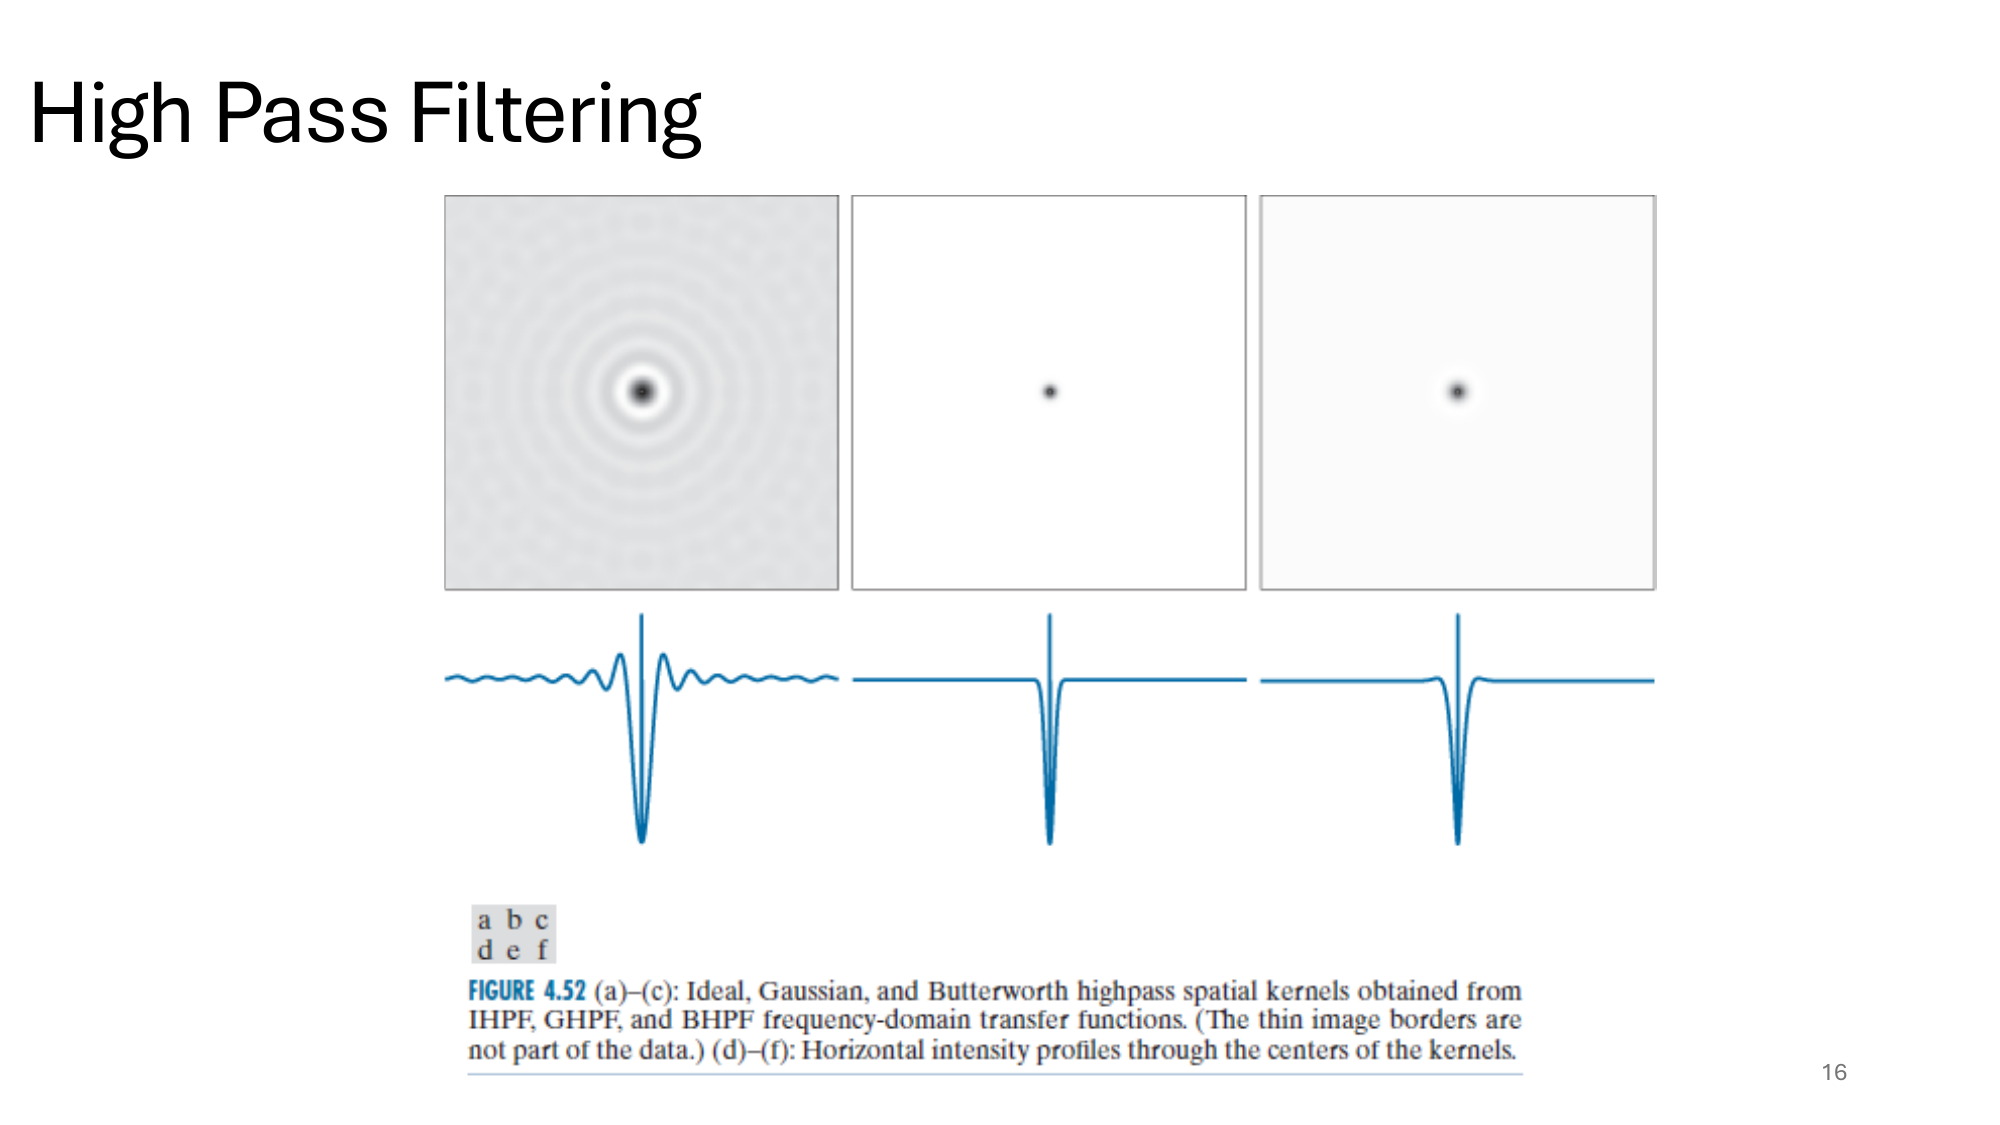
\includegraphics[width=0.9\textwidth]{images/slide10-16.png}
    \caption{Summary table of highpass filter transfer functions: Ideal, Butterworth, and Gaussian}
    \label{fig:hpf_table}
\end{figure}

\begin{deepexplanation}
\textbf{DEEP ANALYSIS - Figure \ref{fig:hpf_table}: Highpass Filter Equations}

\textbf{What This Table Provides:}
A comprehensive reference of the mathematical definitions for the three main highpass filter types.

\textbf{Key Relationships to Lowpass:}
Each highpass filter is simply 1 minus the corresponding lowpass:
\begin{itemize}
    \item IHPF = 1 - ILPF
    \item BHPF = 1 - BLPF
    \item GHPF = 1 - GLPF
\end{itemize}

\textbf{Transfer Functions:}
\begin{center}
\begin{tabular}{|l|c|}
\hline
\textbf{Type} & \textbf{Transfer Function} \\
\hline
Ideal & $H = \begin{cases} 0, & D \leq D_0 \\ 1, & D > D_0 \end{cases}$ \\
\hline
Butterworth & $H = \frac{1}{1 + (D_0/D)^{2n}}$ \\
\hline
Gaussian & $H = 1 - e^{-D^2/2D_0^2}$ \\
\hline
\end{tabular}
\end{center}

\textbf{DC Behavior:}
At $D(u,v) = 0$ (the DC component):
\begin{itemize}
    \item All highpass filters: $H(0,0) = 0$
    \item This means the average image brightness is completely removed
    \item Output has zero mean (balanced around gray)
\end{itemize}

\textbf{High-Frequency Behavior:}
As $D \to \infty$: $H \to 1$ for all types, meaning very high frequencies pass unchanged.
\end{deepexplanation}

%==============================================================================
\section{High-Frequency Emphasis and Image Sharpening}
%==============================================================================

\subsection{High-Frequency Emphasis Filtering}

Pure highpass filtering removes the DC component, making images difficult to view. High-frequency emphasis (HFE) preserves the average brightness while boosting edges.

\begin{mathbox}
\textbf{High-Frequency Emphasis Filter:}
\[
H_{HFE}(u, v) = k_1 + k_2 \cdot H_{HP}(u, v)
\]
where $k_1 \geq 0$ controls DC preservation and $k_2 \geq 0$ controls emphasis strength.
\end{mathbox}

\begin{figure}[H]
    \centering
    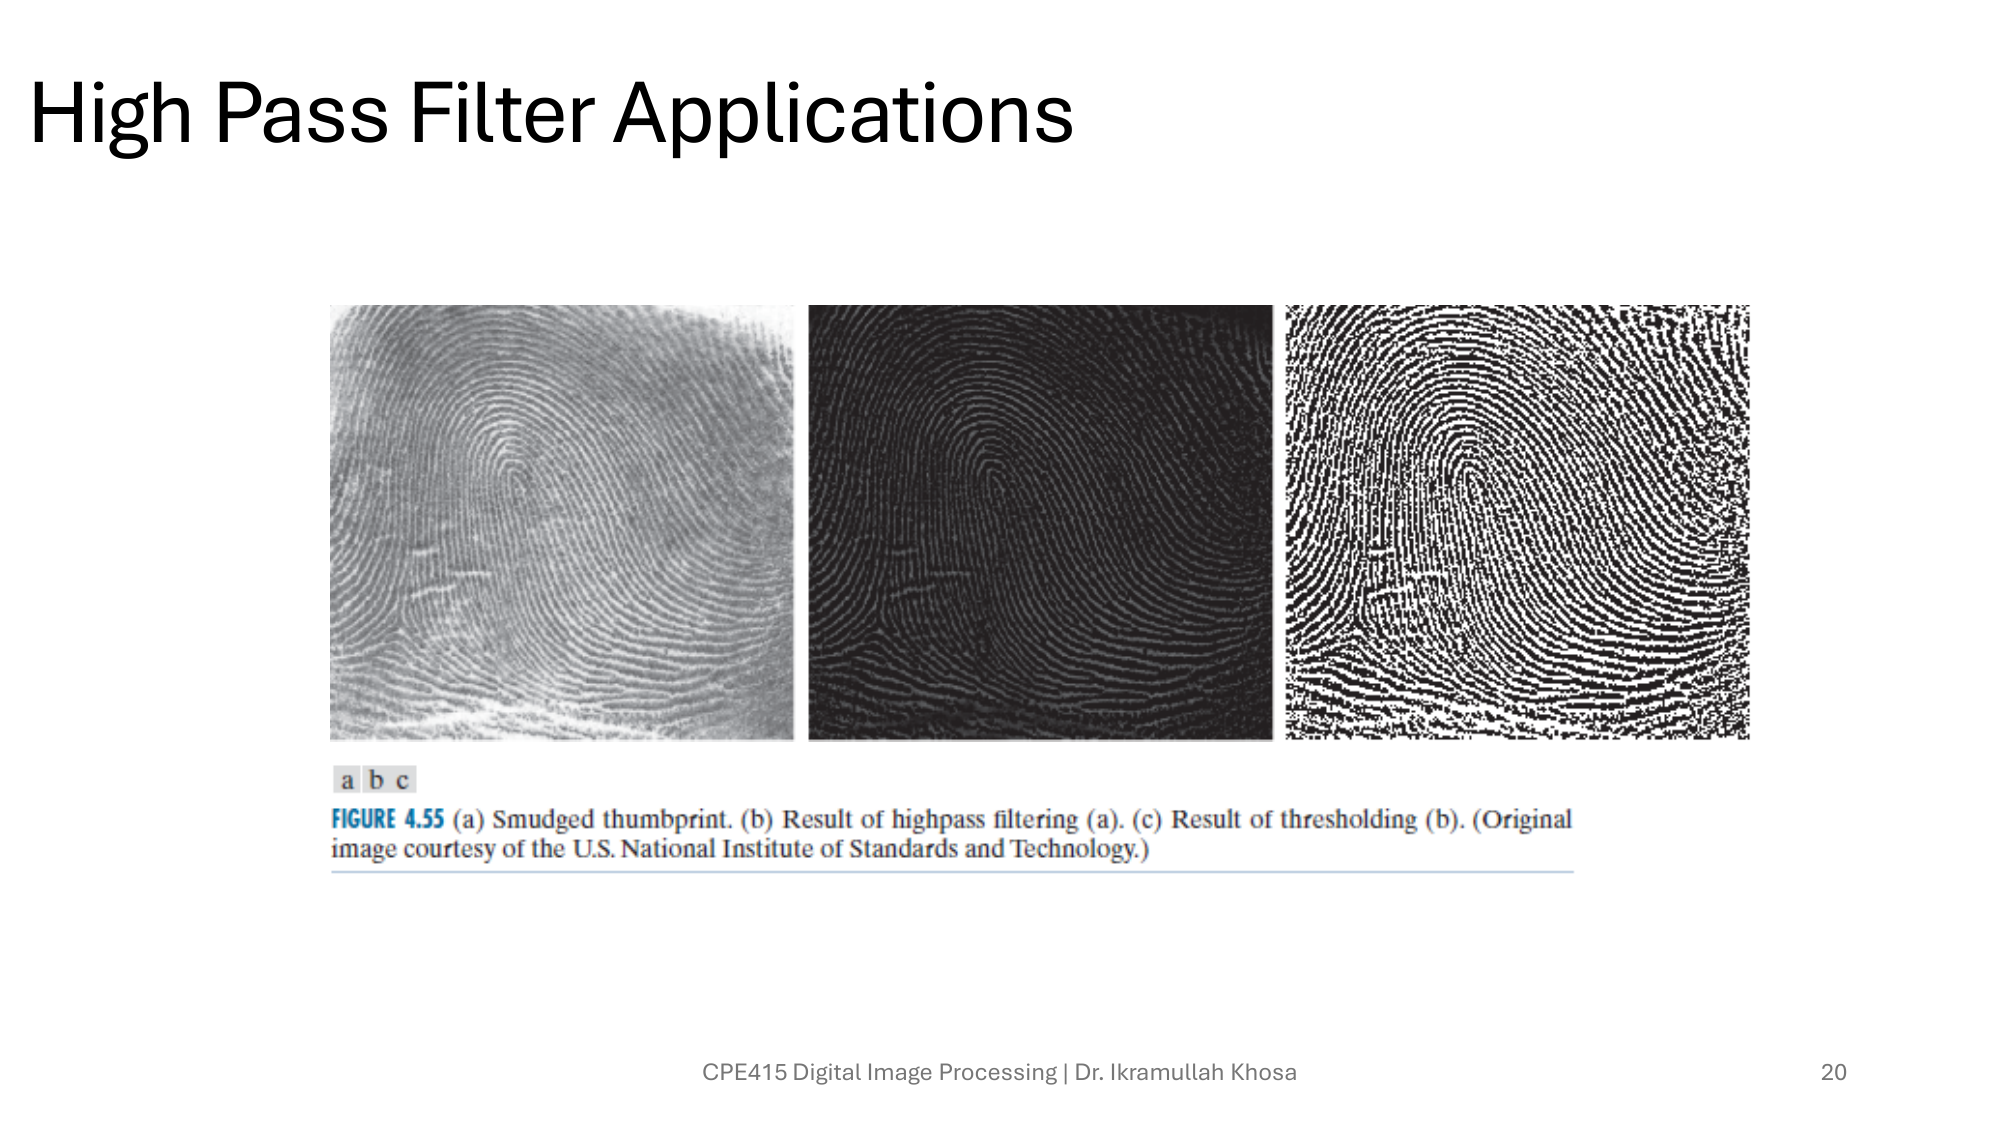
\includegraphics[width=0.95\textwidth]{images/slide10-20.png}
    \caption{High-frequency emphasis filtering comparison: original, pure highpass, and HFE-enhanced results}
    \label{fig:hfe_comparison}
\end{figure}

\begin{deepexplanation}
\textbf{DEEP ANALYSIS - Figure \ref{fig:hfe_comparison}: HFE in Practice}

\textbf{What This Figure Demonstrates:}
A side-by-side comparison showing the difference between pure highpass filtering and high-frequency emphasis, illustrating why HFE is preferred for image sharpening.

\textbf{Panel Comparison:}
\begin{itemize}
    \item \textbf{Original image}: Unprocessed input
    \item \textbf{Pure highpass result}: Edges visible but image appears ``flat'' with no average brightness; DC component removed
    \item \textbf{HFE result}: Sharpened image with natural appearance; edges enhanced while preserving overall brightness
\end{itemize}

\textbf{Mathematical Relationship:}
\[
H_{HFE} = k_1 + k_2(1 - H_{LP}) = (k_1 + k_2) - k_2 \cdot H_{LP}
\]

\textbf{Common Parameter Choices:}
\begin{itemize}
    \item $k_1 = 1, k_2 = 1$: Preserves DC, doubles high frequencies
    \item $k_1 = 0.5, k_2 = 1$: Mild DC reduction with edge boost
    \item $k_1 = 0, k_2 = 1$: Pure highpass (no DC)
\end{itemize}

\textbf{Frequency Response Interpretation:}
\begin{itemize}
    \item At DC ($D = 0$): $H_{HFE} = k_1$ (DC scaled, not removed)
    \item At high frequencies: $H_{HFE} \approx k_1 + k_2$ (amplified)
    \item Net effect: High frequencies boosted relative to low frequencies
\end{itemize}

\textbf{Equivalence to Unsharp Masking:}
In the spatial domain, this is equivalent to:
\[
g = f + k_2(f - f_{blur}) = \text{original} + k_2 \times \text{edges}
\]
HFE is the frequency-domain implementation of unsharp masking.
\end{deepexplanation}

%==============================================================================
\section{Homomorphic Filtering}
%==============================================================================

Homomorphic filtering is a powerful technique for simultaneously correcting non-uniform illumination and enhancing contrast in images.

\subsection{The Illumination-Reflectance Model}

\begin{mathbox}
\textbf{Image Formation Model:}
An image $f(x, y)$ can be modeled as the product of illumination and reflectance:
\[
f(x, y) = i(x, y) \cdot r(x, y)
\]
where:
\begin{itemize}
    \item $i(x, y)$ = illumination component (lighting conditions)
    \item $r(x, y)$ = reflectance component (object properties)
\end{itemize}
\end{mathbox}

\begin{figure}[H]
    \centering
    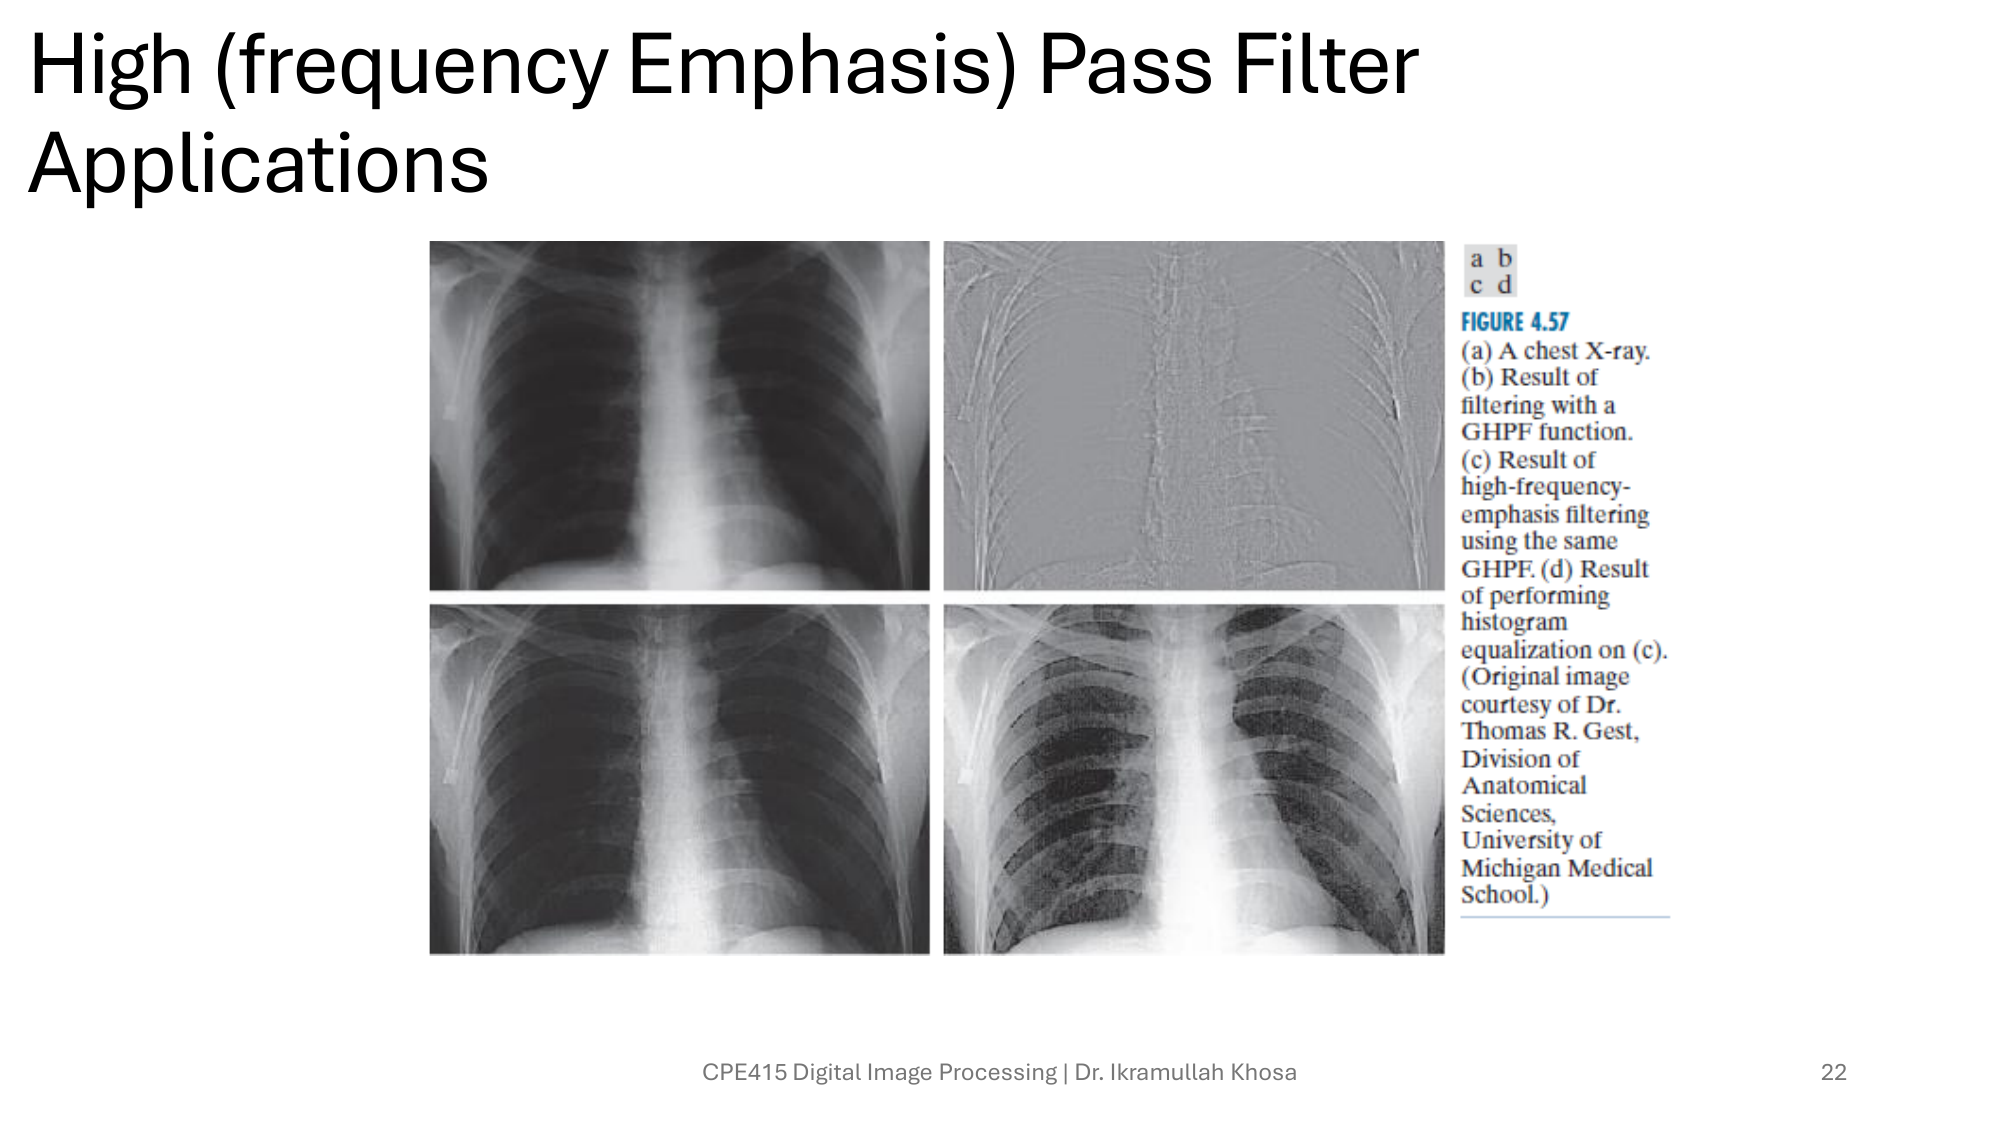
\includegraphics[width=0.9\textwidth]{images/slide10-22.png}
    \caption{Homomorphic filtering system block diagram}
    \label{fig:homomorphic_system}
\end{figure}

\begin{deepexplanation}
\textbf{DEEP ANALYSIS - Figure \ref{fig:homomorphic_system}: The Homomorphic Filtering Pipeline}

\textbf{What This Figure Shows:}
The complete processing chain for homomorphic filtering, illustrating how the multiplicative image model is converted to an additive one for linear filtering.

\textbf{Processing Steps:}
\begin{enumerate}
    \item \textbf{Logarithm}: Convert $f = i \cdot r$ to $\ln(f) = \ln(i) + \ln(r)$
    \item \textbf{Fourier Transform}: Transform to frequency domain
    \item \textbf{Filter}: Apply homomorphic filter $H(u,v)$
    \item \textbf{Inverse Fourier Transform}: Return to spatial domain
    \item \textbf{Exponential}: Convert back: $e^{g} = i' \cdot r'$
\end{enumerate}

\textbf{Why Take the Logarithm?}
The Fourier transform is a linear operation. To apply it to a multiplicative model:
\[
\ln(f) = \ln(i \cdot r) = \ln(i) + \ln(r)
\]
Now we have a sum, and filtering affects each component separately.

\textbf{Key Insight:}
\begin{itemize}
    \item Illumination $i(x,y)$: Varies slowly → Low frequencies
    \item Reflectance $r(x,y)$: Contains edges/details → High frequencies
\end{itemize}
This separation allows us to compress illumination variations while enhancing reflectance details.
\end{deepexplanation}

\subsection{The Homomorphic Filter Function}

\begin{figure}[H]
    \centering
    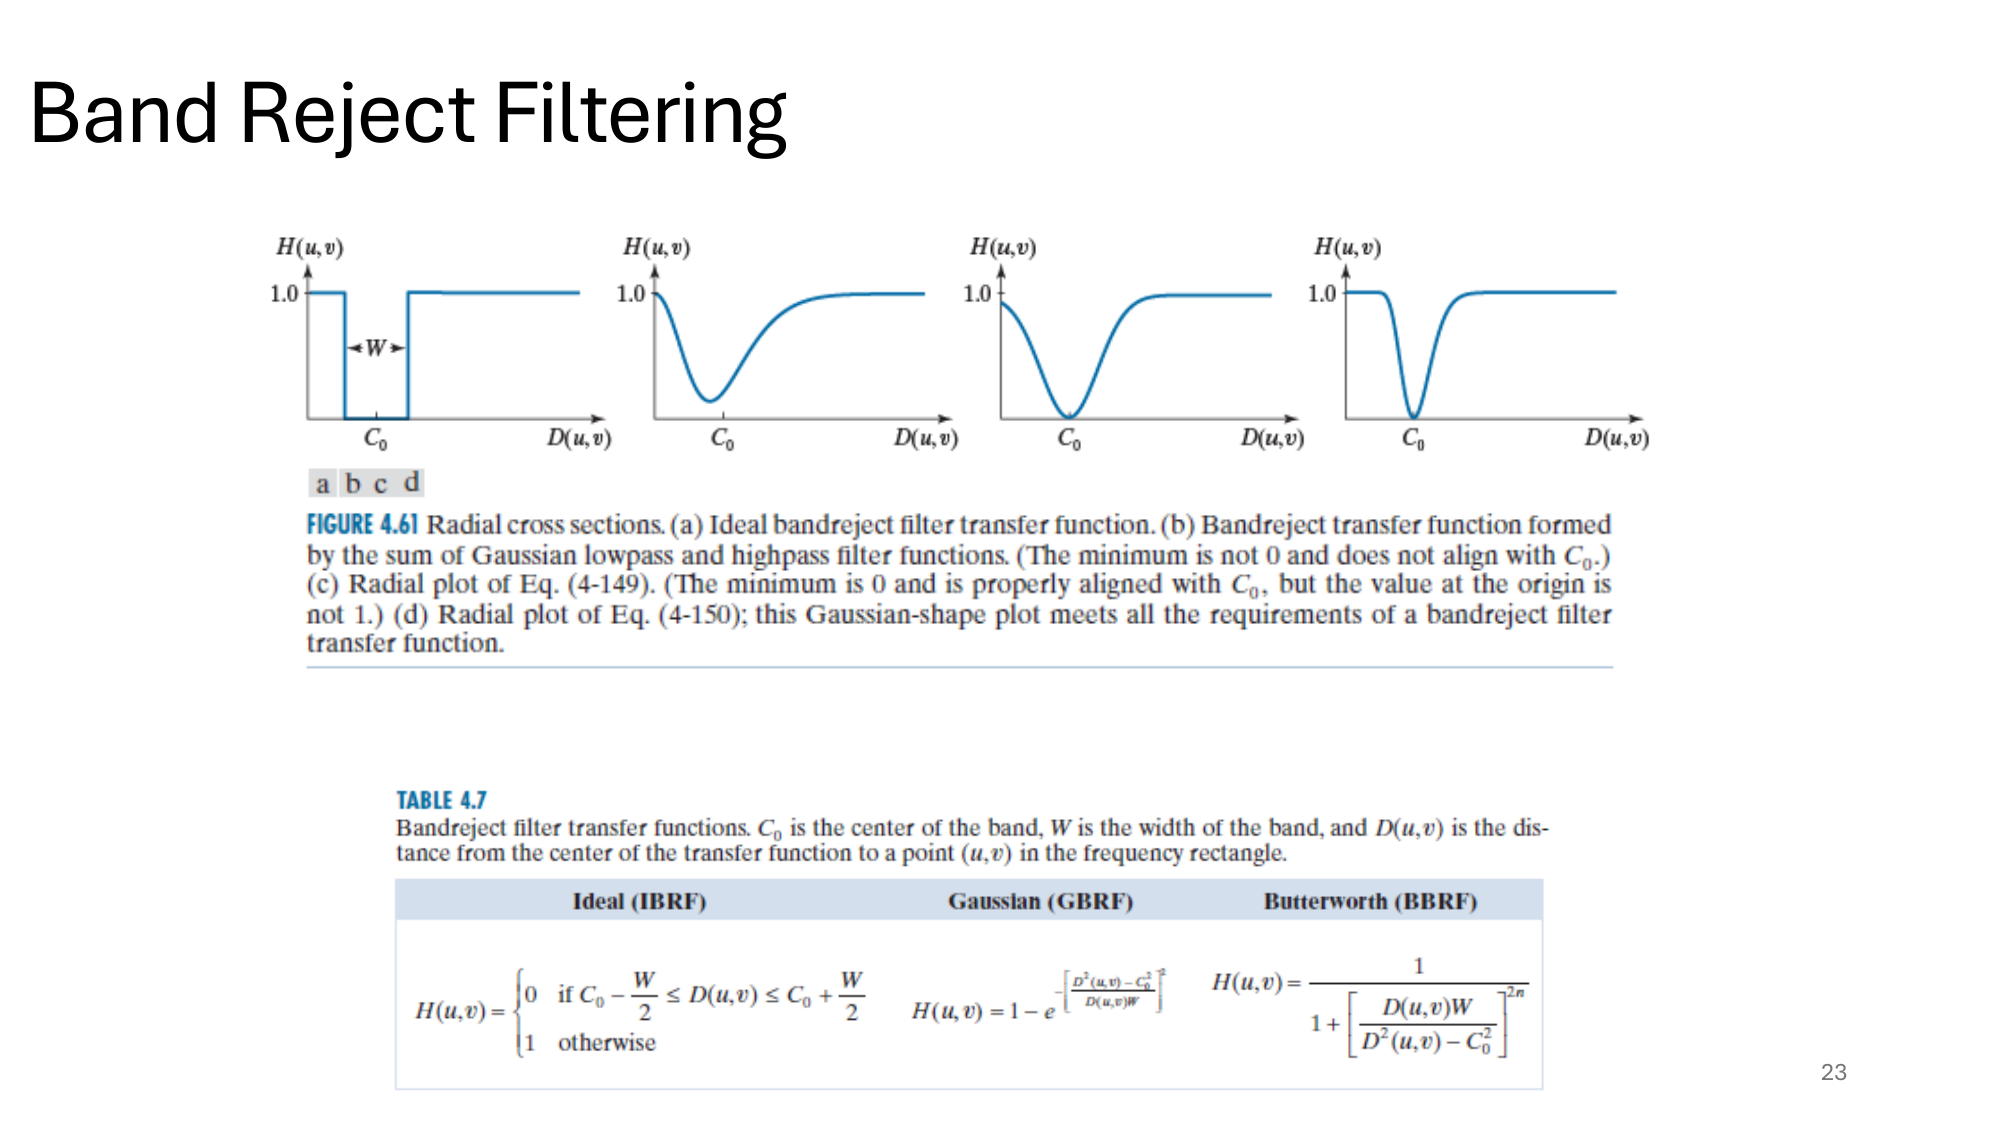
\includegraphics[width=0.85\textwidth]{images/slide10-23.png}
    \caption{Homomorphic filter transfer function $H(u,v)$}
    \label{fig:homomorphic_filter}
\end{figure}

\begin{deepexplanation}
\textbf{DEEP ANALYSIS - Figure \ref{fig:homomorphic_filter}: Designing the Filter}

\textbf{What This Figure Shows:}
The frequency response of a typical homomorphic filter, characterized by different gain values at low and high frequencies.

\textbf{Filter Equation:}
\[
H(u, v) = (\gamma_H - \gamma_L)\left[1 - e^{-c[D(u,v)^2/D_0^2]}\right] + \gamma_L
\]

\textbf{Key Parameters:}
\begin{itemize}
    \item $\gamma_L < 1$: Gain at low frequencies (attenuates illumination)
    \item $\gamma_H > 1$: Gain at high frequencies (amplifies reflectance/details)
    \item $D_0$: Cutoff frequency (transition point)
    \item $c$: Controls transition sharpness
\end{itemize}

\textbf{Filter Behavior:}
\begin{itemize}
    \item At $D = 0$: $H(0,0) = \gamma_L$ (illumination compressed)
    \item At $D \to \infty$: $H \to \gamma_H$ (details boosted)
    \item Smooth transition between extremes
\end{itemize}

\textbf{Typical Values:}
\begin{itemize}
    \item $\gamma_L = 0.25$ to $0.5$ (reduce illumination by 2-4×)
    \item $\gamma_H = 1.5$ to $2.0$ (boost details by 1.5-2×)
\end{itemize}
\end{deepexplanation}

\begin{figure}[H]
    \centering
    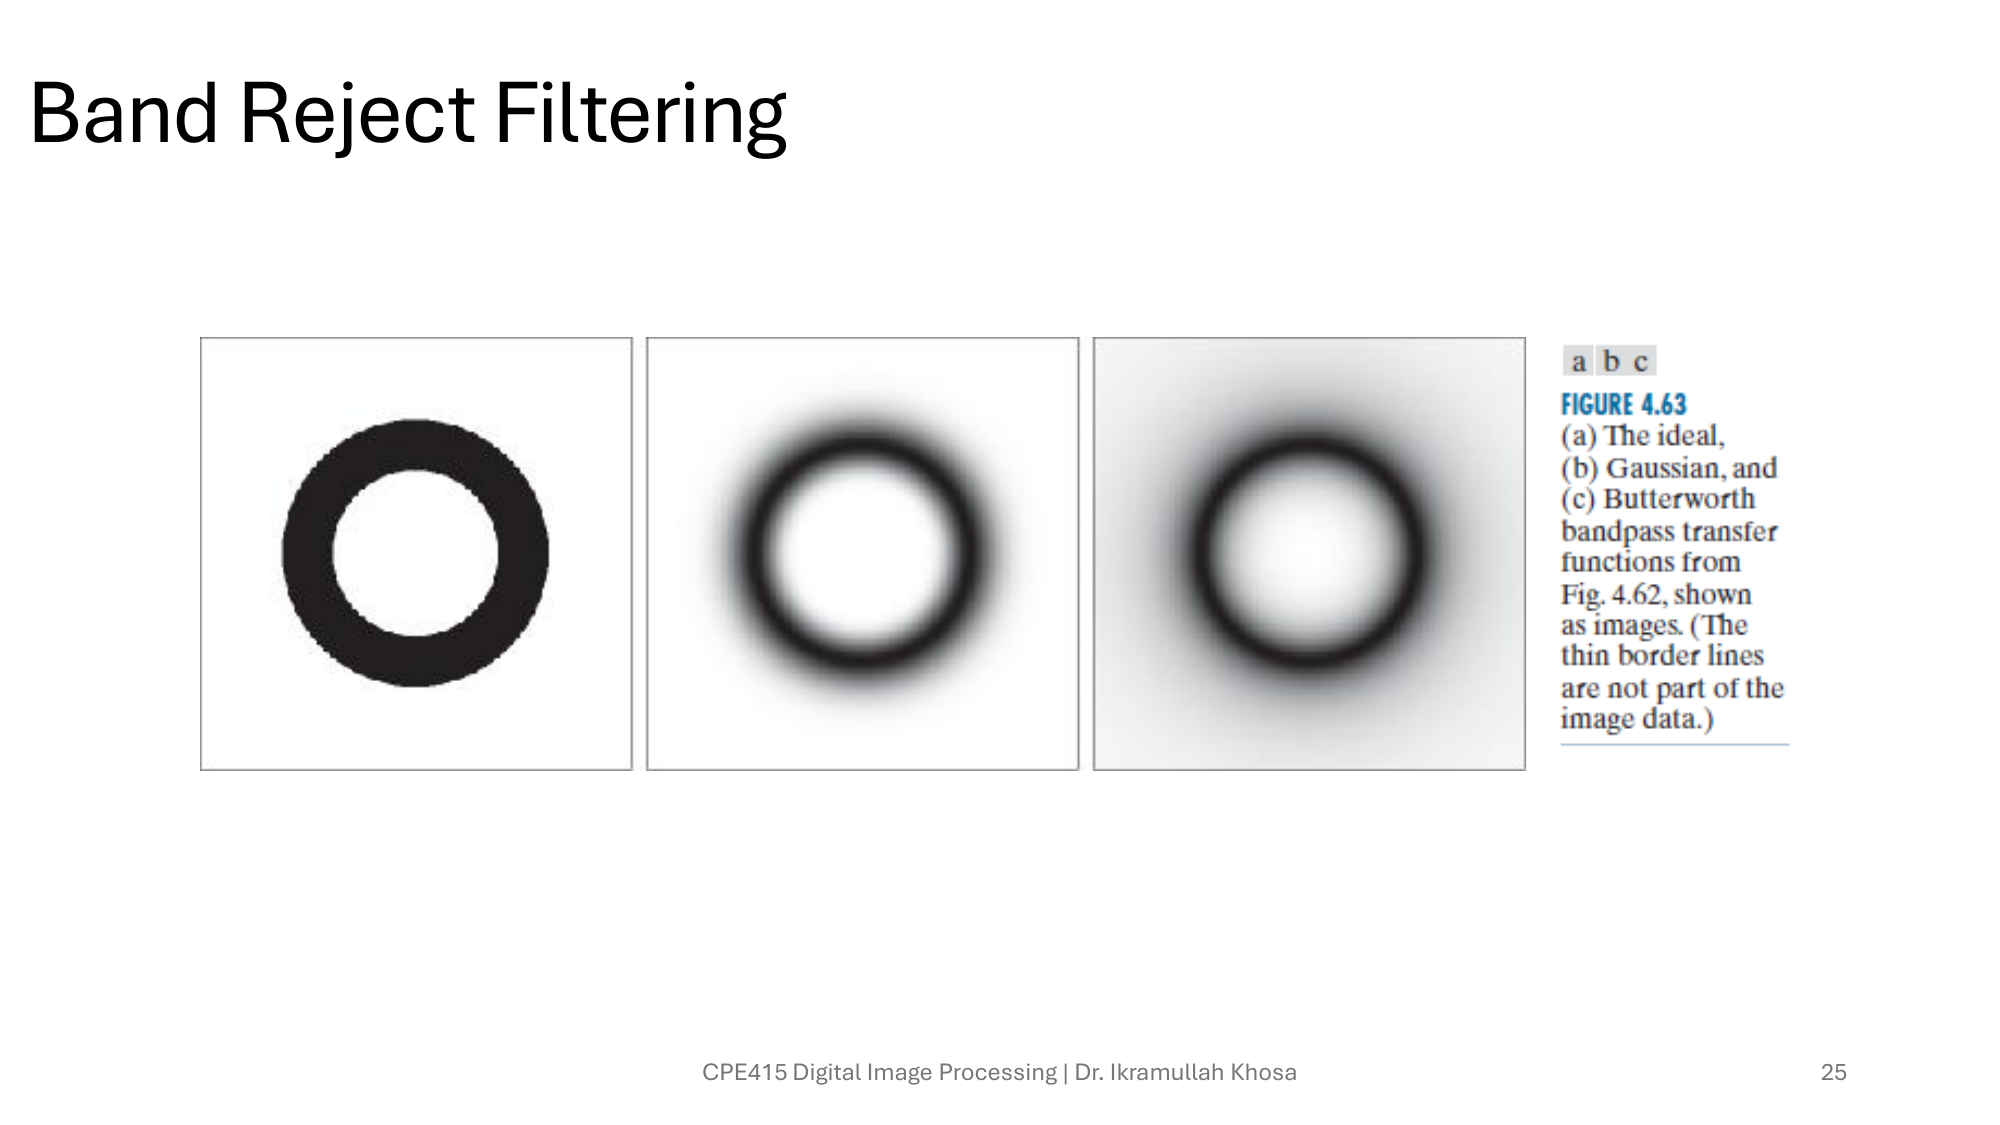
\includegraphics[width=0.8\textwidth]{images/slide10-25.png}
    \caption{Homomorphic filter cross-section showing $\gamma_L$ and $\gamma_H$ parameters}
    \label{fig:homomorphic_crosssection}
\end{figure}

\begin{deepexplanation}
\textbf{DEEP ANALYSIS - Figure \ref{fig:homomorphic_crosssection}: Understanding the Filter Profile}

\textbf{What This Figure Shows:}
A one-dimensional cross-section through the homomorphic filter, clearly showing how the filter transitions from $\gamma_L$ at low frequencies to $\gamma_H$ at high frequencies.

\textbf{Visual Interpretation:}
\begin{itemize}
    \item \textbf{Left side} (low frequencies): Filter value = $\gamma_L$ (typically < 1)
    \item \textbf{Right side} (high frequencies): Filter value = $\gamma_H$ (typically > 1)
    \item \textbf{Transition}: Smooth S-shaped curve centered at $D_0$
\end{itemize}

\textbf{Effect on Image Components:}
\begin{itemize}
    \item Illumination (low freq): Multiplied by $\gamma_L < 1$ → compressed
    \item Reflectance (high freq): Multiplied by $\gamma_H > 1$ → enhanced
\end{itemize}

\textbf{Dynamic Range Compression:}
By compressing illumination variations, the filter reduces the dynamic range of the image while maintaining (even enhancing) local contrast from reflectance. This is particularly useful for:
\begin{itemize}
    \item Images with bright and dark regions
    \item Backlit scenes
    \item Non-uniform lighting conditions
\end{itemize}
\end{deepexplanation}

\subsection{Homomorphic Filtering Results}

\begin{figure}[H]
    \centering
    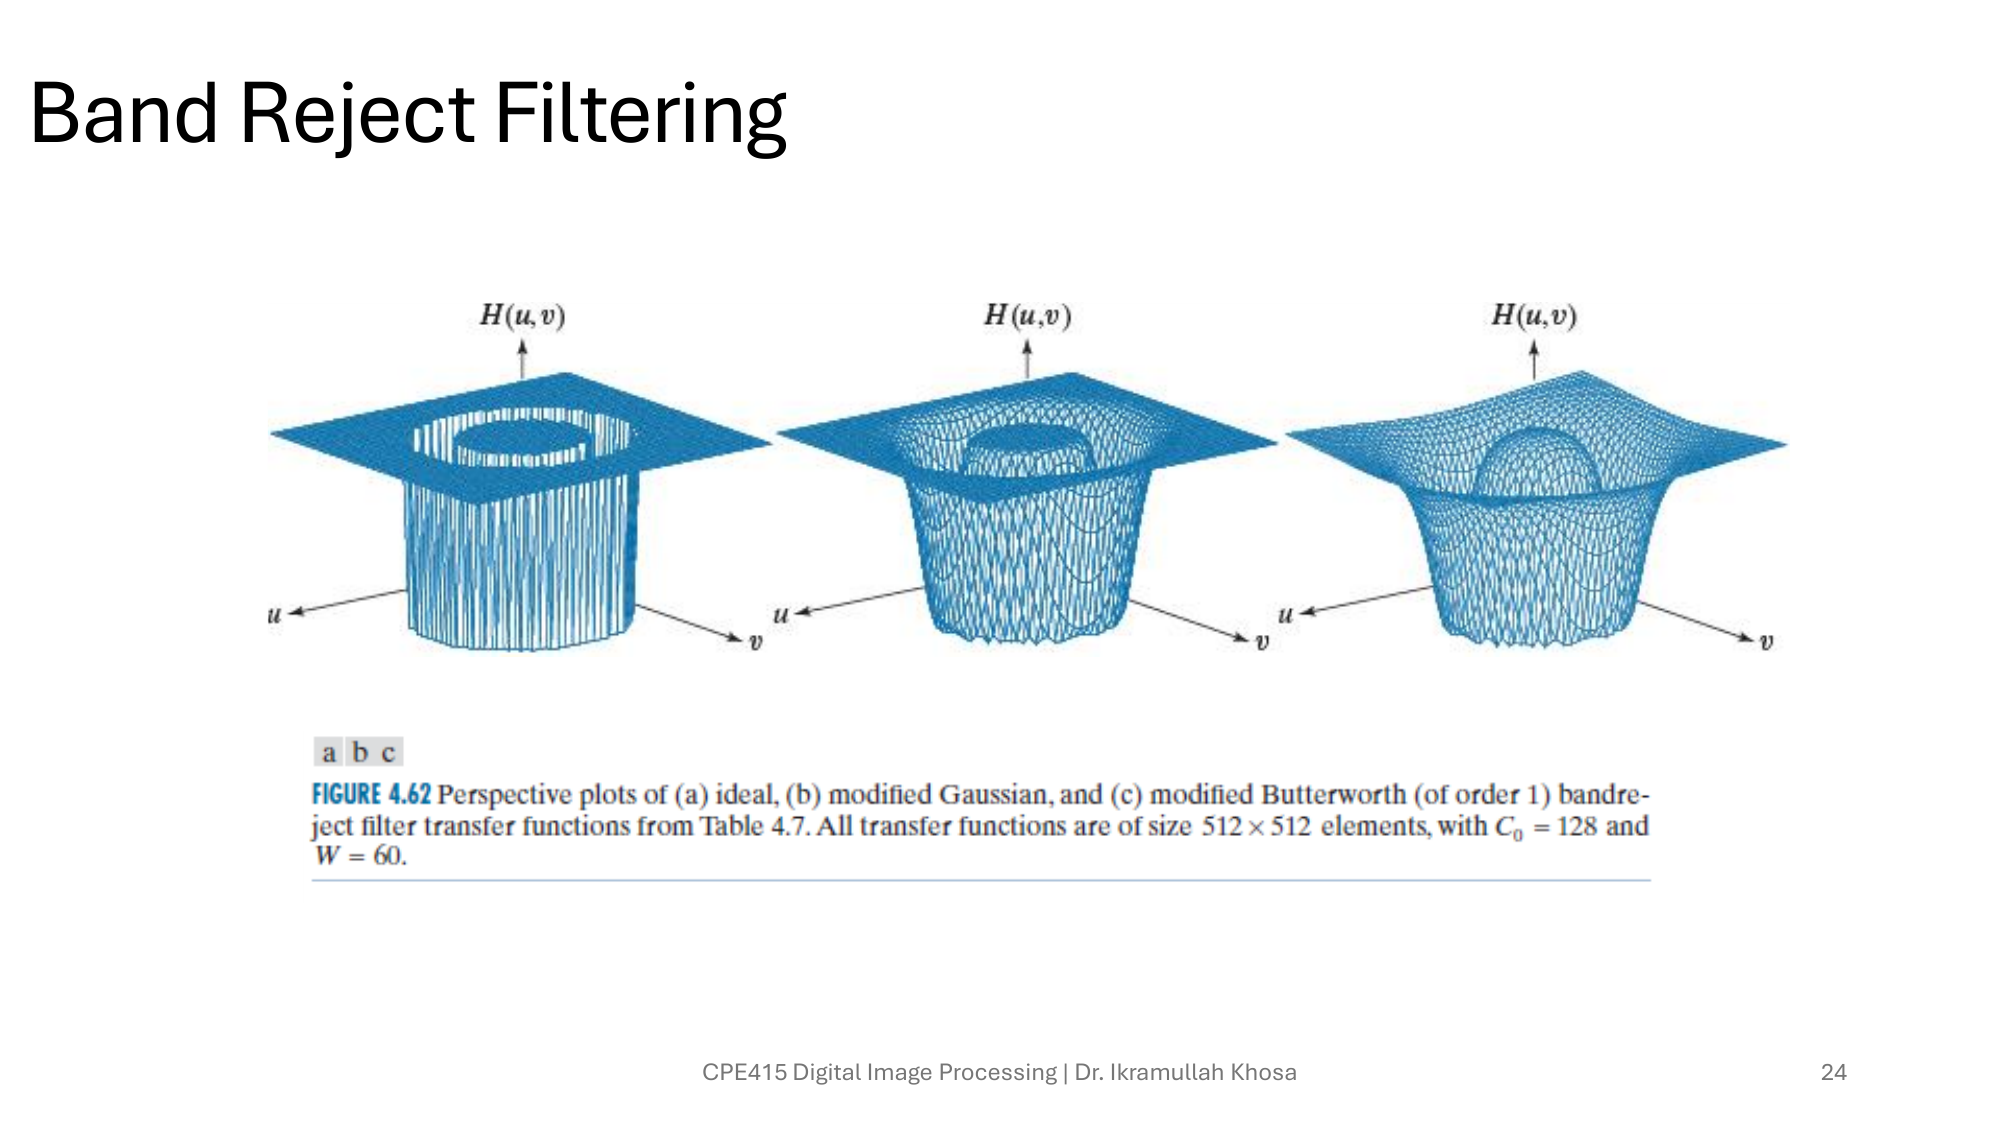
\includegraphics[width=0.95\textwidth]{images/slide10-24.png}
    \caption{Homomorphic filtering example: face image with non-uniform illumination}
    \label{fig:homomorphic_face}
\end{figure}

\begin{deepexplanation}
\textbf{DEEP ANALYSIS - Figure \ref{fig:homomorphic_face}: Practical Application}

\textbf{What This Figure Demonstrates:}
A before-and-after comparison showing homomorphic filtering applied to a face image with non-uniform illumination (one side brighter than the other).

\textbf{Original Image Problems:}
\begin{itemize}
    \item One side of face much brighter than other
    \item Details in dark regions hard to see
    \item Details in bright regions washed out
    \item High dynamic range difficult to display/print
\end{itemize}

\textbf{After Homomorphic Filtering:}
\begin{itemize}
    \item Illumination variations reduced (face appears evenly lit)
    \item Details visible in both previously-dark and previously-bright areas
    \item Overall contrast improved
    \item Dynamic range compressed to displayable levels
\end{itemize}

\textbf{Why It Works:}
The filter simultaneously:
\begin{enumerate}
    \item Compresses the slowly-varying illumination ($\gamma_L < 1$)
    \item Enhances the reflectance edges and details ($\gamma_H > 1$)
\end{enumerate}
This achieves what would be very difficult with simple brightness/contrast adjustments.
\end{deepexplanation}

\begin{figure}[H]
    \centering
    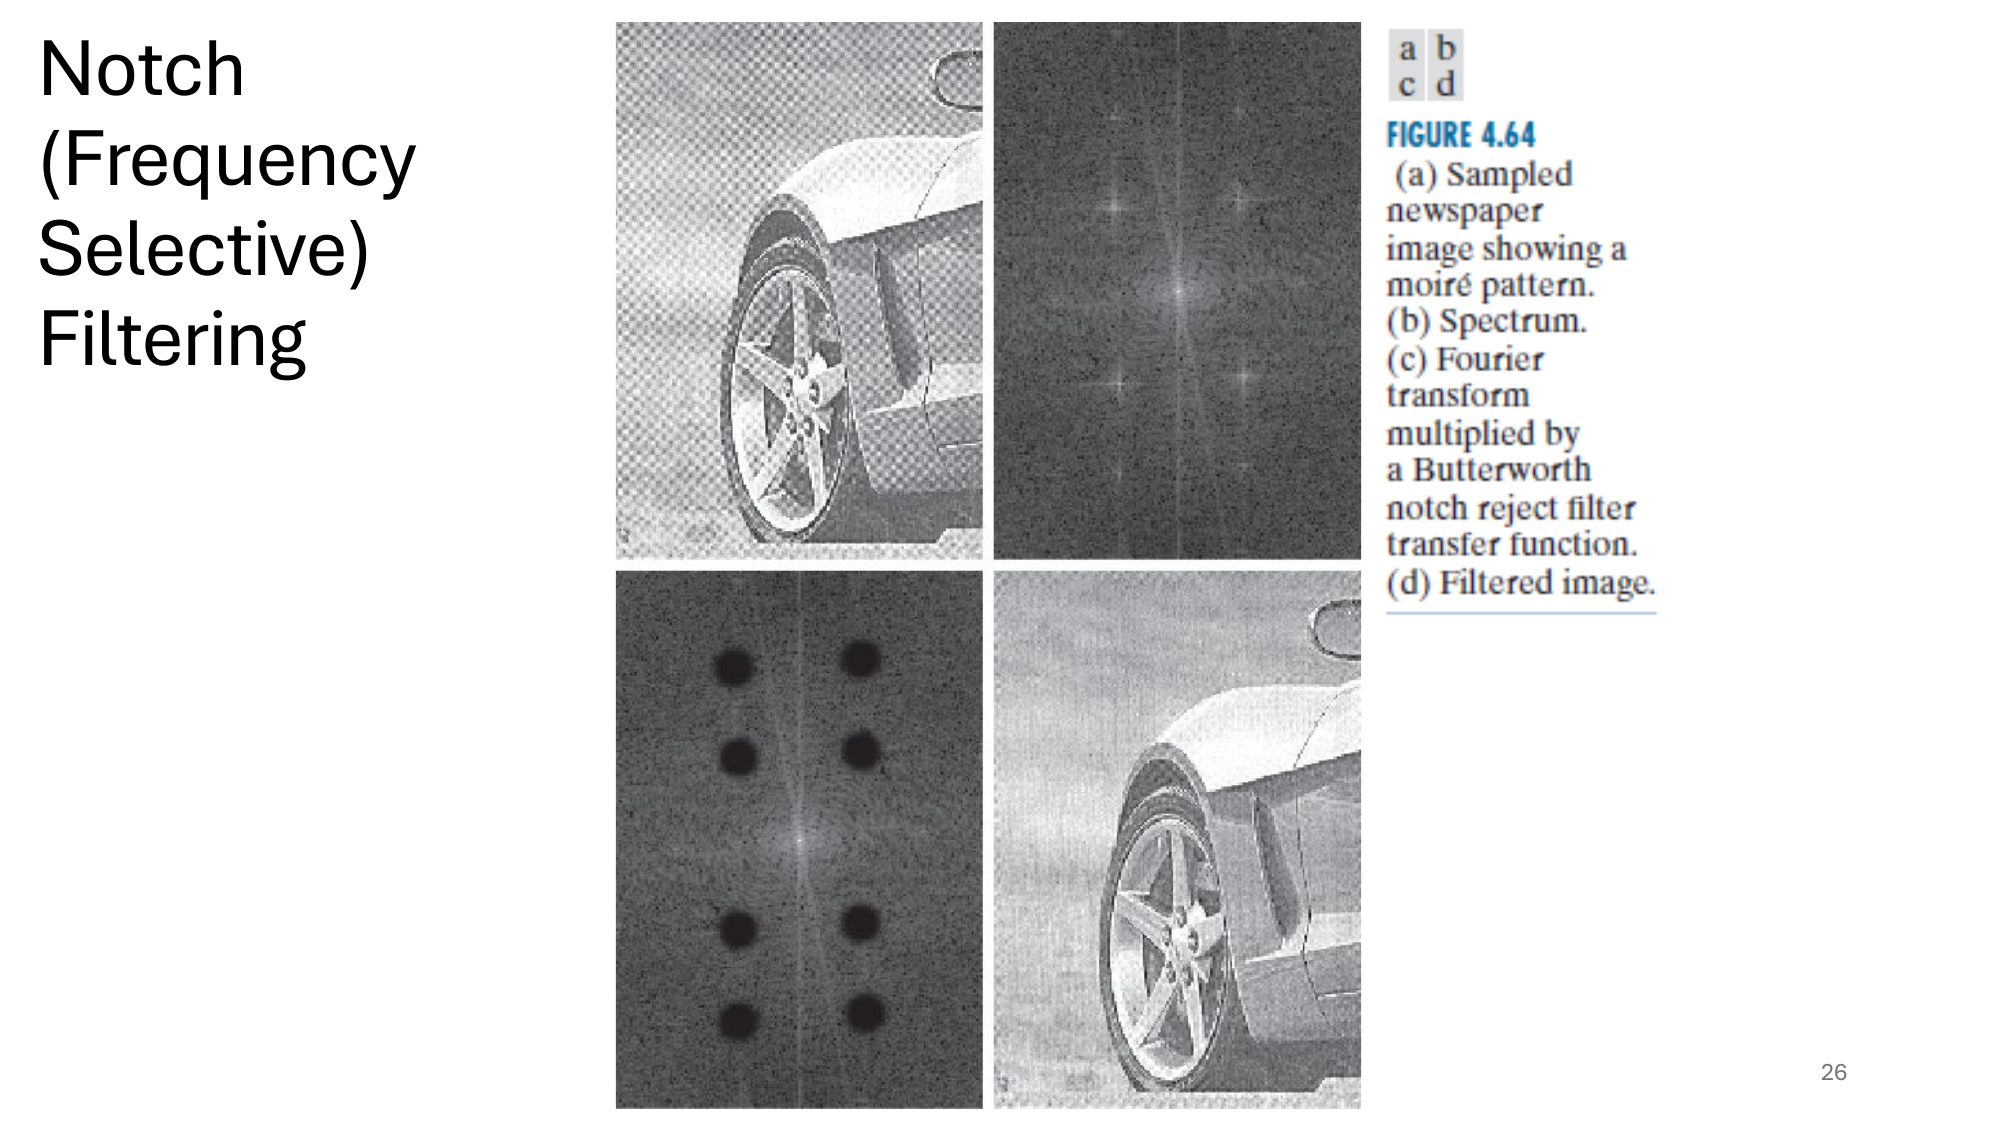
\includegraphics[width=0.95\textwidth]{images/slide10-26.png}
    \caption{Additional homomorphic filtering examples showing illumination correction}
    \label{fig:homomorphic_examples}
\end{figure}

\begin{deepexplanation}
\textbf{DEEP ANALYSIS - Figure \ref{fig:homomorphic_examples}: More Applications}

\textbf{What This Figure Shows:}
Additional examples of homomorphic filtering applied to images with various illumination problems.

\textbf{Common Scenarios Where Homomorphic Filtering Helps:}
\begin{itemize}
    \item Indoor photos with windows (backlit subjects)
    \item Medical images with uneven illumination
    \item Surveillance footage with lighting gradients
    \item Scanned documents with shadows
    \item Satellite/aerial images with varying sun angles
\end{itemize}

\textbf{Parameter Tuning Guidelines:}
\begin{itemize}
    \item More illumination variation → Lower $\gamma_L$
    \item Need more detail enhancement → Higher $\gamma_H$
    \item Coarse illumination gradients → Lower $D_0$
    \item Fine illumination patterns → Higher $D_0$
\end{itemize}

\textbf{Limitations:}
\begin{itemize}
    \item Assumes multiplicative illumination-reflectance model
    \item Cannot handle specular reflections well
    \item May amplify noise in dark regions
    \item Logarithm undefined for zero values (requires offset)
\end{itemize}

\textbf{Preprocessing Step:}
To avoid $\ln(0)$, add small constant: $\ln(f + \epsilon)$ where $\epsilon$ is a small positive value.
\end{deepexplanation}

%==============================================================================
\section{Chapter Summary: Key Takeaways}
%==============================================================================

\begin{importantbox}
\textbf{Essential Concepts to Remember:}

\begin{enumerate}
    \item \textbf{Fourier Transform} decomposes images into sinusoidal basis functions at different frequencies and orientations.
    
    \item \textbf{Sampling Theorem}: Sample rate must exceed twice the maximum frequency (Nyquist rate) to avoid aliasing.
    
    \item \textbf{Aliasing} causes high frequencies to masquerade as low frequencies --- visible as moiré patterns, jagged edges, and false details.
    
    \item \textbf{Convolution Theorem}: Spatial convolution equals frequency multiplication, enabling efficient filtering via FFT.
    
    \item \textbf{Filter Design}:
    \begin{itemize}
        \item Ideal: Sharp cutoff, severe ringing
        \item Butterworth: Adjustable rolloff, controlled ringing
        \item Gaussian: Smooth rolloff, no ringing (optimal for most applications)
    \end{itemize}
    
    \item \textbf{Lowpass} smooths by removing high frequencies; \textbf{Highpass} enhances edges by removing low frequencies.
    
    \item \textbf{Notch filters} surgically remove periodic interference at specific frequency locations.
    
    \item \textbf{FFT} reduces computation from $O(N^2)$ to $O(N \log N)$, making real-time frequency processing possible.
    
    \item \textbf{Phase is crucial}: It carries structural information (edges, positions) more than magnitude does.
\end{enumerate}
\end{importantbox}

\vspace{1cm}

\begin{center}
\textit{``The Fourier transform is perhaps the most important single tool in signal processing, and understanding it thoroughly opens doors to advanced image analysis, compression, and computational photography.''}
\end{center}

\end{document}
